% Options for packages loaded elsewhere
\PassOptionsToPackage{unicode}{hyperref}
\PassOptionsToPackage{hyphens}{url}
\PassOptionsToPackage{dvipsnames,svgnames,x11names}{xcolor}
%
\documentclass[
  letterpaper,
  DIV=11,
  numbers=noendperiod]{scrartcl}

\usepackage{amsmath,amssymb}
\usepackage{iftex}
\ifPDFTeX
  \usepackage[T1]{fontenc}
  \usepackage[utf8]{inputenc}
  \usepackage{textcomp} % provide euro and other symbols
\else % if luatex or xetex
  \usepackage{unicode-math}
  \defaultfontfeatures{Scale=MatchLowercase}
  \defaultfontfeatures[\rmfamily]{Ligatures=TeX,Scale=1}
\fi
\usepackage{lmodern}
\ifPDFTeX\else  
    % xetex/luatex font selection
\fi
% Use upquote if available, for straight quotes in verbatim environments
\IfFileExists{upquote.sty}{\usepackage{upquote}}{}
\IfFileExists{microtype.sty}{% use microtype if available
  \usepackage[]{microtype}
  \UseMicrotypeSet[protrusion]{basicmath} % disable protrusion for tt fonts
}{}
\makeatletter
\@ifundefined{KOMAClassName}{% if non-KOMA class
  \IfFileExists{parskip.sty}{%
    \usepackage{parskip}
  }{% else
    \setlength{\parindent}{0pt}
    \setlength{\parskip}{6pt plus 2pt minus 1pt}}
}{% if KOMA class
  \KOMAoptions{parskip=half}}
\makeatother
\usepackage{xcolor}
\setlength{\emergencystretch}{3em} % prevent overfull lines
\setcounter{secnumdepth}{-\maxdimen} % remove section numbering
% Make \paragraph and \subparagraph free-standing
\ifx\paragraph\undefined\else
  \let\oldparagraph\paragraph
  \renewcommand{\paragraph}[1]{\oldparagraph{#1}\mbox{}}
\fi
\ifx\subparagraph\undefined\else
  \let\oldsubparagraph\subparagraph
  \renewcommand{\subparagraph}[1]{\oldsubparagraph{#1}\mbox{}}
\fi

\usepackage{color}
\usepackage{fancyvrb}
\newcommand{\VerbBar}{|}
\newcommand{\VERB}{\Verb[commandchars=\\\{\}]}
\DefineVerbatimEnvironment{Highlighting}{Verbatim}{commandchars=\\\{\}}
% Add ',fontsize=\small' for more characters per line
\usepackage{framed}
\definecolor{shadecolor}{RGB}{241,243,245}
\newenvironment{Shaded}{\begin{snugshade}}{\end{snugshade}}
\newcommand{\AlertTok}[1]{\textcolor[rgb]{0.68,0.00,0.00}{#1}}
\newcommand{\AnnotationTok}[1]{\textcolor[rgb]{0.37,0.37,0.37}{#1}}
\newcommand{\AttributeTok}[1]{\textcolor[rgb]{0.40,0.45,0.13}{#1}}
\newcommand{\BaseNTok}[1]{\textcolor[rgb]{0.68,0.00,0.00}{#1}}
\newcommand{\BuiltInTok}[1]{\textcolor[rgb]{0.00,0.23,0.31}{#1}}
\newcommand{\CharTok}[1]{\textcolor[rgb]{0.13,0.47,0.30}{#1}}
\newcommand{\CommentTok}[1]{\textcolor[rgb]{0.37,0.37,0.37}{#1}}
\newcommand{\CommentVarTok}[1]{\textcolor[rgb]{0.37,0.37,0.37}{\textit{#1}}}
\newcommand{\ConstantTok}[1]{\textcolor[rgb]{0.56,0.35,0.01}{#1}}
\newcommand{\ControlFlowTok}[1]{\textcolor[rgb]{0.00,0.23,0.31}{#1}}
\newcommand{\DataTypeTok}[1]{\textcolor[rgb]{0.68,0.00,0.00}{#1}}
\newcommand{\DecValTok}[1]{\textcolor[rgb]{0.68,0.00,0.00}{#1}}
\newcommand{\DocumentationTok}[1]{\textcolor[rgb]{0.37,0.37,0.37}{\textit{#1}}}
\newcommand{\ErrorTok}[1]{\textcolor[rgb]{0.68,0.00,0.00}{#1}}
\newcommand{\ExtensionTok}[1]{\textcolor[rgb]{0.00,0.23,0.31}{#1}}
\newcommand{\FloatTok}[1]{\textcolor[rgb]{0.68,0.00,0.00}{#1}}
\newcommand{\FunctionTok}[1]{\textcolor[rgb]{0.28,0.35,0.67}{#1}}
\newcommand{\ImportTok}[1]{\textcolor[rgb]{0.00,0.46,0.62}{#1}}
\newcommand{\InformationTok}[1]{\textcolor[rgb]{0.37,0.37,0.37}{#1}}
\newcommand{\KeywordTok}[1]{\textcolor[rgb]{0.00,0.23,0.31}{#1}}
\newcommand{\NormalTok}[1]{\textcolor[rgb]{0.00,0.23,0.31}{#1}}
\newcommand{\OperatorTok}[1]{\textcolor[rgb]{0.37,0.37,0.37}{#1}}
\newcommand{\OtherTok}[1]{\textcolor[rgb]{0.00,0.23,0.31}{#1}}
\newcommand{\PreprocessorTok}[1]{\textcolor[rgb]{0.68,0.00,0.00}{#1}}
\newcommand{\RegionMarkerTok}[1]{\textcolor[rgb]{0.00,0.23,0.31}{#1}}
\newcommand{\SpecialCharTok}[1]{\textcolor[rgb]{0.37,0.37,0.37}{#1}}
\newcommand{\SpecialStringTok}[1]{\textcolor[rgb]{0.13,0.47,0.30}{#1}}
\newcommand{\StringTok}[1]{\textcolor[rgb]{0.13,0.47,0.30}{#1}}
\newcommand{\VariableTok}[1]{\textcolor[rgb]{0.07,0.07,0.07}{#1}}
\newcommand{\VerbatimStringTok}[1]{\textcolor[rgb]{0.13,0.47,0.30}{#1}}
\newcommand{\WarningTok}[1]{\textcolor[rgb]{0.37,0.37,0.37}{\textit{#1}}}

\providecommand{\tightlist}{%
  \setlength{\itemsep}{0pt}\setlength{\parskip}{0pt}}\usepackage{longtable,booktabs,array}
\usepackage{calc} % for calculating minipage widths
% Correct order of tables after \paragraph or \subparagraph
\usepackage{etoolbox}
\makeatletter
\patchcmd\longtable{\par}{\if@noskipsec\mbox{}\fi\par}{}{}
\makeatother
% Allow footnotes in longtable head/foot
\IfFileExists{footnotehyper.sty}{\usepackage{footnotehyper}}{\usepackage{footnote}}
\makesavenoteenv{longtable}
\usepackage{graphicx}
\makeatletter
\def\maxwidth{\ifdim\Gin@nat@width>\linewidth\linewidth\else\Gin@nat@width\fi}
\def\maxheight{\ifdim\Gin@nat@height>\textheight\textheight\else\Gin@nat@height\fi}
\makeatother
% Scale images if necessary, so that they will not overflow the page
% margins by default, and it is still possible to overwrite the defaults
% using explicit options in \includegraphics[width, height, ...]{}
\setkeys{Gin}{width=\maxwidth,height=\maxheight,keepaspectratio}
% Set default figure placement to htbp
\makeatletter
\def\fps@figure{htbp}
\makeatother

\usepackage{booktabs}
\usepackage{longtable}
\usepackage{array}
\usepackage{multirow}
\usepackage{wrapfig}
\usepackage{float}
\usepackage{colortbl}
\usepackage{pdflscape}
\usepackage{tabu}
\usepackage{threeparttable}
\usepackage{threeparttablex}
\usepackage[normalem]{ulem}
\usepackage{makecell}
\usepackage{xcolor}
\KOMAoption{captions}{tableheading}
\makeatletter
\@ifpackageloaded{caption}{}{\usepackage{caption}}
\AtBeginDocument{%
\ifdefined\contentsname
  \renewcommand*\contentsname{Table of contents}
\else
  \newcommand\contentsname{Table of contents}
\fi
\ifdefined\listfigurename
  \renewcommand*\listfigurename{List of Figures}
\else
  \newcommand\listfigurename{List of Figures}
\fi
\ifdefined\listtablename
  \renewcommand*\listtablename{List of Tables}
\else
  \newcommand\listtablename{List of Tables}
\fi
\ifdefined\figurename
  \renewcommand*\figurename{Figure}
\else
  \newcommand\figurename{Figure}
\fi
\ifdefined\tablename
  \renewcommand*\tablename{Table}
\else
  \newcommand\tablename{Table}
\fi
}
\@ifpackageloaded{float}{}{\usepackage{float}}
\floatstyle{ruled}
\@ifundefined{c@chapter}{\newfloat{codelisting}{h}{lop}}{\newfloat{codelisting}{h}{lop}[chapter]}
\floatname{codelisting}{Listing}
\newcommand*\listoflistings{\listof{codelisting}{List of Listings}}
\makeatother
\makeatletter
\makeatother
\makeatletter
\@ifpackageloaded{caption}{}{\usepackage{caption}}
\@ifpackageloaded{subcaption}{}{\usepackage{subcaption}}
\makeatother
\ifLuaTeX
  \usepackage{selnolig}  % disable illegal ligatures
\fi
\usepackage{bookmark}

\IfFileExists{xurl.sty}{\usepackage{xurl}}{} % add URL line breaks if available
\urlstyle{same} % disable monospaced font for URLs
\hypersetup{
  pdftitle={Supplement},
  colorlinks=true,
  linkcolor={blue},
  filecolor={Maroon},
  citecolor={Blue},
  urlcolor={Blue},
  pdfcreator={LaTeX via pandoc}}

\title{Supplement}
\usepackage{etoolbox}
\makeatletter
\providecommand{\subtitle}[1]{% add subtitle to \maketitle
  \apptocmd{\@title}{\par {\large #1 \par}}{}{}
}
\makeatother
\subtitle{For the article \#Knowledge: Improving food-related knowledge
via seeding implemented as a social media intervention}
\author{}
\date{2024-07-15}

\begin{document}
\maketitle

\begin{Shaded}
\begin{Highlighting}[]
\CommentTok{\# Packages}
\FunctionTok{library}\NormalTok{(tidyverse)   }\CommentTok{\# ggplot, dplyr, and friends}
\FunctionTok{library}\NormalTok{(brms)        }\CommentTok{\# Bayesian modeling through Stan}
\FunctionTok{library}\NormalTok{(psych)       }\CommentTok{\# For describe()}
\FunctionTok{library}\NormalTok{(correlation) }\CommentTok{\# For correlations with nicer output}
\FunctionTok{library}\NormalTok{(patchwork)   }\CommentTok{\# For combining plots}
\FunctionTok{library}\NormalTok{(parameters)  }\CommentTok{\# Nicer output of model results}
\FunctionTok{library}\NormalTok{(tidybayes)   }\CommentTok{\# Manipulate brms objects in a tidy way}
\FunctionTok{library}\NormalTok{(scales)      }\CommentTok{\# For formatting labels in ggplot}
\FunctionTok{library}\NormalTok{(extrafont)   }\CommentTok{\# to change ggplot font}
\FunctionTok{library}\NormalTok{(kableExtra)  }\CommentTok{\# for Latextables}
\FunctionTok{library}\NormalTok{(papaja)      }\CommentTok{\# better printing }
\FunctionTok{library}\NormalTok{(bayestestR)  }\CommentTok{\# for describe\_posterior() }
\FunctionTok{library}\NormalTok{(emmeans)     }\CommentTok{\# for contrast()}
\FunctionTok{library}\NormalTok{(BayesFactor) }\CommentTok{\# for ttestBF() and anovaBF()}
\end{Highlighting}
\end{Shaded}

\begin{Shaded}
\begin{Highlighting}[]
\CommentTok{\# Plot colors}
\NormalTok{clrs }\OtherTok{\textless{}{-}} \FunctionTok{c}\NormalTok{(}\StringTok{"\#54AA8F"}\NormalTok{,}\StringTok{"\#00335B"}\NormalTok{,}
          \StringTok{"\#22A884FF"}\NormalTok{,}\StringTok{"\#414487FF"}\NormalTok{,}
          \StringTok{"\#496aa2"}\NormalTok{,}\StringTok{"\#e46c0a"}\NormalTok{,}\StringTok{"\#90b6d4"}\NormalTok{)}


\CommentTok{\# ggplot theme}
\NormalTok{theme\_nice }\OtherTok{\textless{}{-}} \ControlFlowTok{function}\NormalTok{()\{}
  \FunctionTok{theme\_minimal}\NormalTok{(}\AttributeTok{base\_family =} \StringTok{"Jost"}\NormalTok{) }\SpecialCharTok{+}  
    \FunctionTok{theme}\NormalTok{(}\AttributeTok{plot.title       =} \FunctionTok{element\_text}\NormalTok{(}\AttributeTok{hjust =} \FloatTok{0.5}\NormalTok{,}\AttributeTok{size =} \DecValTok{20}\NormalTok{),}
          \AttributeTok{panel.grid.minor =} \FunctionTok{element\_blank}\NormalTok{(),}
          \AttributeTok{text             =} \FunctionTok{element\_text}\NormalTok{(}\AttributeTok{size  =} \DecValTok{20}\NormalTok{),}
          \AttributeTok{panel.border     =} \FunctionTok{element\_rect}\NormalTok{(}\AttributeTok{colour =} \StringTok{"black"}\NormalTok{, }\AttributeTok{linewidth =} \FloatTok{0.5}\NormalTok{, }\AttributeTok{fill =} \ConstantTok{NA}\NormalTok{),}
          \AttributeTok{axis.title.x     =} \FunctionTok{element\_text}\NormalTok{(}\AttributeTok{margin =} \FunctionTok{unit}\NormalTok{(}\FunctionTok{c}\NormalTok{(}\DecValTok{3}\NormalTok{, }\DecValTok{0}\NormalTok{, }\DecValTok{0}\NormalTok{, }\DecValTok{0}\NormalTok{), }\StringTok{"mm"}\NormalTok{)),}
          \AttributeTok{axis.title.y     =} \FunctionTok{element\_text}\NormalTok{(}\AttributeTok{margin =} \FunctionTok{unit}\NormalTok{(}\FunctionTok{c}\NormalTok{(}\DecValTok{3}\NormalTok{, }\DecValTok{3}\NormalTok{, }\DecValTok{0}\NormalTok{, }\DecValTok{0}\NormalTok{), }\StringTok{"mm"}\NormalTok{), }\AttributeTok{angle =} \DecValTok{90}\NormalTok{),}
          \AttributeTok{legend.title     =} \FunctionTok{element\_text}\NormalTok{(}\AttributeTok{face =} \StringTok{"bold"}\NormalTok{,}\AttributeTok{size=}\DecValTok{16}\NormalTok{),}
          \AttributeTok{strip.text       =} \FunctionTok{element\_text}\NormalTok{(}\AttributeTok{face =} \StringTok{"bold"}\NormalTok{),}
          \AttributeTok{legend.position  =} \StringTok{"bottom"}
\NormalTok{    )\}}
\end{Highlighting}
\end{Shaded}

\begin{Shaded}
\begin{Highlighting}[]
\NormalTok{brms\_plot }\OtherTok{\textless{}{-}} \ControlFlowTok{function}\NormalTok{(mod,}\AttributeTok{lim=}\FunctionTok{c}\NormalTok{(}\DecValTok{0}\NormalTok{,}\DecValTok{5}\NormalTok{))\{}
  

\NormalTok{  trace }\OtherTok{\textless{}{-}}   \FunctionTok{mcmc\_plot}\NormalTok{(temp, }\AttributeTok{type =} \StringTok{"trace"}\NormalTok{, }\AttributeTok{variable =} \StringTok{"\^{}b\_"}\NormalTok{, }\AttributeTok{regex =} \ConstantTok{TRUE}\NormalTok{) }\SpecialCharTok{+}
              \FunctionTok{theme\_nice}\NormalTok{() }\SpecialCharTok{+}
              \FunctionTok{labs}\NormalTok{(}\AttributeTok{title =} \StringTok{"Traceplot"}\NormalTok{)}

\NormalTok{  pp    }\OtherTok{\textless{}{-}}  \FunctionTok{pp\_check}\NormalTok{(temp,}\AttributeTok{ndraws =} \DecValTok{20}\NormalTok{) }\SpecialCharTok{+} 
              \FunctionTok{theme\_nice}\NormalTok{() }\SpecialCharTok{+} \FunctionTok{xlim}\NormalTok{(lim[}\DecValTok{1}\NormalTok{],lim[}\DecValTok{2}\NormalTok{]) }\SpecialCharTok{+}
              \FunctionTok{labs}\NormalTok{(}\AttributeTok{title =} \StringTok{"Posterior Predictive Check"}\NormalTok{, }\AttributeTok{color =} \StringTok{""}\NormalTok{) }\SpecialCharTok{+}
              \FunctionTok{scale\_color\_manual}\NormalTok{(}\AttributeTok{values =}\NormalTok{ clrs[}\FunctionTok{c}\NormalTok{(}\DecValTok{2}\NormalTok{,}\DecValTok{7}\NormalTok{)], }\AttributeTok{labels =} \FunctionTok{c}\NormalTok{(}\StringTok{"Observed"}\NormalTok{, }\StringTok{"Predicted"}\NormalTok{))}


  \FunctionTok{return}\NormalTok{(trace }\SpecialCharTok{+}\NormalTok{ pp)}

  
\NormalTok{\}}
\end{Highlighting}
\end{Shaded}

\begin{Shaded}
\begin{Highlighting}[]
\CommentTok{\# load data}
\NormalTok{est }\OtherTok{\textless{}{-}} \FunctionTok{read\_csv2}\NormalTok{(}\StringTok{"../Data/df\_analysis.csv"}\NormalTok{)}
\end{Highlighting}
\end{Shaded}

\section{Reactivity Effects in General Criterion Knowledge
Question}\label{reactivity-effects-in-general-criterion-knowledge-question}

\begin{Shaded}
\begin{Highlighting}[]
\CommentTok{\# Make tidy df of needed variables}
\NormalTok{temp }\OtherTok{\textless{}{-}}\NormalTok{ est }\SpecialCharTok{\%\textgreater{}\%} 
          \FunctionTok{select}\NormalTok{(ID,trained\_criterion,est\_criterion,Kcal\_knowledge,CO2\_knowledge) }\SpecialCharTok{\%\textgreater{}\%} 
          \FunctionTok{distinct}\NormalTok{() }\SpecialCharTok{\%\textgreater{}\%} 
          \FunctionTok{mutate}\NormalTok{(}\AttributeTok{trained\_f   =} \FunctionTok{factor}\NormalTok{(trained\_criterion),}
                 \AttributeTok{estimated\_f =} \FunctionTok{factor}\NormalTok{(est\_criterion)) }\SpecialCharTok{\%\textgreater{}\%} 
          \FunctionTok{as.data.frame}\NormalTok{()  }

\NormalTok{bf\_Kcal }\OtherTok{=} \FunctionTok{anovaBF}\NormalTok{(Kcal\_knowledge }\SpecialCharTok{\textasciitilde{}}\NormalTok{ trained\_f }\SpecialCharTok{*}\NormalTok{ estimated\_f, }\AttributeTok{data=}\NormalTok{temp)}
\NormalTok{bf\_CO2  }\OtherTok{=} \FunctionTok{anovaBF}\NormalTok{(CO2\_knowledge }\SpecialCharTok{\textasciitilde{}}\NormalTok{ trained\_f }\SpecialCharTok{*}\NormalTok{ estimated\_f, }\AttributeTok{data=}\NormalTok{temp)}
\end{Highlighting}
\end{Shaded}

As stated in the main manuscript, participants reported knowing in
general more about the calorie content of food items (\emph{M} = 4.12,
\emph{SD} = 1.69) than their CO\textsubscript{2} footprint (\emph{M} =
2.08, \emph{SD} = 1.32, δ = 2.02 {[}1.67, 2.36{]}, BF\textsubscript{10}
\textgreater{} 1000). However, we also found a small reactivity effect,
where participants rated their knowledge of a criterion lower when they
had to estimate this criterion beforehand. This effect was found when
participants had to estimate calories in the main task
(BF\textsubscript{10} = 11.71) and also (but to smaller degree) when
they had to estimate the carbon footprint (BF\textsubscript{10} = 1.15).
See below for descriptive values and the corresponding figure of
individual values.

\begin{Shaded}
\begin{Highlighting}[]
\NormalTok{temp }\SpecialCharTok{\%\textgreater{}\%} 
  \FunctionTok{group\_by}\NormalTok{(est\_criterion) }\SpecialCharTok{\%\textgreater{}\%} 
  \FunctionTok{summarize}\NormalTok{(}\AttributeTok{m\_kcal  =} \FunctionTok{mean}\NormalTok{(Kcal\_knowledge),}
            \AttributeTok{sd\_kcal =} \FunctionTok{sd}\NormalTok{(Kcal\_knowledge),}
            \AttributeTok{m\_CO2   =} \FunctionTok{mean}\NormalTok{(CO2\_knowledge),}
            \AttributeTok{sd\_CO2  =} \FunctionTok{sd}\NormalTok{(CO2\_knowledge)) }\SpecialCharTok{\%\textgreater{}\%} 
  \FunctionTok{mutate}\NormalTok{(}\StringTok{"Knowledge: Kcal"} \OtherTok{=} \FunctionTok{paste0}\NormalTok{(}\FunctionTok{printnum}\NormalTok{(m\_kcal),}\StringTok{" ("}\NormalTok{,}\FunctionTok{printnum}\NormalTok{(sd\_kcal),}\StringTok{")"}\NormalTok{),}
         \StringTok{"Knowledge: CO2"} \OtherTok{=} \FunctionTok{paste0}\NormalTok{(}\FunctionTok{printnum}\NormalTok{(m\_CO2),}\StringTok{" ("}\NormalTok{,}\FunctionTok{printnum}\NormalTok{(sd\_CO2),}\StringTok{")"}\NormalTok{)) }\SpecialCharTok{\%\textgreater{}\%} 
  \FunctionTok{select}\NormalTok{(}\StringTok{"Estimated Criterion"} \OtherTok{=}\NormalTok{ est\_criterion, }\StringTok{\textasciigrave{}}\AttributeTok{Knowledge: Kcal}\StringTok{\textasciigrave{}}\NormalTok{, }\StringTok{\textasciigrave{}}\AttributeTok{Knowledge: CO2}\StringTok{\textasciigrave{}}\NormalTok{) }\SpecialCharTok{\%\textgreater{}\%} 
  \FunctionTok{kbl}\NormalTok{() }\SpecialCharTok{\%\textgreater{}\%} 
  \FunctionTok{kable\_paper}\NormalTok{()}
\end{Highlighting}
\end{Shaded}

\begin{table}
\centering
\begin{tabular}[t]{l|l|l}
\hline
Estimated Criterion & Knowledge: Kcal & Knowledge: CO2\\
\hline
CO2 & 4.55 (1.76) & 1.86 (1.21)\\
\hline
Kcal & 3.71 (1.52) & 2.30 (1.40)\\
\hline
\end{tabular}
\end{table}

\begin{Shaded}
\begin{Highlighting}[]
\NormalTok{temp }\SpecialCharTok{\%\textgreater{}\%} 
  \FunctionTok{pivot\_longer}\NormalTok{(}\AttributeTok{cols      =} \FunctionTok{c}\NormalTok{(Kcal\_knowledge,CO2\_knowledge),}
               \AttributeTok{names\_to  =} \StringTok{"criterion"}\NormalTok{,}
               \AttributeTok{values\_to =} \StringTok{"values"}\NormalTok{) }\SpecialCharTok{\%\textgreater{}\%} 
  \FunctionTok{mutate}\NormalTok{(}\AttributeTok{criterion   =} \FunctionTok{ifelse}\NormalTok{(criterion   }\SpecialCharTok{==} \StringTok{"CO2\_knowledge"}\NormalTok{, }\StringTok{"bold(Knowledge:\textasciitilde{}CO[2])"}\NormalTok{,}\StringTok{"bold(Knowledge:\textasciitilde{}kcal)"}\NormalTok{),}
         \AttributeTok{estimated\_f =} \FunctionTok{ifelse}\NormalTok{(estimated\_f }\SpecialCharTok{==} \StringTok{"CO2"}\NormalTok{,}\StringTok{"CO[2]"}\NormalTok{,}\StringTok{"kcal"}\NormalTok{)) }\SpecialCharTok{\%\textgreater{}\%} 
  \FunctionTok{ggplot}\NormalTok{(}\FunctionTok{aes}\NormalTok{(}\AttributeTok{x =}\NormalTok{ estimated\_f, }\AttributeTok{y =}\NormalTok{ values,  }\AttributeTok{group =}\NormalTok{ criterion)) }\SpecialCharTok{+}
    \FunctionTok{geom\_jitter}\NormalTok{(}\AttributeTok{width=}\FloatTok{0.1}\NormalTok{, }\AttributeTok{height =} \FloatTok{0.1}\NormalTok{)}\SpecialCharTok{+} 
    \FunctionTok{stat\_summary}\NormalTok{(}\AttributeTok{fun.data =}\NormalTok{ mean\_se, }\AttributeTok{geom =} \StringTok{"errorbar"}\NormalTok{,}\FunctionTok{aes}\NormalTok{(}\AttributeTok{color=}\NormalTok{criterion),}\AttributeTok{width=}\FloatTok{0.1}\NormalTok{) }\SpecialCharTok{+}
    \FunctionTok{stat\_summary}\NormalTok{(}\AttributeTok{fun=}\StringTok{"mean"}\NormalTok{,}\AttributeTok{geom=}\StringTok{"line"}\NormalTok{,}\AttributeTok{lwd=}\FloatTok{0.8}\NormalTok{,}\FunctionTok{aes}\NormalTok{(}\AttributeTok{color=}\NormalTok{criterion)) }\SpecialCharTok{+}
    \FunctionTok{stat\_summary}\NormalTok{(}\AttributeTok{fun=}\StringTok{"mean"}\NormalTok{,}\AttributeTok{geom=}\StringTok{"point"}\NormalTok{,}\AttributeTok{size=}\DecValTok{4}\NormalTok{,}\FunctionTok{aes}\NormalTok{(}\AttributeTok{fill=}\NormalTok{criterion),}\AttributeTok{shape=}\DecValTok{21}\NormalTok{) }\SpecialCharTok{+}
    \FunctionTok{scale\_color\_manual}\NormalTok{(}\AttributeTok{values=}\FunctionTok{c}\NormalTok{(clrs[}\DecValTok{4}\NormalTok{],clrs[}\DecValTok{3}\NormalTok{])) }\SpecialCharTok{+}
    \FunctionTok{scale\_fill\_manual}\NormalTok{(}\AttributeTok{values=}\FunctionTok{c}\NormalTok{(clrs[}\DecValTok{4}\NormalTok{],clrs[}\DecValTok{3}\NormalTok{])) }\SpecialCharTok{+}
    \FunctionTok{facet\_wrap}\NormalTok{(. }\SpecialCharTok{\textasciitilde{}}\NormalTok{ criterion,}\AttributeTok{labeller =}\NormalTok{ label\_parsed) }\SpecialCharTok{+}
    \FunctionTok{theme\_nice}\NormalTok{() }\SpecialCharTok{+}
    \FunctionTok{scale\_x\_discrete}\NormalTok{(}\AttributeTok{labels =} \FunctionTok{parse\_format}\NormalTok{()) }\SpecialCharTok{+}
    \FunctionTok{scale\_y\_continuous}\NormalTok{(}\AttributeTok{breaks =} \DecValTok{1}\SpecialCharTok{:}\DecValTok{7}\NormalTok{) }\SpecialCharTok{+}
    \FunctionTok{labs}\NormalTok{(}\AttributeTok{x =} \StringTok{"Estimated Criterion"}\NormalTok{,}
         \AttributeTok{y =} \StringTok{"Knowledge Rating"}\NormalTok{) }\SpecialCharTok{+}
    \FunctionTok{theme}\NormalTok{(}\AttributeTok{legend.position =} \StringTok{"none"}\NormalTok{) }
\end{Highlighting}
\end{Shaded}

\begin{figure}[H]

{\centering 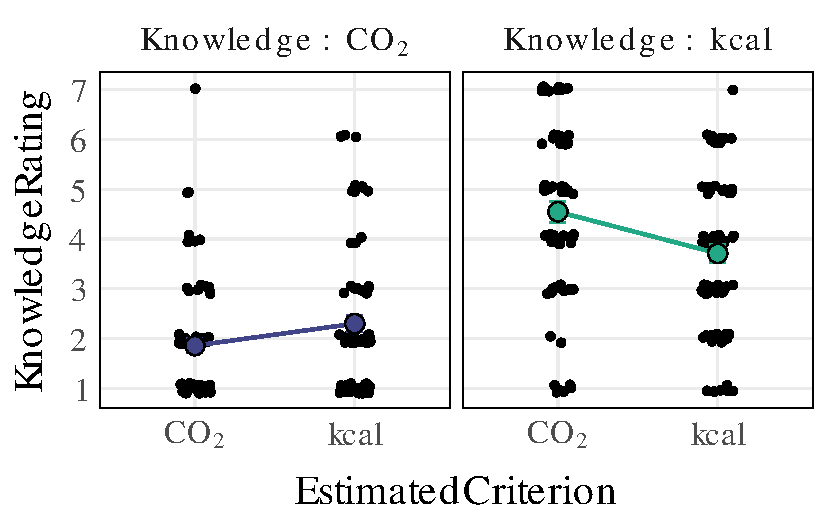
\includegraphics{supplement_files/figure-pdf/unnamed-chunk-3-1.pdf}

}

\caption{Figure S1. General knowledge ratings for C0\textsubscript{2}
footprint and calorie content of food items, depending on the estimated
criterion in the main task.}

\end{figure}%

\section{Number of Likes Posts}\label{number-of-likes-posts}

In the preregistration, we also predicted that a greater seeding effect
when participants saw more posts as indicated by the number of liked
posts. However, as already stated in the main text, almost all
participants liked every post, see the table below for the descriptive
statistics and the Figure S2 for the distribution of liked posts per
participant.

\begin{Shaded}
\begin{Highlighting}[]
\NormalTok{est }\SpecialCharTok{\%\textgreater{}\%} 
  \FunctionTok{select}\NormalTok{(ID,}\StringTok{"Account"}\OtherTok{=}\NormalTok{trained\_criterion,n\_posts\_liked) }\SpecialCharTok{\%\textgreater{}\%} 
  \FunctionTok{distinct}\NormalTok{() }\SpecialCharTok{\%\textgreater{}\%} 
  \FunctionTok{group\_by}\NormalTok{(Account) }\SpecialCharTok{\%\textgreater{}\%} 
  \FunctionTok{summarise}\NormalTok{(}\AttributeTok{m   =} \FunctionTok{mean}\NormalTok{(n\_posts\_liked),}
            \AttributeTok{sd  =} \FunctionTok{sd}\NormalTok{(n\_posts\_liked),}
            \AttributeTok{min =} \FunctionTok{min}\NormalTok{(n\_posts\_liked),}
            \AttributeTok{max =} \FunctionTok{max}\NormalTok{(n\_posts\_liked)) }\SpecialCharTok{\%\textgreater{}\%} 
  \FunctionTok{kbl}\NormalTok{(}\AttributeTok{col.names =} \FunctionTok{c}\NormalTok{(}\StringTok{"Account"}\NormalTok{,}\StringTok{"M"}\NormalTok{,}\StringTok{"SD"}\NormalTok{,}\StringTok{"Min"}\NormalTok{,}\StringTok{"Max"}\NormalTok{),}\AttributeTok{digits =} \DecValTok{2}\NormalTok{) }\SpecialCharTok{\%\textgreater{}\%} 
  \FunctionTok{kable\_paper}\NormalTok{()}
\end{Highlighting}
\end{Shaded}

\begin{table}
\centering
\begin{tabular}[t]{l|r|r|r|r}
\hline
Account & M & SD & Min & Max\\
\hline
CO2 & 29.25 & 1.58 & 21 & 30\\
\hline
Kcal & 28.55 & 4.48 & 1 & 30\\
\hline
\end{tabular}
\end{table}

\begin{Shaded}
\begin{Highlighting}[]
\NormalTok{est }\SpecialCharTok{\%\textgreater{}\%} 
  \FunctionTok{select}\NormalTok{(ID,trained\_criterion,est\_criterion,n\_posts\_liked) }\SpecialCharTok{\%\textgreater{}\%} 
  \FunctionTok{distinct}\NormalTok{() }\SpecialCharTok{\%\textgreater{}\%} 
  \FunctionTok{mutate}\NormalTok{(}\AttributeTok{trained\_criterion =} \FunctionTok{ifelse}\NormalTok{(trained\_criterion  }\SpecialCharTok{==} \StringTok{"CO2"}\NormalTok{,}\StringTok{"CO[2]"}\NormalTok{,}\StringTok{"kcal"}\NormalTok{)) }\SpecialCharTok{\%\textgreater{}\%} 
  \FunctionTok{ggplot}\NormalTok{(}\FunctionTok{aes}\NormalTok{(}\AttributeTok{x =}\NormalTok{ n\_posts\_liked,  }\AttributeTok{fill =}\NormalTok{ trained\_criterion)) }\SpecialCharTok{+}
    \FunctionTok{geom\_histogram}\NormalTok{(}\AttributeTok{alpha=}\FloatTok{0.75}\NormalTok{,}\AttributeTok{position =} \StringTok{"identity"}\NormalTok{,}\AttributeTok{bins=}\DecValTok{25}\NormalTok{) }\SpecialCharTok{+}
    \FunctionTok{scale\_fill\_manual}\NormalTok{(}\AttributeTok{values=}\FunctionTok{c}\NormalTok{(clrs[}\DecValTok{4}\NormalTok{],clrs[}\DecValTok{3}\NormalTok{]),}\AttributeTok{labels =} \FunctionTok{parse\_format}\NormalTok{()) }\SpecialCharTok{+}
    \FunctionTok{theme\_nice}\NormalTok{() }\SpecialCharTok{+}
    \FunctionTok{labs}\NormalTok{(}\AttributeTok{x    =} \StringTok{"Liked X out of 30 possible posts (15 seeding + 15 trivia facts)"}\NormalTok{,}
         \AttributeTok{y    =} \StringTok{"Frequency"}\NormalTok{,}
         \AttributeTok{fill =} \StringTok{"Account:"}\NormalTok{)}
\end{Highlighting}
\end{Shaded}

\begin{figure}[H]

{\centering 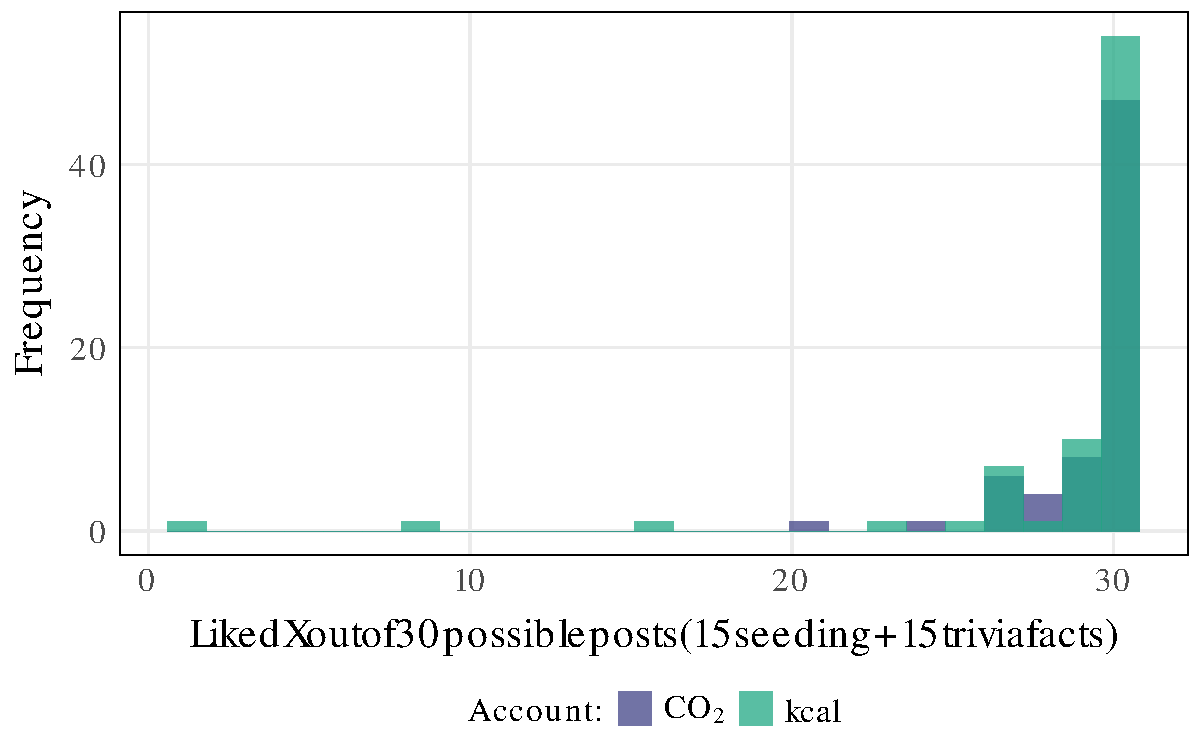
\includegraphics{supplement_files/figure-pdf/unnamed-chunk-5-1.pdf}

}

\caption{Figure S2. Distribution of number of liked posts per
participant.}

\end{figure}%

In addition, Figure S3 shows the scatter plots with the estimated
regression line when using the number of liked posts as an predictor of
OME or \(\rho\) (all \emph{p}s \textgreater{} 0.05)

\begin{Shaded}
\begin{Highlighting}[]
\NormalTok{est }\SpecialCharTok{\%\textgreater{}\%} 
 \FunctionTok{select}\NormalTok{(ID,trained\_criterion,est\_criterion,n\_posts\_liked, OME\_corr, rank\_z) }\SpecialCharTok{\%\textgreater{}\%} 
 \FunctionTok{group\_by}\NormalTok{(ID,trained\_criterion,est\_criterion) }\SpecialCharTok{\%\textgreater{}\%} 
 \FunctionTok{summarize}\NormalTok{(}\AttributeTok{OME    =} \FunctionTok{mean}\NormalTok{(OME\_corr),}
           \AttributeTok{rank\_z =} \FunctionTok{mean}\NormalTok{(rank\_z),}
           \AttributeTok{n\_posts\_liked =} \FunctionTok{mean}\NormalTok{(n\_posts\_liked),}
           \AttributeTok{.groups=}\StringTok{"drop"}\NormalTok{) }\SpecialCharTok{\%\textgreater{}\%} 
  \FunctionTok{mutate}\NormalTok{(}\AttributeTok{est\_criterion =} \FunctionTok{ifelse}\NormalTok{(est\_criterion }\SpecialCharTok{==} \StringTok{"CO2"}\NormalTok{,}
                                \StringTok{"bold(Estimated:\textasciitilde{}CO[2])"}\NormalTok{,}
                                \StringTok{"bold(Estimated:\textasciitilde{}kcal)"}\NormalTok{),}
         \AttributeTok{trained\_criterion =} \FunctionTok{ifelse}\NormalTok{(trained\_criterion }\SpecialCharTok{==} \StringTok{"CO2"}\NormalTok{,}
                                    \StringTok{"CO[2]"}\NormalTok{,}
                                    \StringTok{"kcal"}\NormalTok{)) }\SpecialCharTok{\%\textgreater{}\%} 
  \FunctionTok{rename}\NormalTok{(}\StringTok{\textasciigrave{}}\AttributeTok{Estimated Criterion}\StringTok{\textasciigrave{}} \OtherTok{=}\NormalTok{ est\_criterion,}
         \StringTok{\textasciigrave{}}\AttributeTok{Trained Criterion}\StringTok{\textasciigrave{}}   \OtherTok{=}\NormalTok{ trained\_criterion) }\SpecialCharTok{\%\textgreater{}\%} 
  \FunctionTok{pivot\_longer}\NormalTok{(}\AttributeTok{cols =} \FunctionTok{c}\NormalTok{(OME, rank\_z), }\AttributeTok{names\_to =} \StringTok{"DV"}\NormalTok{, }\AttributeTok{values\_to =} \StringTok{"val"}\NormalTok{) }\SpecialCharTok{\%\textgreater{}\%} 
  \FunctionTok{ggplot}\NormalTok{(}\FunctionTok{aes}\NormalTok{(}\AttributeTok{x =}\NormalTok{ n\_posts\_liked, }\AttributeTok{y =}\NormalTok{ val,}
             \AttributeTok{color =} \StringTok{\textasciigrave{}}\AttributeTok{Trained Criterion}\StringTok{\textasciigrave{}}\NormalTok{, }\AttributeTok{fill =} \StringTok{\textasciigrave{}}\AttributeTok{Trained Criterion}\StringTok{\textasciigrave{}}\NormalTok{)) }\SpecialCharTok{+}
    \FunctionTok{geom\_point}\NormalTok{(}\AttributeTok{shape=}\DecValTok{21}\NormalTok{,}\AttributeTok{color=}\StringTok{"black"}\NormalTok{, }\AttributeTok{alpha=}\NormalTok{.}\DecValTok{8}\NormalTok{) }\SpecialCharTok{+}
    \FunctionTok{geom\_smooth}\NormalTok{(}\AttributeTok{method=}\StringTok{"lm"}\NormalTok{,}\AttributeTok{fullrange=}\ConstantTok{TRUE}\NormalTok{,}\AttributeTok{alpha=}\FloatTok{0.1}\NormalTok{) }\SpecialCharTok{+}
    \FunctionTok{scale\_fill\_manual}\NormalTok{(}\AttributeTok{values=}\FunctionTok{c}\NormalTok{(clrs[}\DecValTok{4}\NormalTok{],clrs[}\DecValTok{3}\NormalTok{]),}\AttributeTok{labels =} \FunctionTok{parse\_format}\NormalTok{()) }\SpecialCharTok{+}
    \FunctionTok{scale\_color\_manual}\NormalTok{(}\AttributeTok{values=}\FunctionTok{c}\NormalTok{(clrs[}\DecValTok{4}\NormalTok{],clrs[}\DecValTok{3}\NormalTok{]),}\AttributeTok{labels =} \FunctionTok{parse\_format}\NormalTok{()) }\SpecialCharTok{+}
    \FunctionTok{facet\_grid}\NormalTok{(DV}\SpecialCharTok{\textasciitilde{}}\StringTok{\textasciigrave{}}\AttributeTok{Estimated Criterion}\StringTok{\textasciigrave{}}\NormalTok{,}\AttributeTok{labeller =}\NormalTok{ label\_parsed) }\SpecialCharTok{+}
    \FunctionTok{labs}\NormalTok{(}\AttributeTok{fill  =} \StringTok{"Trained Criterion"}\NormalTok{, }
         \AttributeTok{y     =} \StringTok{"Dependet Variable"}\NormalTok{,}
         \AttributeTok{x     =} \StringTok{"Number of liked posts"}\NormalTok{) }\SpecialCharTok{+}
    \FunctionTok{theme\_nice}\NormalTok{()}
\end{Highlighting}
\end{Shaded}

\begin{figure}[H]

{\centering 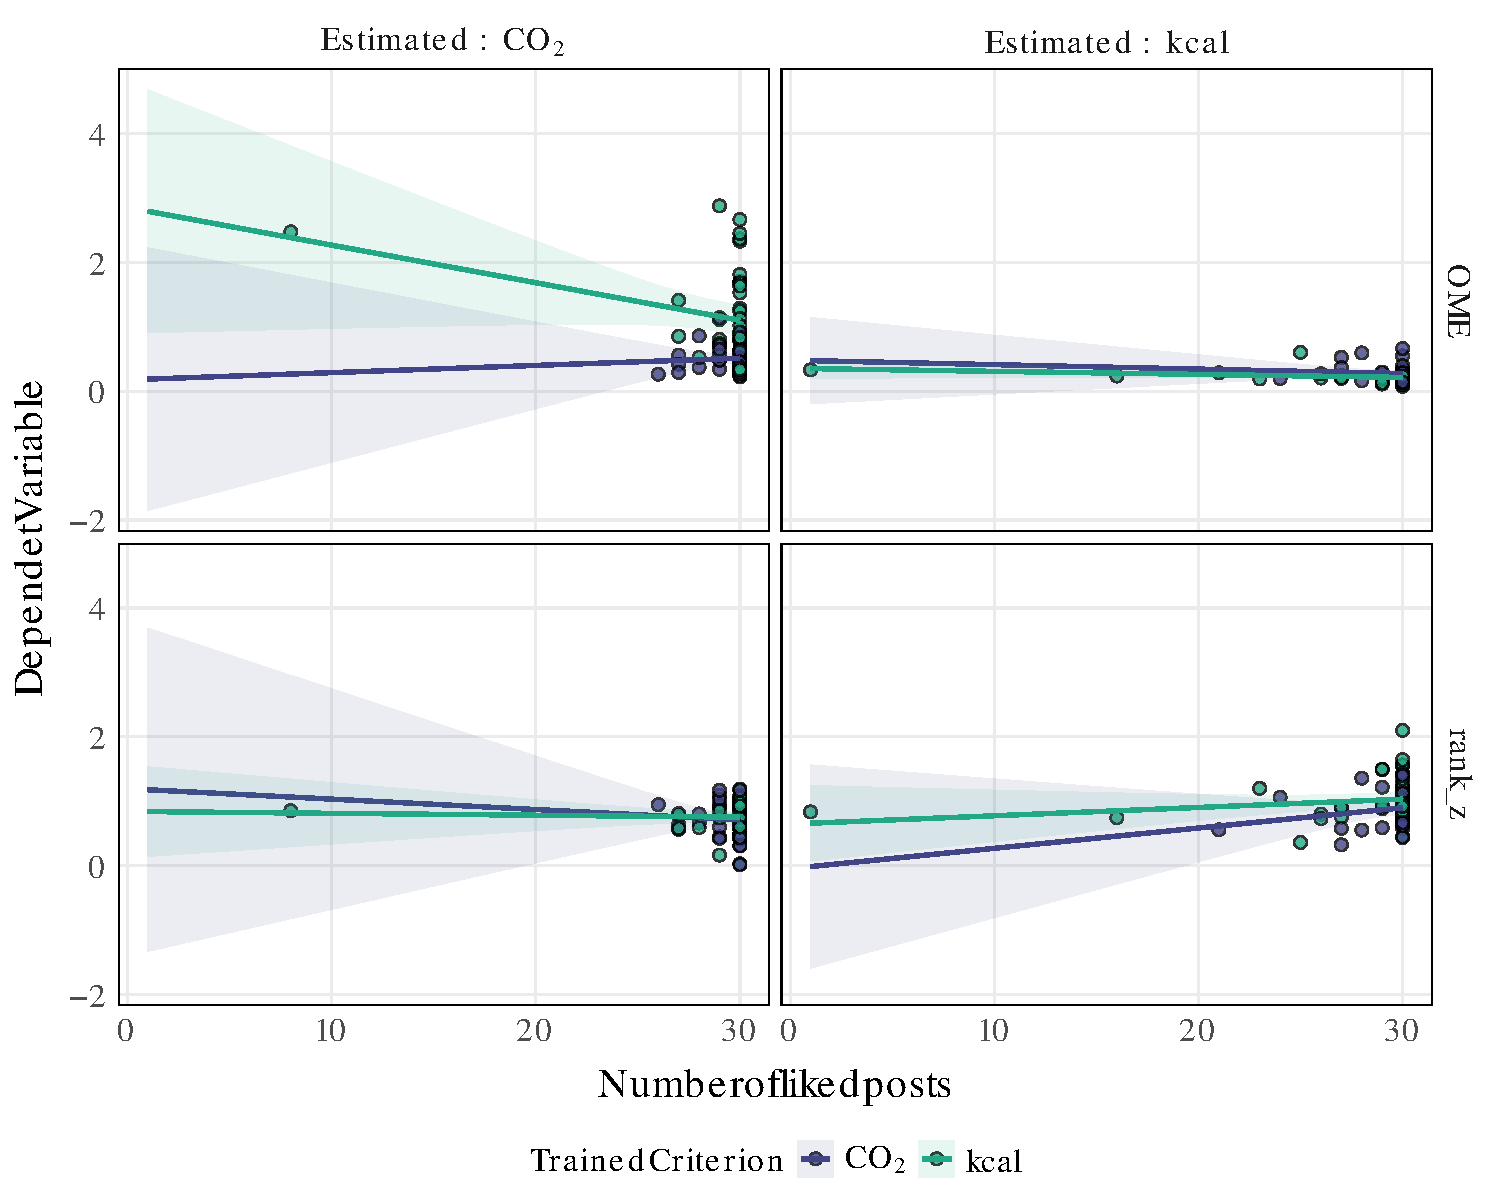
\includegraphics{supplement_files/figure-pdf/unnamed-chunk-6-1.pdf}

}

\caption{Figure S3. Relationship of number of liked posts and OME/rank
correlation (z-transformed) per trained and estimated criterion}

\end{figure}%

\section{Detailed Modeling Results}\label{detailed-modeling-results}

Here we provide for all models reported in the main manuscript more
detailed modeling results, including a table with the mean, standard
deviation, 95\%-HDI, effective sample size (ESS) and \(\hat{R}\) for
each estimated parameter (random and fixed), as well as figures showing
the MCMC-traces for the main fixed effects parameters (intercept and
effect parameter) and posterior predictive distributions of the complete
model.

\subsection{Hypothesis 1a (OME)}\label{hypothesis-1a-ome}

\subsubsection{\texorpdfstring{CO\textsubscript{2}
M0}{CO2 M0}}\label{co2-m0}

\begin{Shaded}
\begin{Highlighting}[]
\CommentTok{\# Load model }
\NormalTok{temp }\OtherTok{\textless{}{-}} \FunctionTok{brm}\NormalTok{(}\AttributeTok{file=}\StringTok{"../Results/fit\_H1a\_CO2\_M0.rds"}\NormalTok{)}

\CommentTok{\# Print Formular}
\NormalTok{temp}\SpecialCharTok{$}\NormalTok{formula}
\end{Highlighting}
\end{Shaded}

\begin{verbatim}
OME_corr ~ 1 + (1 | ID) + (match_domain | ID_item) 
\end{verbatim}

\begin{Shaded}
\begin{Highlighting}[]
\CommentTok{\# Make model parameter table}
\FunctionTok{model\_parameters}\NormalTok{(temp, }\AttributeTok{centrality =} \StringTok{"mean"}\NormalTok{, }\AttributeTok{dispersion =} \ConstantTok{TRUE}\NormalTok{, }
                 \AttributeTok{ci\_method =} \StringTok{"hdi"}\NormalTok{, }\AttributeTok{effects =} \StringTok{"all"}\NormalTok{) }\SpecialCharTok{\%\textgreater{}\%} 
  \FunctionTok{kable}\NormalTok{(}\AttributeTok{digits=}\DecValTok{2}\NormalTok{) }\SpecialCharTok{\%\textgreater{}\%} \FunctionTok{kable\_paper}\NormalTok{()}
\end{Highlighting}
\end{Shaded}

\begin{longtable*}[t]{lllrrrrrrrrl}
\toprule
Parameter & Effects & Component & Mean & SD & CI & CI\_low & CI\_high & pd & Rhat & ESS & Group\\
\midrule
b\_Intercept & fixed & conditional & -0.63 & 0.10 & 0.95 & -0.83 & -0.42 & 1 & 1 & 2952.33 & \\
sd\_ID\_\_Intercept & random & conditional & 0.80 & 0.07 & 0.95 & 0.67 & 0.94 & 1 & 1 & 4688.51 & ID\\
sd\_ID\_item\_\_Intercept & random & conditional & 0.33 & 0.03 & 0.95 & 0.26 & 0.40 & 1 & 1 & 10120.97 & ID\_item\\
sd\_ID\_item\_\_match\_domain & random & conditional & 0.20 & 0.04 & 0.95 & 0.13 & 0.28 & 1 & 1 & 20100.90 & ID\_item\\
cor\_ID\_item\_\_Intercept\_\_match\_domain & random & conditional & 0.81 & 0.12 & 0.95 & 0.57 & 0.99 & 1 & 1 & 19283.57 & ID\_item\\
\addlinespace
sigma & fixed & sigma & 0.88 & 0.01 & 0.95 & 0.86 & 0.90 & 1 & 1 & 50236.69 & \\
\bottomrule
\end{longtable*}

\begin{Shaded}
\begin{Highlighting}[]
\CommentTok{\# Make trace and pp{-}check plot}
\FunctionTok{brms\_plot}\NormalTok{(temp)}
\end{Highlighting}
\end{Shaded}

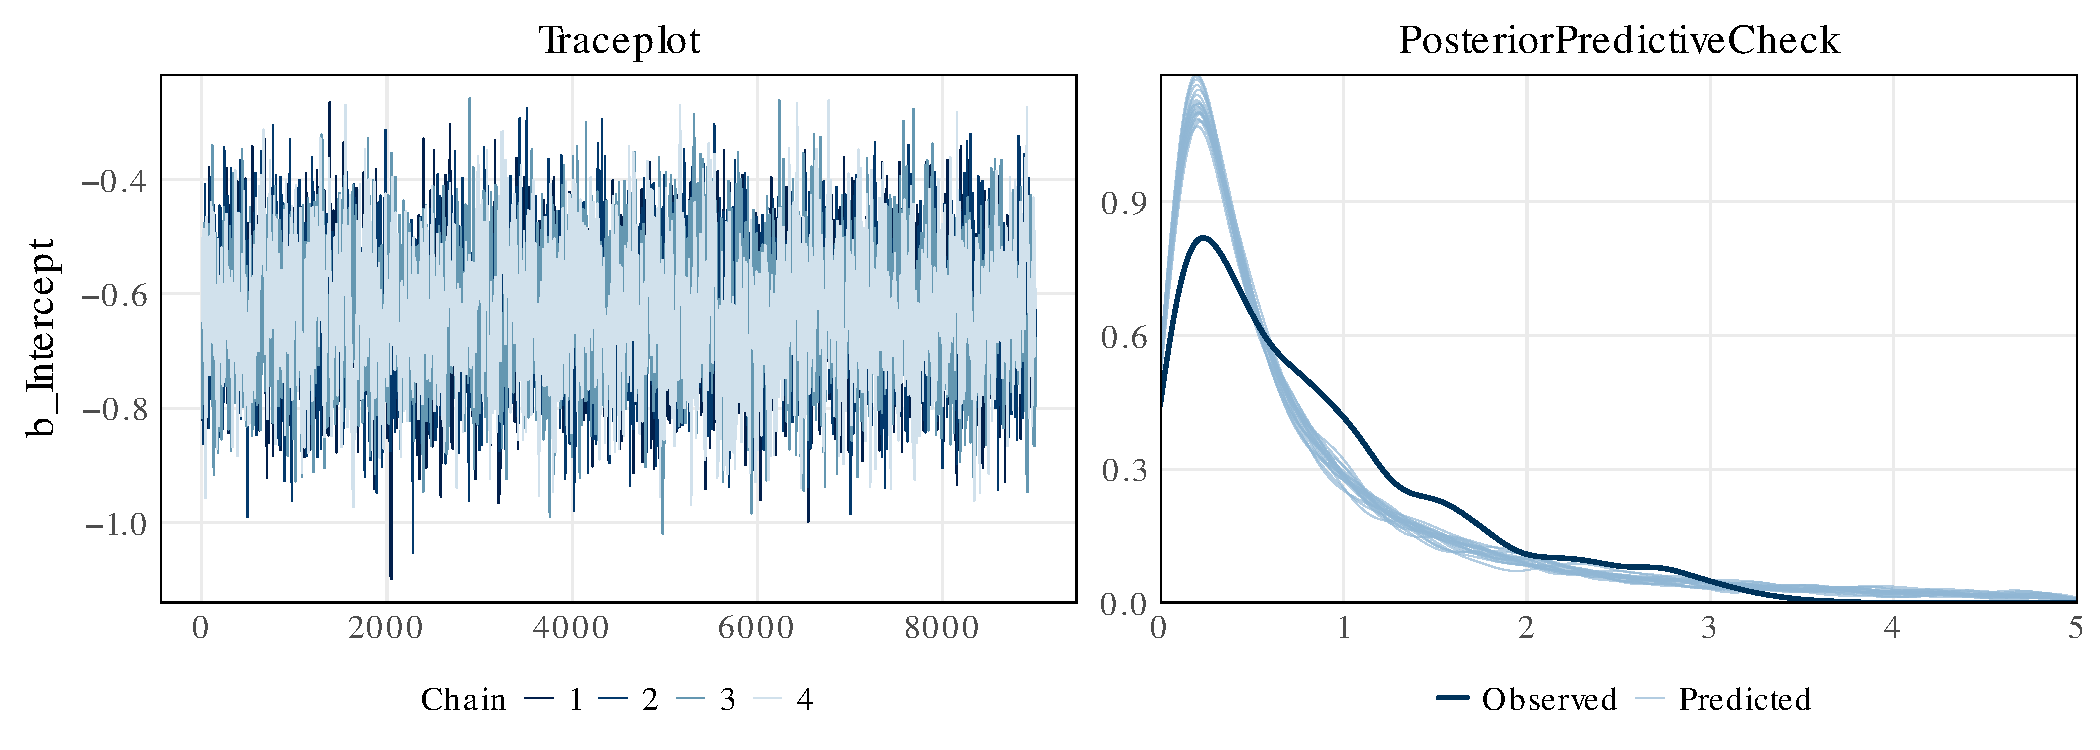
\includegraphics{supplement_files/figure-pdf/h1aM0CO2-1.pdf}

\subsubsection{\texorpdfstring{CO\textsubscript{2}
M1}{CO2 M1}}\label{co2-m1}

\begin{Shaded}
\begin{Highlighting}[]
\CommentTok{\# Load model }
\NormalTok{temp }\OtherTok{\textless{}{-}} \FunctionTok{brm}\NormalTok{(}\AttributeTok{file=}\StringTok{"../Results/fit\_H1a\_CO2\_M1.rds"}\NormalTok{)}

\CommentTok{\# Print Formular}
\NormalTok{temp}\SpecialCharTok{$}\NormalTok{formula}
\end{Highlighting}
\end{Shaded}

\begin{verbatim}
OME_corr ~ match_domain + (1 | ID) + (match_domain | ID_item) 
\end{verbatim}

\begin{Shaded}
\begin{Highlighting}[]
\CommentTok{\# Make model parameter table}
\FunctionTok{model\_parameters}\NormalTok{(temp, }\AttributeTok{centrality =} \StringTok{"mean"}\NormalTok{, }\AttributeTok{dispersion =} \ConstantTok{TRUE}\NormalTok{, }
                 \AttributeTok{ci\_method =} \StringTok{"hdi"}\NormalTok{, }\AttributeTok{effects =} \StringTok{"all"}\NormalTok{) }\SpecialCharTok{\%\textgreater{}\%} 
  \FunctionTok{kable}\NormalTok{(}\AttributeTok{digits=}\DecValTok{2}\NormalTok{) }\SpecialCharTok{\%\textgreater{}\%} \FunctionTok{kable\_paper}\NormalTok{()}
\end{Highlighting}
\end{Shaded}

\begin{longtable*}[t]{lllrrrrrrrrl}
\toprule
Parameter & Effects & Component & Mean & SD & CI & CI\_low & CI\_high & pd & Rhat & ESS & Group\\
\midrule
b\_Intercept & fixed & conditional & -0.68 & 0.09 & 0.95 & -0.87 & -0.50 & 1 & 1 & 4760.12 & \\
b\_match\_domain & fixed & conditional & -0.67 & 0.18 & 0.95 & -1.03 & -0.32 & 1 & 1 & 3283.60 & \\
sd\_ID\_\_Intercept & random & conditional & 0.70 & 0.06 & 0.95 & 0.58 & 0.82 & 1 & 1 & 6443.01 & ID\\
sd\_ID\_item\_\_Intercept & random & conditional & 0.33 & 0.03 & 0.95 & 0.26 & 0.40 & 1 & 1 & 10574.83 & ID\_item\\
sd\_ID\_item\_\_match\_domain & random & conditional & 0.20 & 0.04 & 0.95 & 0.13 & 0.27 & 1 & 1 & 23835.70 & ID\_item\\
\addlinespace
cor\_ID\_item\_\_Intercept\_\_match\_domain & random & conditional & 0.81 & 0.12 & 0.95 & 0.57 & 0.99 & 1 & 1 & 21153.55 & ID\_item\\
sigma & fixed & sigma & 0.88 & 0.01 & 0.95 & 0.86 & 0.90 & 1 & 1 & 63425.68 & \\
\bottomrule
\end{longtable*}

\begin{Shaded}
\begin{Highlighting}[]
\CommentTok{\# Make trace and pp{-}check plot}
\FunctionTok{brms\_plot}\NormalTok{(temp)  }\SpecialCharTok{+} \FunctionTok{plot\_layout}\NormalTok{(}\AttributeTok{widths =} \FunctionTok{c}\NormalTok{(}\DecValTok{2}\NormalTok{, }\DecValTok{1}\NormalTok{))}
\end{Highlighting}
\end{Shaded}

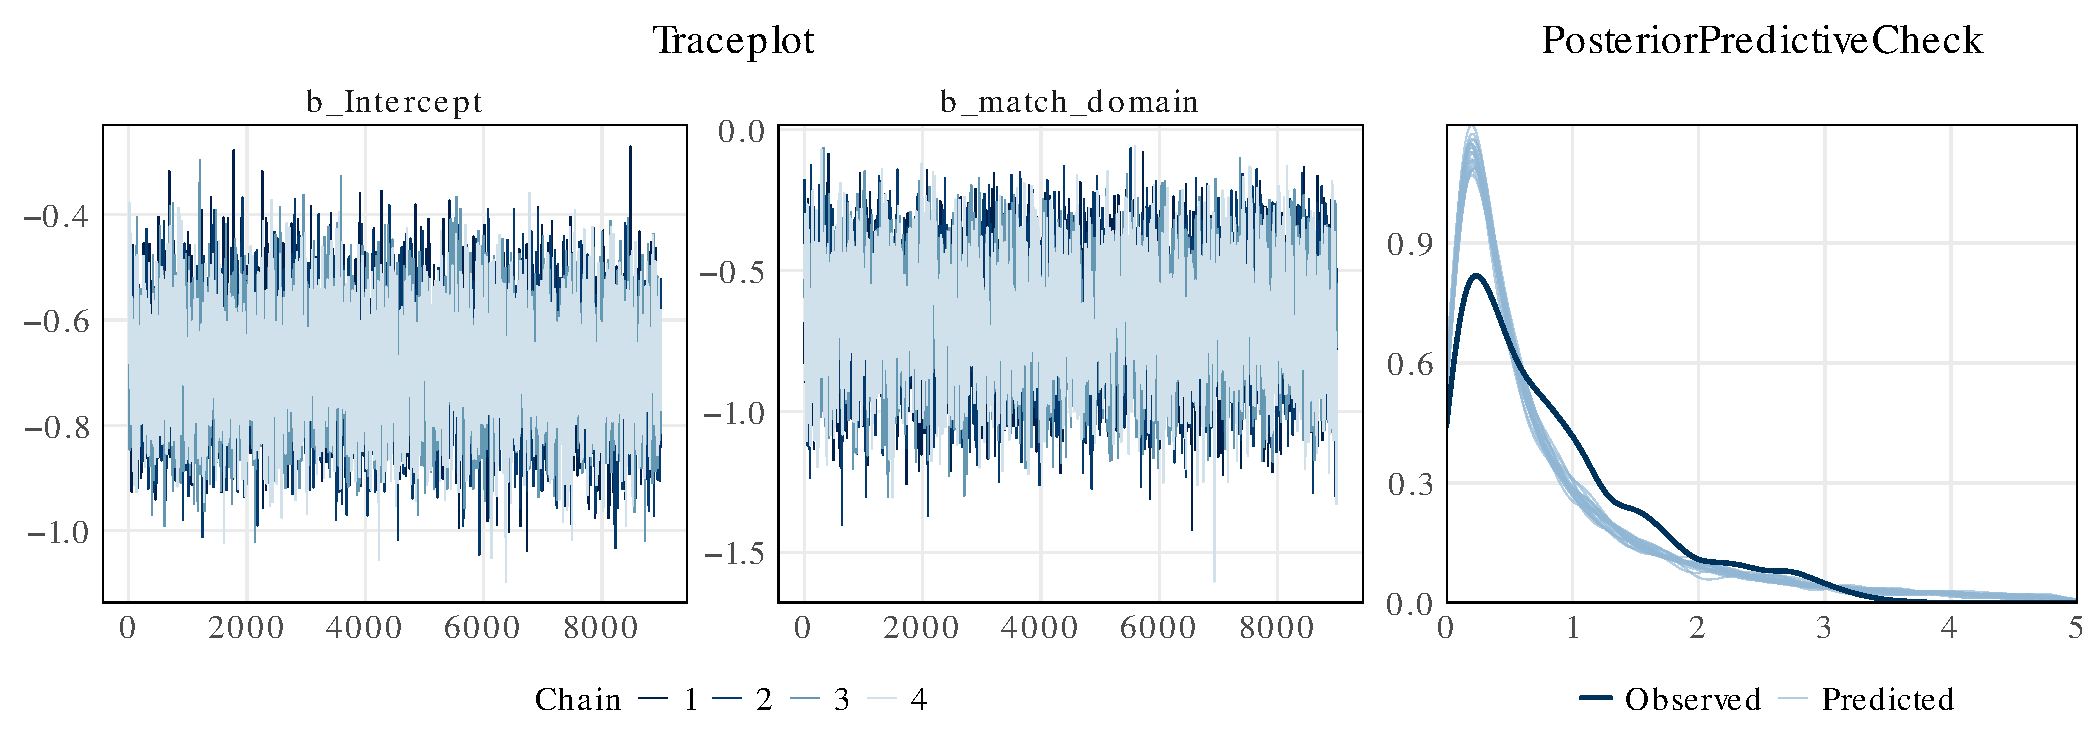
\includegraphics{supplement_files/figure-pdf/h1aM1CO2-1.pdf}

\subsubsection{kcal M0}\label{kcal-m0}

\begin{Shaded}
\begin{Highlighting}[]
\CommentTok{\# Load model }
\NormalTok{temp }\OtherTok{\textless{}{-}} \FunctionTok{brm}\NormalTok{(}\AttributeTok{file=}\StringTok{"../Results/fit\_H1a\_kcal\_M0.rds"}\NormalTok{)}

\CommentTok{\# Print Formular}
\NormalTok{temp}\SpecialCharTok{$}\NormalTok{formula}
\end{Highlighting}
\end{Shaded}

\begin{verbatim}
OME_corr ~ 1 + (1 | ID) + (match_domain | ID_item) 
\end{verbatim}

\begin{Shaded}
\begin{Highlighting}[]
\CommentTok{\# Make model parameter table}
\FunctionTok{model\_parameters}\NormalTok{(temp, }\AttributeTok{centrality =} \StringTok{"mean"}\NormalTok{, }\AttributeTok{dispersion =} \ConstantTok{TRUE}\NormalTok{, }
                 \AttributeTok{ci\_method =} \StringTok{"hdi"}\NormalTok{, }\AttributeTok{effects =} \StringTok{"all"}\NormalTok{) }\SpecialCharTok{\%\textgreater{}\%} 
  \FunctionTok{kable}\NormalTok{(}\AttributeTok{digits=}\DecValTok{2}\NormalTok{) }\SpecialCharTok{\%\textgreater{}\%} \FunctionTok{kable\_paper}\NormalTok{()}
\end{Highlighting}
\end{Shaded}

\begin{longtable*}[t]{lllrrrrrrrrl}
\toprule
Parameter & Effects & Component & Mean & SD & CI & CI\_low & CI\_high & pd & Rhat & ESS & Group\\
\midrule
b\_Intercept & fixed & conditional & -1.90 & 0.07 & 0.95 & -2.04 & -1.76 & 1.00 & 1 & 6942.96 & \\
sd\_ID\_\_Intercept & random & conditional & 0.44 & 0.04 & 0.95 & 0.36 & 0.53 & 1.00 & 1 & 9638.45 & ID\\
sd\_ID\_item\_\_Intercept & random & conditional & 0.35 & 0.04 & 0.95 & 0.28 & 0.43 & 1.00 & 1 & 11449.45 & ID\_item\\
sd\_ID\_item\_\_match\_domain & random & conditional & 0.13 & 0.03 & 0.95 & 0.07 & 0.20 & 1.00 & 1 & 29752.77 & ID\_item\\
cor\_ID\_item\_\_Intercept\_\_match\_domain & random & conditional & 0.08 & 0.35 & 0.95 & -0.61 & 0.75 & 0.59 & 1 & 31297.43 & ID\_item\\
\addlinespace
sigma & fixed & sigma & 1.19 & 0.01 & 0.95 & 1.17 & 1.22 & 1.00 & 1 & 54617.30 & \\
\bottomrule
\end{longtable*}

\begin{Shaded}
\begin{Highlighting}[]
\CommentTok{\# Make trace and pp{-}check plot}
\FunctionTok{brms\_plot}\NormalTok{(temp)}
\end{Highlighting}
\end{Shaded}

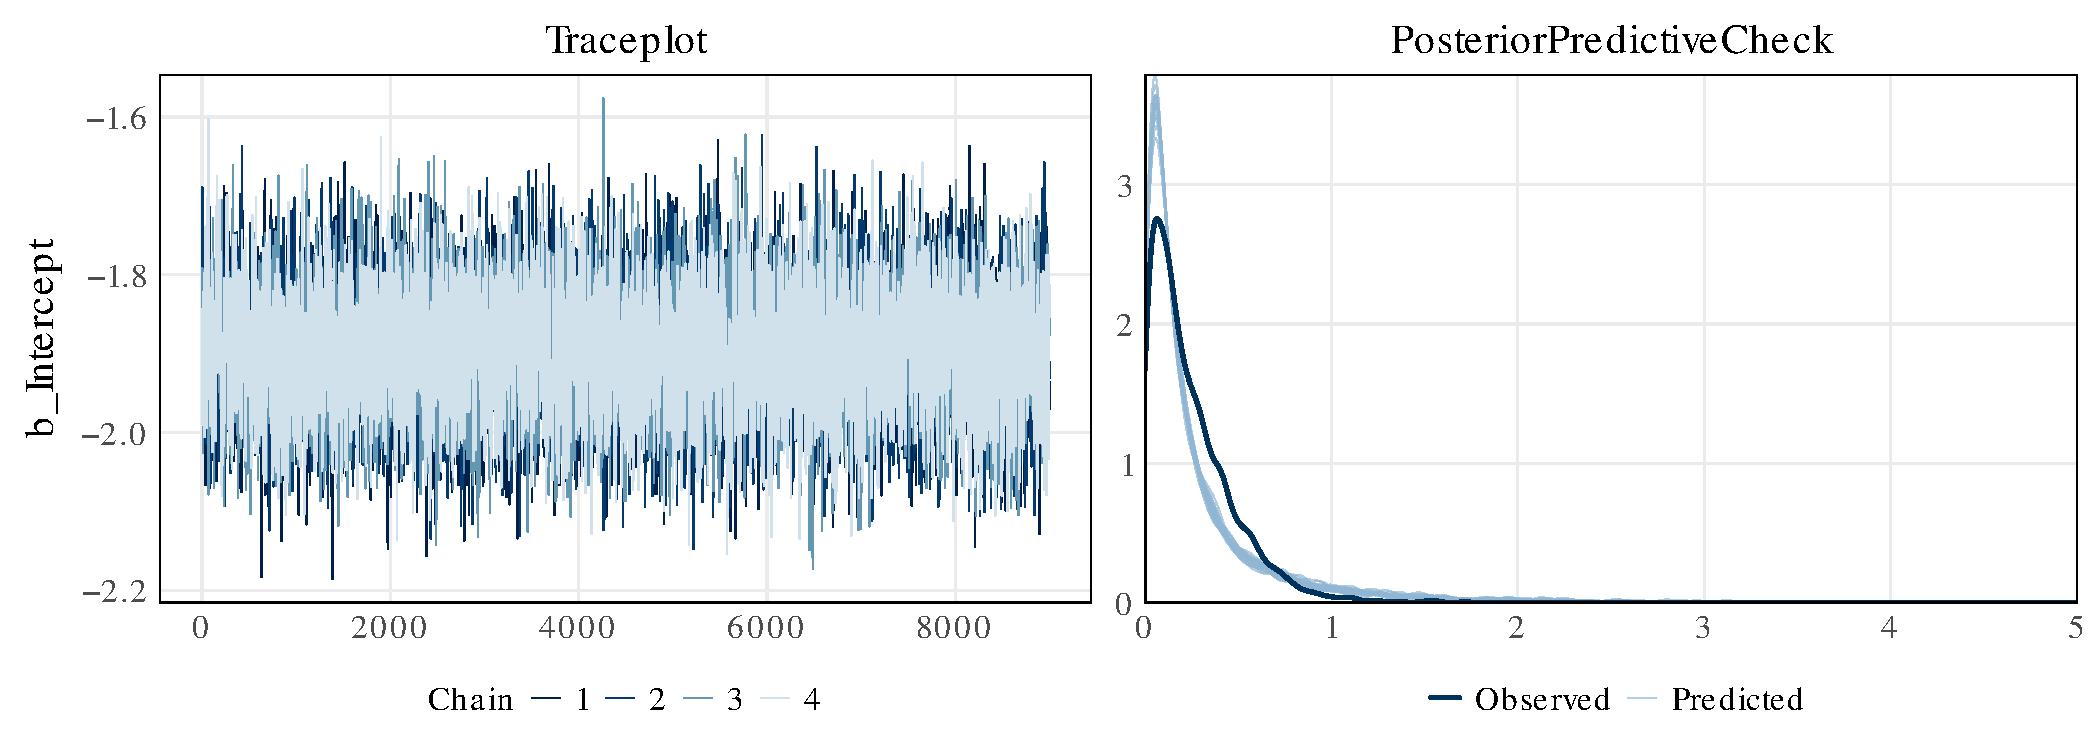
\includegraphics{supplement_files/figure-pdf/h1aM0kcal-1.pdf}

\subsubsection{kcal M1}\label{kcal-m1}

\begin{Shaded}
\begin{Highlighting}[]
\CommentTok{\# Load model }
\NormalTok{temp }\OtherTok{\textless{}{-}} \FunctionTok{brm}\NormalTok{(}\AttributeTok{file=}\StringTok{"../Results/fit\_H1a\_kcal\_M1.rds"}\NormalTok{)}

\CommentTok{\# Print Formular}
\NormalTok{temp}\SpecialCharTok{$}\NormalTok{formula}
\end{Highlighting}
\end{Shaded}

\begin{verbatim}
OME_corr ~ match_domain + (1 | ID) + (match_domain | ID_item) 
\end{verbatim}

\begin{Shaded}
\begin{Highlighting}[]
\CommentTok{\# Make model parameter table}
\FunctionTok{model\_parameters}\NormalTok{(temp, }\AttributeTok{centrality =} \StringTok{"mean"}\NormalTok{, }\AttributeTok{dispersion =} \ConstantTok{TRUE}\NormalTok{, }
                 \AttributeTok{ci\_method =} \StringTok{"hdi"}\NormalTok{, }\AttributeTok{effects =} \StringTok{"all"}\NormalTok{) }\SpecialCharTok{\%\textgreater{}\%} 
  \FunctionTok{kable}\NormalTok{(}\AttributeTok{digits=}\DecValTok{2}\NormalTok{) }\SpecialCharTok{\%\textgreater{}\%} \FunctionTok{kable\_paper}\NormalTok{()}
\end{Highlighting}
\end{Shaded}

\begin{longtable*}[t]{lllrrrrrrrrl}
\toprule
Parameter & Effects & Component & Mean & SD & CI & CI\_low & CI\_high & pd & Rhat & ESS & Group\\
\midrule
b\_Intercept & fixed & conditional & -1.90 & 0.07 & 0.95 & -2.04 & -1.76 & 1.00 & 1 & 6572.61 & \\
b\_match\_domain & fixed & conditional & -0.19 & 0.09 & 0.95 & -0.37 & -0.01 & 0.98 & 1 & 11324.63 & \\
sd\_ID\_\_Intercept & random & conditional & 0.43 & 0.04 & 0.95 & 0.36 & 0.52 & 1.00 & 1 & 10312.15 & ID\\
sd\_ID\_item\_\_Intercept & random & conditional & 0.35 & 0.04 & 0.95 & 0.27 & 0.43 & 1.00 & 1 & 11160.42 & ID\_item\\
sd\_ID\_item\_\_match\_domain & random & conditional & 0.13 & 0.03 & 0.95 & 0.07 & 0.20 & 1.00 & 1 & 30257.64 & ID\_item\\
\addlinespace
cor\_ID\_item\_\_Intercept\_\_match\_domain & random & conditional & 0.05 & 0.36 & 0.95 & -0.64 & 0.73 & 0.56 & 1 & 33234.07 & ID\_item\\
sigma & fixed & sigma & 1.19 & 0.02 & 0.95 & 1.17 & 1.22 & 1.00 & 1 & 47187.67 & \\
\bottomrule
\end{longtable*}

\begin{Shaded}
\begin{Highlighting}[]
\CommentTok{\# Make trace and pp{-}check plot}
\FunctionTok{brms\_plot}\NormalTok{(temp)  }\SpecialCharTok{+} \FunctionTok{plot\_layout}\NormalTok{(}\AttributeTok{widths =} \FunctionTok{c}\NormalTok{(}\DecValTok{2}\NormalTok{, }\DecValTok{1}\NormalTok{))}
\end{Highlighting}
\end{Shaded}

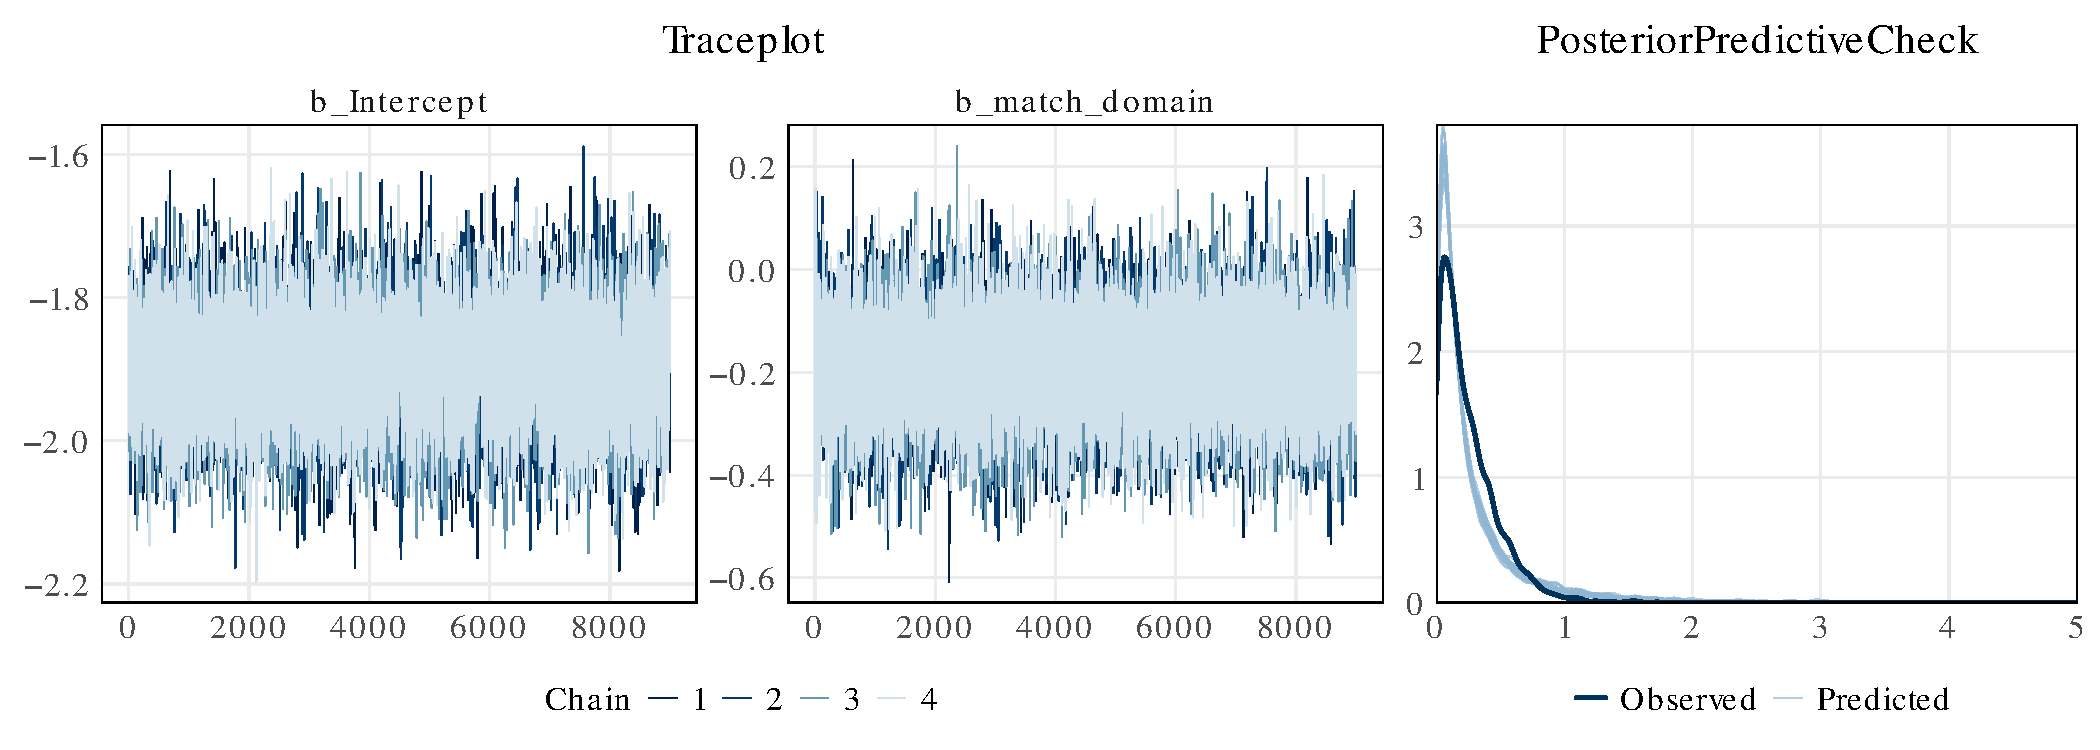
\includegraphics{supplement_files/figure-pdf/h1aM1kcal-1.pdf}

\subsection{\texorpdfstring{Hypothesis 1b
(\(\rho\))}{Hypothesis 1b (\textbackslash rho)}}\label{hypothesis-1b-rho}

\subsubsection{\texorpdfstring{CO\textsubscript{2}
M0}{CO2 M0}}\label{co2-m0-1}

\begin{Shaded}
\begin{Highlighting}[]
\CommentTok{\# Load model }
\NormalTok{temp }\OtherTok{\textless{}{-}} \FunctionTok{brm}\NormalTok{(}\AttributeTok{file=}\StringTok{"../Results/fit\_H1b\_CO2\_M0.rds"}\NormalTok{)}

\CommentTok{\# Print Formular}
\NormalTok{temp}\SpecialCharTok{$}\NormalTok{formula}
\end{Highlighting}
\end{Shaded}

\begin{verbatim}
rank_z ~ 1 + (1 | ID) 
\end{verbatim}

\begin{Shaded}
\begin{Highlighting}[]
\CommentTok{\# Make model parameter table}
\FunctionTok{model\_parameters}\NormalTok{(temp, }\AttributeTok{centrality =} \StringTok{"mean"}\NormalTok{, }\AttributeTok{dispersion =} \ConstantTok{TRUE}\NormalTok{, }
                 \AttributeTok{ci\_method =} \StringTok{"hdi"}\NormalTok{, }\AttributeTok{effects =} \StringTok{"all"}\NormalTok{) }\SpecialCharTok{\%\textgreater{}\%} 
  \FunctionTok{kable}\NormalTok{(}\AttributeTok{digits=}\DecValTok{2}\NormalTok{) }\SpecialCharTok{\%\textgreater{}\%} \FunctionTok{kable\_paper}\NormalTok{()}
\end{Highlighting}
\end{Shaded}

\begin{longtable*}[t]{lllrrrrrrrrl}
\toprule
Parameter & Effects & Component & Mean & SD & CI & CI\_low & CI\_high & pd & Rhat & ESS & Group\\
\midrule
b\_Intercept & fixed & conditional & 0.71 & 0.03 & 0.95 & 0.64 & 0.77 & 1 & 1 & 15250.74 & \\
sd\_ID\_\_Intercept & random & conditional & 0.19 & 0.05 & 0.95 & 0.10 & 0.29 & 1 & 1 & 1795.40 & ID\\
sigma & fixed & sigma & 0.19 & 0.05 & 0.95 & 0.10 & 0.28 & 1 & 1 & 1270.07 & \\
\bottomrule
\end{longtable*}

\begin{Shaded}
\begin{Highlighting}[]
\CommentTok{\# Make trace and pp{-}check plot}
\FunctionTok{brms\_plot}\NormalTok{(temp,}\AttributeTok{lim=}\FunctionTok{c}\NormalTok{(}\SpecialCharTok{{-}}\DecValTok{1}\NormalTok{,}\DecValTok{3}\NormalTok{))}
\end{Highlighting}
\end{Shaded}

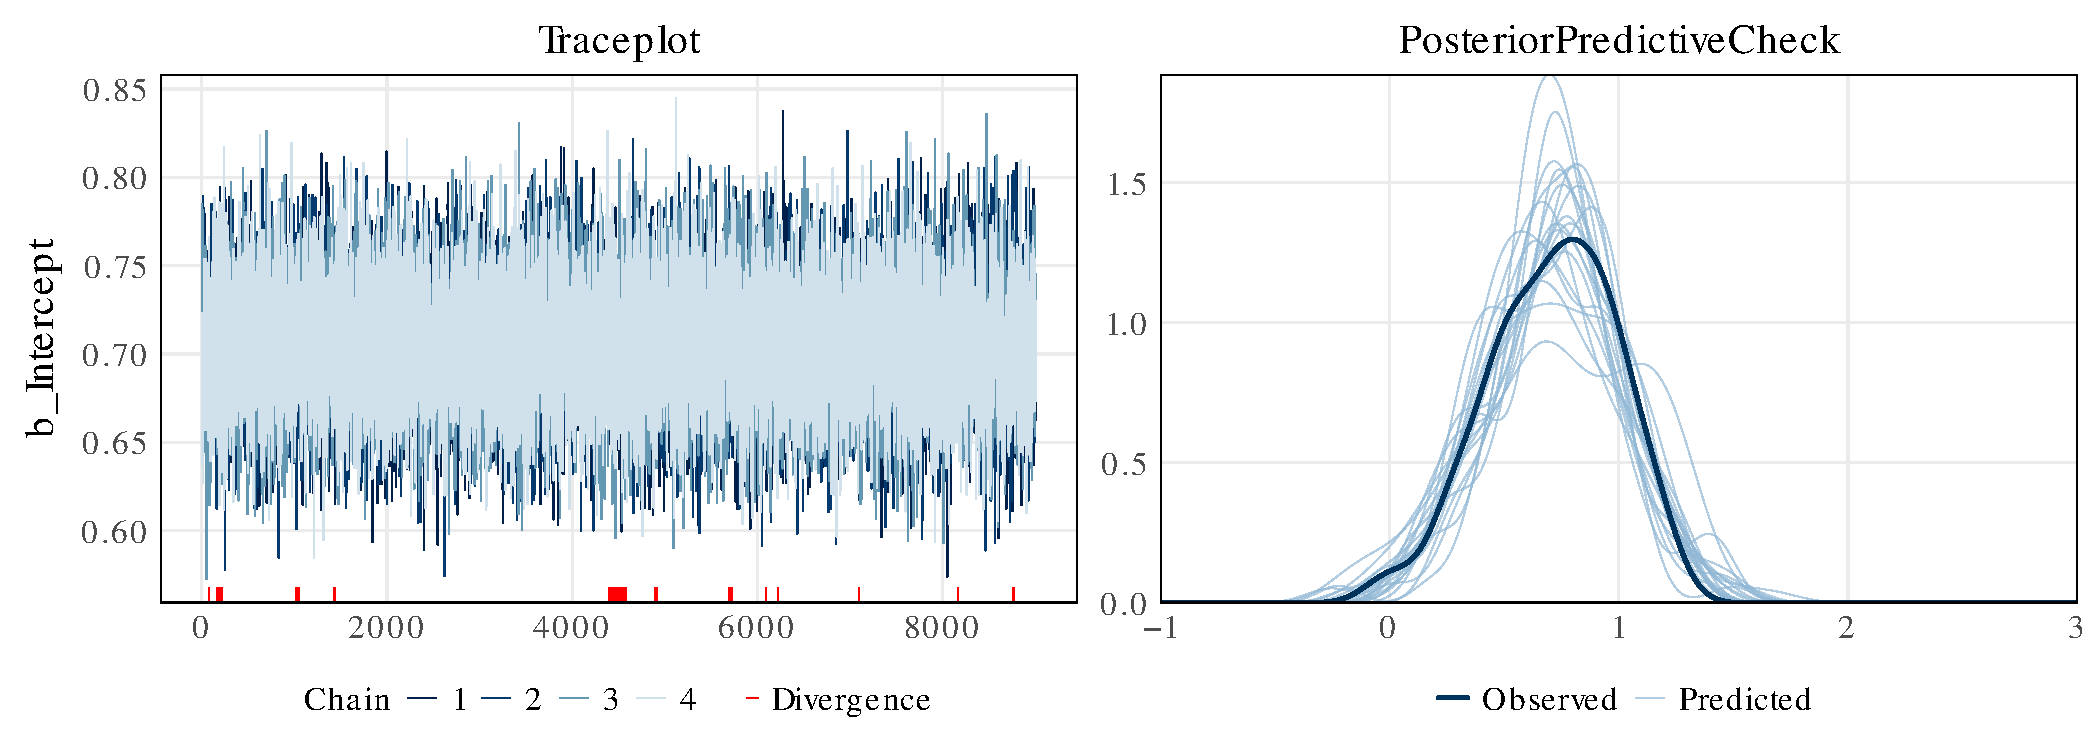
\includegraphics{supplement_files/figure-pdf/h1bM0CO2-1.pdf}

\subsubsection{\texorpdfstring{CO\textsubscript{2}
M1}{CO2 M1}}\label{co2-m1-1}

\begin{Shaded}
\begin{Highlighting}[]
\CommentTok{\# Load model }
\NormalTok{temp }\OtherTok{\textless{}{-}} \FunctionTok{brm}\NormalTok{(}\AttributeTok{file=}\StringTok{"../Results/fit\_H1b\_CO2\_M1.rds"}\NormalTok{)}

\CommentTok{\# Print Formular}
\NormalTok{temp}\SpecialCharTok{$}\NormalTok{formula}
\end{Highlighting}
\end{Shaded}

\begin{verbatim}
rank_z ~ match_domain + (1 | ID) 
\end{verbatim}

\begin{Shaded}
\begin{Highlighting}[]
\CommentTok{\# Make model parameter table}
\FunctionTok{model\_parameters}\NormalTok{(temp, }\AttributeTok{centrality =} \StringTok{"mean"}\NormalTok{, }\AttributeTok{dispersion =} \ConstantTok{TRUE}\NormalTok{, }
                 \AttributeTok{ci\_method =} \StringTok{"hdi"}\NormalTok{, }\AttributeTok{effects =} \StringTok{"all"}\NormalTok{) }\SpecialCharTok{\%\textgreater{}\%} 
  \FunctionTok{kable}\NormalTok{(}\AttributeTok{digits=}\DecValTok{2}\NormalTok{) }\SpecialCharTok{\%\textgreater{}\%} \FunctionTok{kable\_paper}\NormalTok{()}
\end{Highlighting}
\end{Shaded}

\begin{longtable*}[t]{lllrrrrrrrrl}
\toprule
Parameter & Effects & Component & Mean & SD & CI & CI\_low & CI\_high & pd & Rhat & ESS & Group\\
\midrule
b\_Intercept & fixed & conditional & 0.71 & 0.03 & 0.95 & 0.64 & 0.77 & 1.00 & 1 & 20663.28 & \\
b\_match\_domain & fixed & conditional & 0.01 & 0.07 & 0.95 & -0.12 & 0.14 & 0.55 & 1 & 20138.30 & \\
sd\_ID\_\_Intercept & random & conditional & 0.19 & 0.05 & 0.95 & 0.10 & 0.28 & 1.00 & 1 & 2315.68 & ID\\
sigma & fixed & sigma & 0.20 & 0.05 & 0.95 & 0.10 & 0.28 & 1.00 & 1 & 1868.11 & \\
\bottomrule
\end{longtable*}

\begin{Shaded}
\begin{Highlighting}[]
\CommentTok{\# Make trace and pp{-}check plot}
\FunctionTok{brms\_plot}\NormalTok{(temp,}\AttributeTok{lim=}\FunctionTok{c}\NormalTok{(}\SpecialCharTok{{-}}\DecValTok{1}\NormalTok{,}\DecValTok{3}\NormalTok{))  }\SpecialCharTok{+} \FunctionTok{plot\_layout}\NormalTok{(}\AttributeTok{widths =} \FunctionTok{c}\NormalTok{(}\DecValTok{2}\NormalTok{, }\DecValTok{1}\NormalTok{))}
\end{Highlighting}
\end{Shaded}

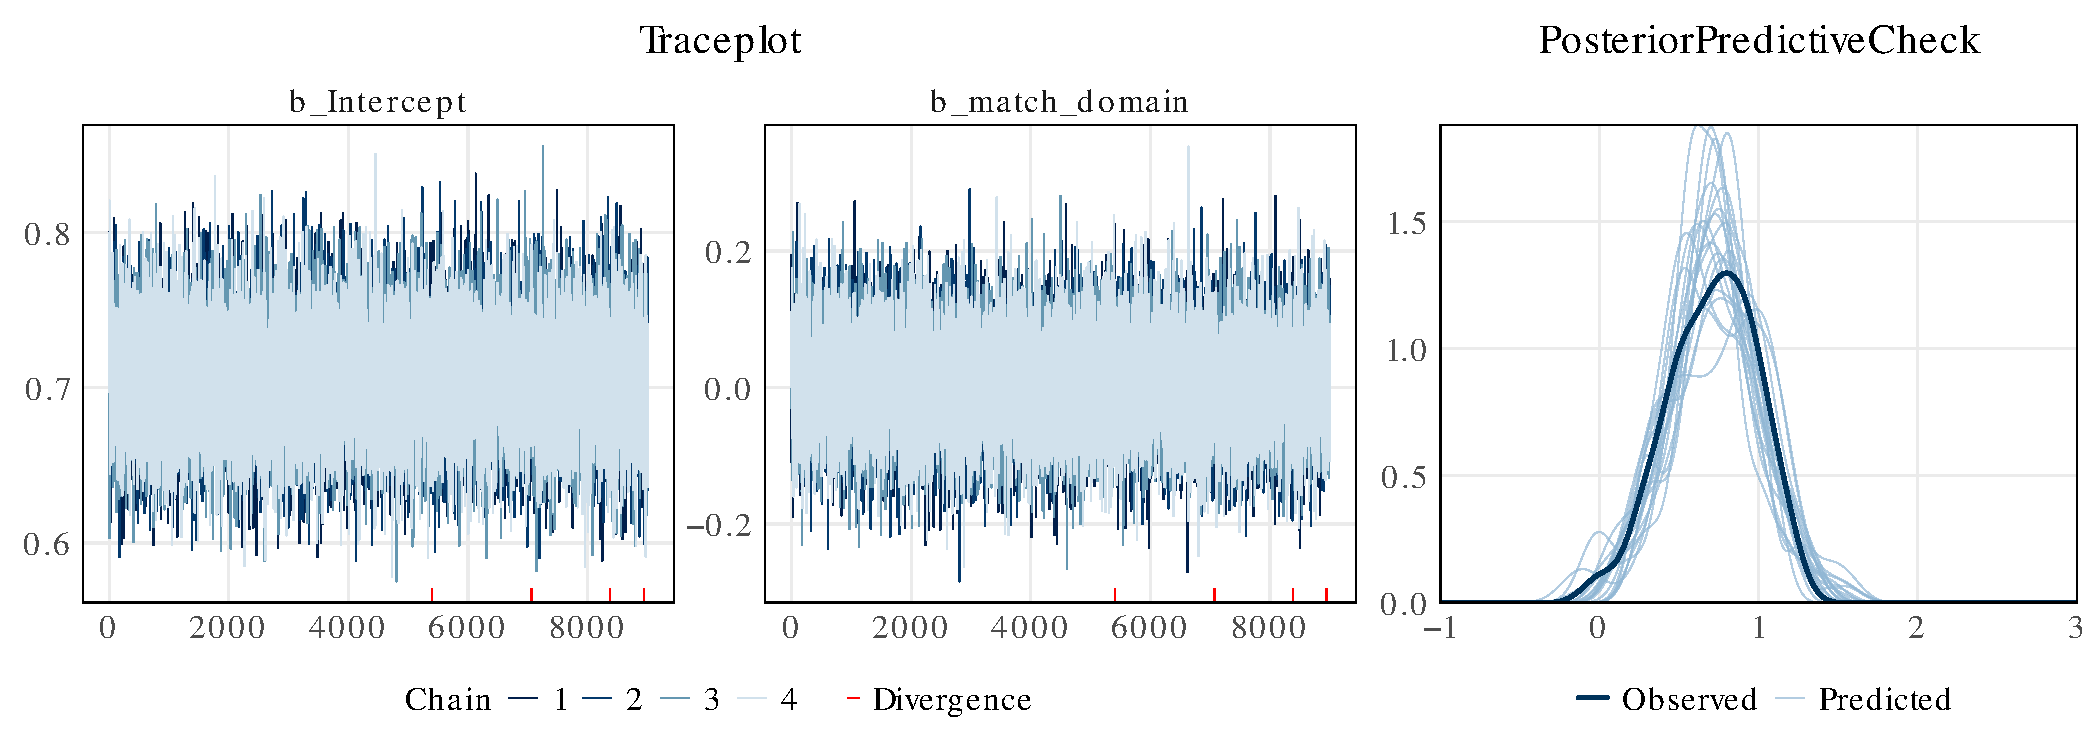
\includegraphics{supplement_files/figure-pdf/h1bM1CO2-1.pdf}

\subsubsection{kcal M0}\label{kcal-m0-1}

\begin{Shaded}
\begin{Highlighting}[]
\CommentTok{\# Load model }
\NormalTok{temp }\OtherTok{\textless{}{-}} \FunctionTok{brm}\NormalTok{(}\AttributeTok{file=}\StringTok{"../Results/fit\_H1b\_kcal\_M0.rds"}\NormalTok{)}

\CommentTok{\# Print Formular}
\NormalTok{temp}\SpecialCharTok{$}\NormalTok{formula}
\end{Highlighting}
\end{Shaded}

\begin{verbatim}
rank_z ~ 1 + (1 | ID) 
\end{verbatim}

\begin{Shaded}
\begin{Highlighting}[]
\CommentTok{\# Make model parameter table}
\FunctionTok{model\_parameters}\NormalTok{(temp, }\AttributeTok{centrality =} \StringTok{"mean"}\NormalTok{, }\AttributeTok{dispersion =} \ConstantTok{TRUE}\NormalTok{, }
                 \AttributeTok{ci\_method =} \StringTok{"hdi"}\NormalTok{, }\AttributeTok{effects =} \StringTok{"all"}\NormalTok{) }\SpecialCharTok{\%\textgreater{}\%} 
  \FunctionTok{kable}\NormalTok{(}\AttributeTok{digits=}\DecValTok{2}\NormalTok{) }\SpecialCharTok{\%\textgreater{}\%} \FunctionTok{kable\_paper}\NormalTok{()}
\end{Highlighting}
\end{Shaded}

\begin{longtable*}[t]{lllrrrrrrrrl}
\toprule
Parameter & Effects & Component & Mean & SD & CI & CI\_low & CI\_high & pd & Rhat & ESS & Group\\
\midrule
b\_Intercept & fixed & conditional & 0.91 & 0.04 & 0.95 & 0.83 & 0.99 & 1 & 1 & 17139.45 & \\
sd\_ID\_\_Intercept & random & conditional & 0.23 & 0.07 & 0.95 & 0.11 & 0.35 & 1 & 1 & 1609.94 & ID\\
sigma & fixed & sigma & 0.24 & 0.07 & 0.95 & 0.11 & 0.35 & 1 & 1 & 1339.11 & \\
\bottomrule
\end{longtable*}

\begin{Shaded}
\begin{Highlighting}[]
\CommentTok{\# Make trace and pp{-}check plot}
\FunctionTok{brms\_plot}\NormalTok{(temp,}\AttributeTok{lim=}\FunctionTok{c}\NormalTok{(}\SpecialCharTok{{-}}\DecValTok{1}\NormalTok{,}\DecValTok{3}\NormalTok{))}
\end{Highlighting}
\end{Shaded}

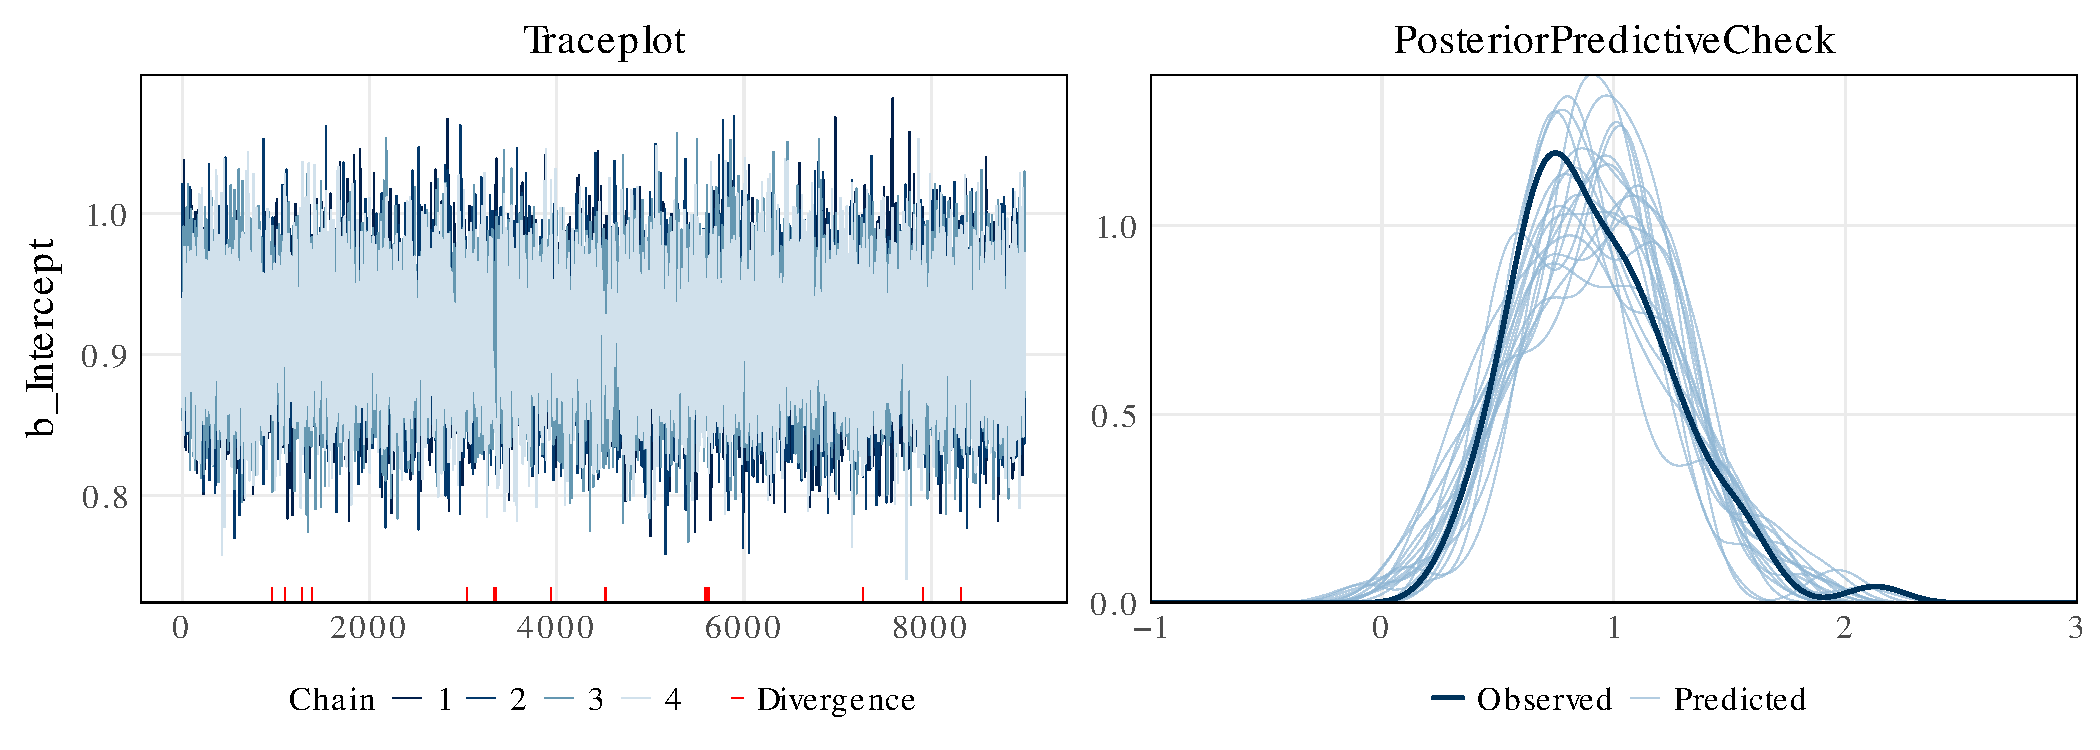
\includegraphics{supplement_files/figure-pdf/h1bM0kcal-1.pdf}

\subsubsection{kcal M1}\label{kcal-m1-1}

\begin{Shaded}
\begin{Highlighting}[]
\CommentTok{\# Load model }
\NormalTok{temp }\OtherTok{\textless{}{-}} \FunctionTok{brm}\NormalTok{(}\AttributeTok{file=}\StringTok{"../Results/fit\_H1b\_kcal\_M1.rds"}\NormalTok{)}

\CommentTok{\# Print Formular}
\NormalTok{temp}\SpecialCharTok{$}\NormalTok{formula}
\end{Highlighting}
\end{Shaded}

\begin{verbatim}
rank_z ~ match_domain + (1 | ID) 
\end{verbatim}

\begin{Shaded}
\begin{Highlighting}[]
\CommentTok{\# Make model parameter table}
\FunctionTok{model\_parameters}\NormalTok{(temp, }\AttributeTok{centrality =} \StringTok{"mean"}\NormalTok{, }\AttributeTok{dispersion =} \ConstantTok{TRUE}\NormalTok{, }
                 \AttributeTok{ci\_method =} \StringTok{"hdi"}\NormalTok{, }\AttributeTok{effects =} \StringTok{"all"}\NormalTok{) }\SpecialCharTok{\%\textgreater{}\%} 
  \FunctionTok{kable}\NormalTok{(}\AttributeTok{digits=}\DecValTok{2}\NormalTok{) }\SpecialCharTok{\%\textgreater{}\%} \FunctionTok{kable\_paper}\NormalTok{()}
\end{Highlighting}
\end{Shaded}

\begin{longtable*}[t]{lllrrrrrrrrl}
\toprule
Parameter & Effects & Component & Mean & SD & CI & CI\_low & CI\_high & pd & Rhat & ESS & Group\\
\midrule
b\_Intercept & fixed & conditional & 0.91 & 0.04 & 0.95 & 0.83 & 0.99 & 1.00 & 1 & 17275.08 & \\
b\_match\_domain & fixed & conditional & 0.11 & 0.08 & 0.95 & -0.05 & 0.26 & 0.92 & 1 & 15868.24 & \\
sd\_ID\_\_Intercept & random & conditional & 0.23 & 0.07 & 0.95 & 0.11 & 0.35 & 1.00 & 1 & 1336.84 & ID\\
sigma & fixed & sigma & 0.23 & 0.07 & 0.95 & 0.10 & 0.34 & 1.00 & 1 & 1003.81 & \\
\bottomrule
\end{longtable*}

\begin{Shaded}
\begin{Highlighting}[]
\CommentTok{\# Make trace and pp{-}check plot}
\FunctionTok{brms\_plot}\NormalTok{(temp,}\AttributeTok{lim=}\FunctionTok{c}\NormalTok{(}\SpecialCharTok{{-}}\DecValTok{1}\NormalTok{,}\DecValTok{3}\NormalTok{))  }\SpecialCharTok{+} \FunctionTok{plot\_layout}\NormalTok{(}\AttributeTok{widths =} \FunctionTok{c}\NormalTok{(}\DecValTok{2}\NormalTok{, }\DecValTok{1}\NormalTok{))}
\end{Highlighting}
\end{Shaded}

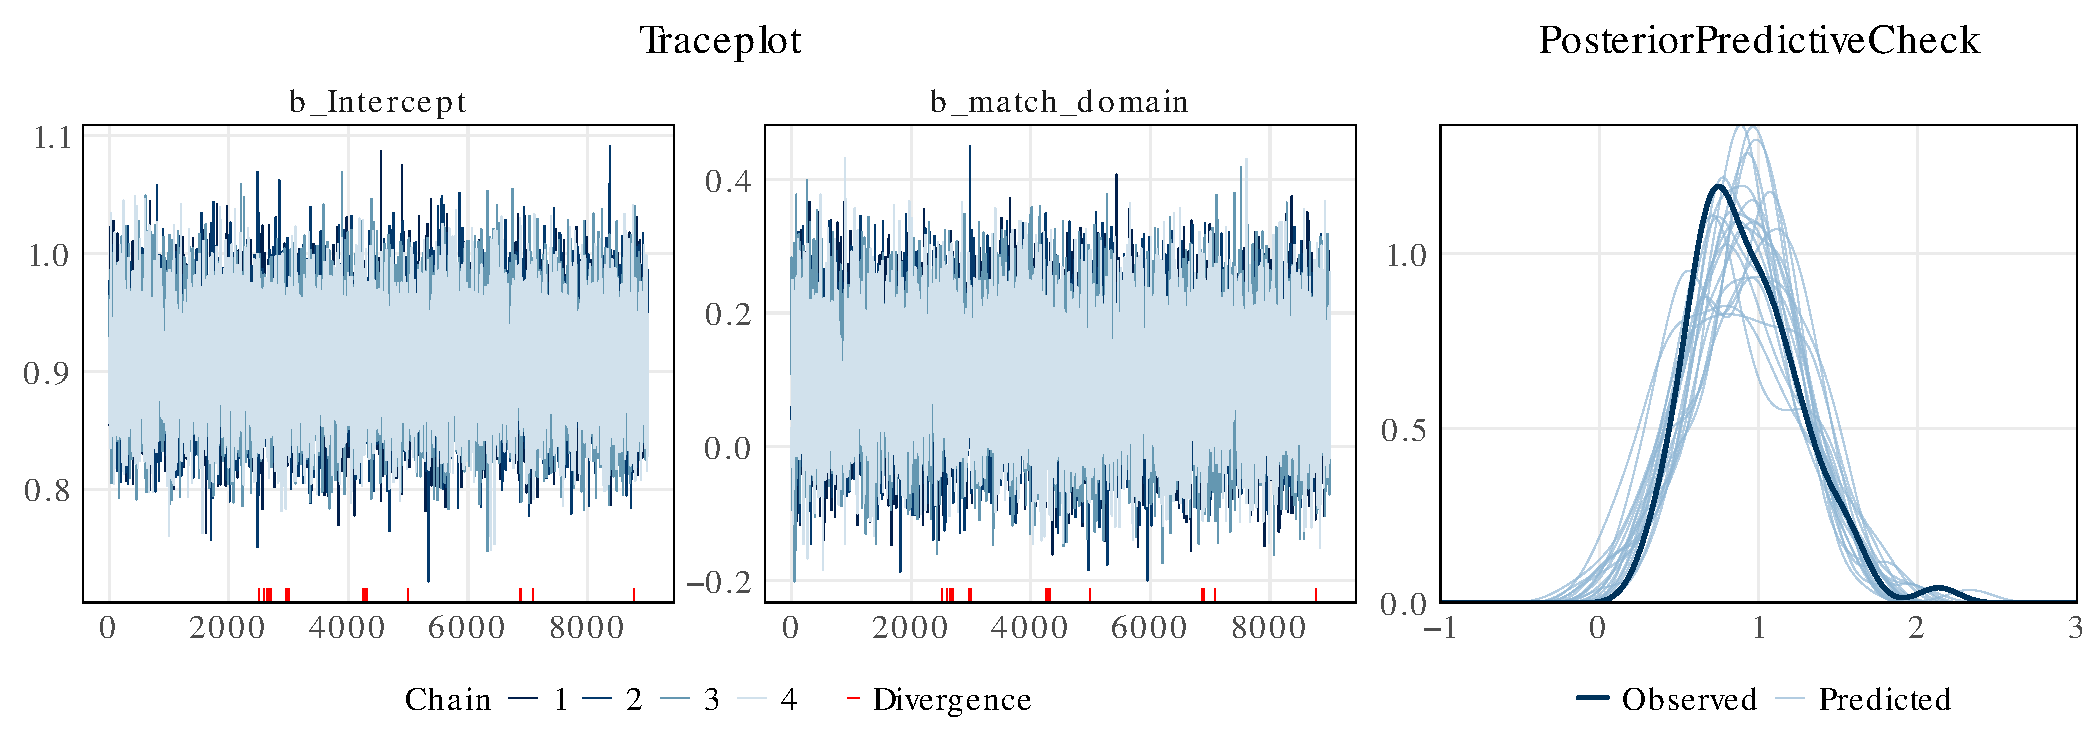
\includegraphics{supplement_files/figure-pdf/h1bM1kcal-1.pdf}

\subsection{Hypothesis 2a (OME)}\label{hypothesis-2a-ome}

\subsubsection{\texorpdfstring{CO\textsubscript{2}
M0}{CO2 M0}}\label{co2-m0-2}

\begin{Shaded}
\begin{Highlighting}[]
\CommentTok{\# Load model }
\NormalTok{temp }\OtherTok{\textless{}{-}} \FunctionTok{brm}\NormalTok{(}\AttributeTok{file=}\StringTok{"../Results/fit\_H2a\_CO2\_M0.rds"}\NormalTok{)}

\CommentTok{\# Print Formular}
\NormalTok{temp}\SpecialCharTok{$}\NormalTok{formula}
\end{Highlighting}
\end{Shaded}

\begin{verbatim}
OME_corr ~ 1 + (item_type | ID) + (1 | ID_item) 
\end{verbatim}

\begin{Shaded}
\begin{Highlighting}[]
\CommentTok{\# Make model parameter table}
\FunctionTok{model\_parameters}\NormalTok{(temp, }\AttributeTok{centrality =} \StringTok{"mean"}\NormalTok{, }\AttributeTok{dispersion =} \ConstantTok{TRUE}\NormalTok{, }
                 \AttributeTok{ci\_method =} \StringTok{"hdi"}\NormalTok{, }\AttributeTok{effects =} \StringTok{"all"}\NormalTok{) }\SpecialCharTok{\%\textgreater{}\%} 
  \FunctionTok{kable}\NormalTok{(}\AttributeTok{digits=}\DecValTok{2}\NormalTok{) }\SpecialCharTok{\%\textgreater{}\%} \FunctionTok{kable\_paper}\NormalTok{()}
\end{Highlighting}
\end{Shaded}

\begin{longtable*}[t]{lllrrrrrrrrl}
\toprule
Parameter & Effects & Component & Mean & SD & CI & CI\_low & CI\_high & pd & Rhat & ESS & Group\\
\midrule
b\_Intercept & fixed & conditional & -1.13 & 0.10 & 0.95 & -1.33 & -0.93 & 1.00 & 1 & 4031.52 & \\
sd\_ID\_\_Intercept & random & conditional & 0.47 & 0.06 & 0.95 & 0.36 & 0.60 & 1.00 & 1 & 6006.34 & ID\\
sd\_ID\_\_item\_type & random & conditional & 0.15 & 0.04 & 0.95 & 0.07 & 0.24 & 1.00 & 1 & 21140.26 & ID\\
sd\_ID\_item\_\_Intercept & random & conditional & 0.43 & 0.05 & 0.95 & 0.34 & 0.52 & 1.00 & 1 & 8220.85 & ID\_item\\
cor\_ID\_\_Intercept\_\_item\_type & random & conditional & -0.14 & 0.33 & 0.95 & -0.78 & 0.49 & 0.67 & 1 & 25947.13 & ID\\
\addlinespace
sigma & fixed & sigma & 0.99 & 0.02 & 0.95 & 0.96 & 1.02 & 1.00 & 1 & 38053.42 & \\
\bottomrule
\end{longtable*}

\begin{Shaded}
\begin{Highlighting}[]
\CommentTok{\# Make trace and pp{-}check plot}
\FunctionTok{brms\_plot}\NormalTok{(temp)}
\end{Highlighting}
\end{Shaded}

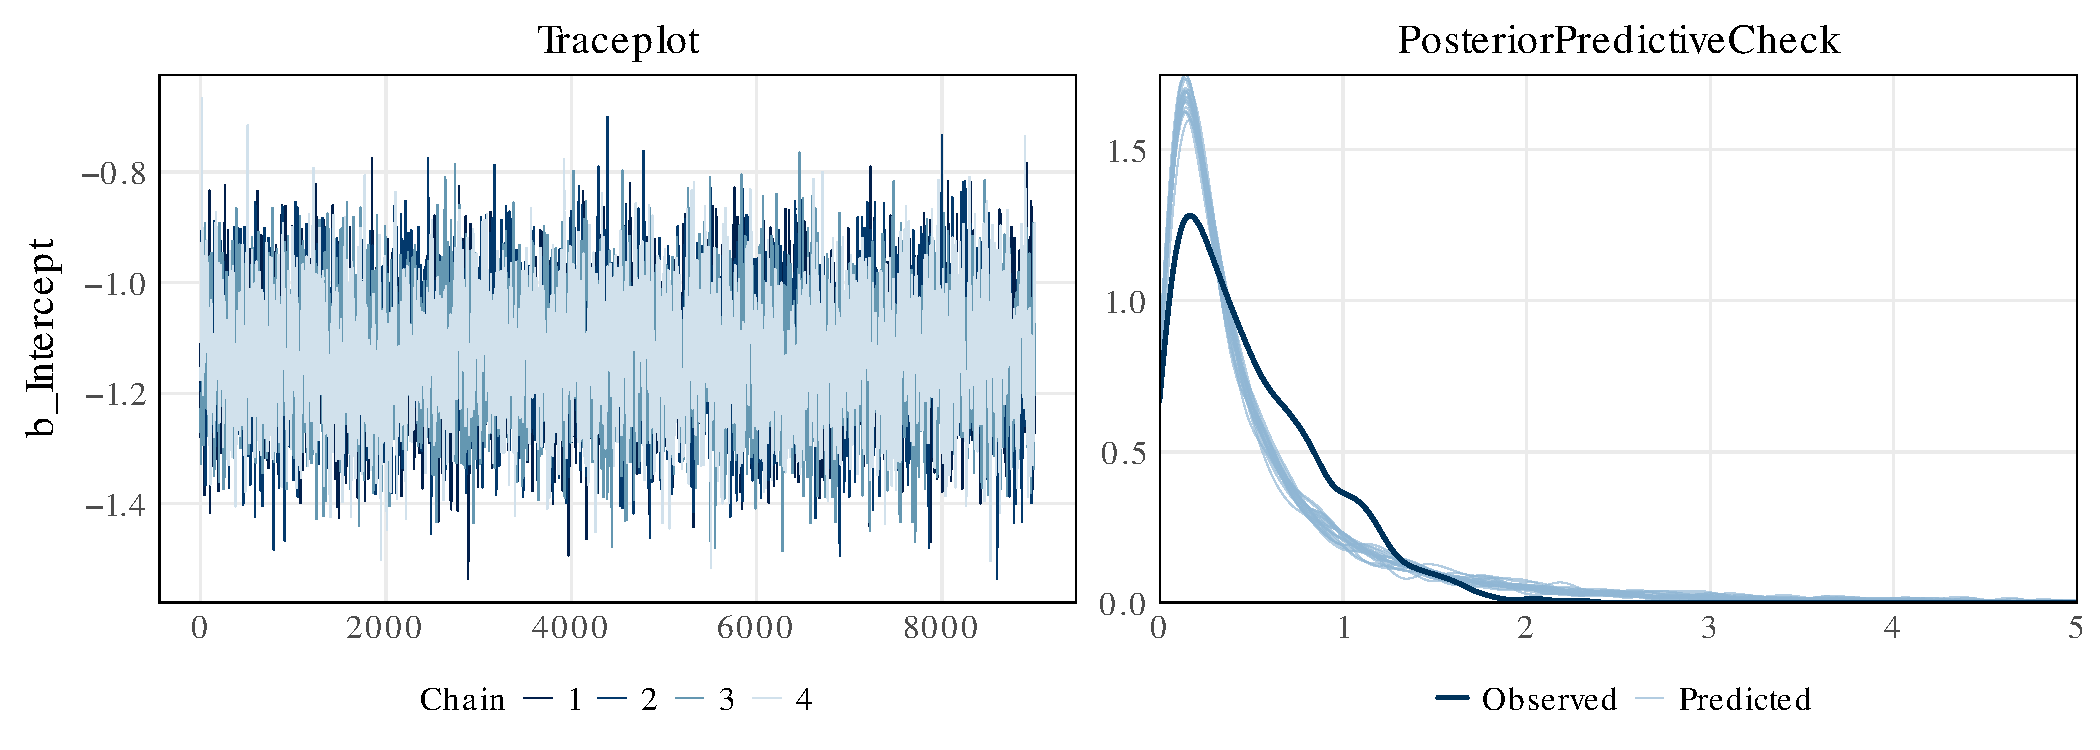
\includegraphics{supplement_files/figure-pdf/h2aM0CO2-1.pdf}

\subsubsection{\texorpdfstring{CO\textsubscript{2}
M1}{CO2 M1}}\label{co2-m1-2}

\begin{Shaded}
\begin{Highlighting}[]
\CommentTok{\# Load model }
\NormalTok{temp }\OtherTok{\textless{}{-}} \FunctionTok{brm}\NormalTok{(}\AttributeTok{file=}\StringTok{"../Results/fit\_H2a\_CO2\_M1.rds"}\NormalTok{)}

\CommentTok{\# Print Formular}
\NormalTok{temp}\SpecialCharTok{$}\NormalTok{formula}
\end{Highlighting}
\end{Shaded}

\begin{verbatim}
OME_corr ~ item_type + (item_type | ID) + (1 | ID_item) 
\end{verbatim}

\begin{Shaded}
\begin{Highlighting}[]
\CommentTok{\# Make model parameter table}
\FunctionTok{model\_parameters}\NormalTok{(temp, }\AttributeTok{centrality =} \StringTok{"mean"}\NormalTok{, }\AttributeTok{dispersion =} \ConstantTok{TRUE}\NormalTok{, }
                 \AttributeTok{ci\_method =} \StringTok{"hdi"}\NormalTok{, }\AttributeTok{effects =} \StringTok{"all"}\NormalTok{) }\SpecialCharTok{\%\textgreater{}\%} 
  \FunctionTok{kable}\NormalTok{(}\AttributeTok{digits=}\DecValTok{2}\NormalTok{) }\SpecialCharTok{\%\textgreater{}\%} \FunctionTok{kable\_paper}\NormalTok{()}
\end{Highlighting}
\end{Shaded}

\begin{longtable*}[t]{lllrrrrrrrrl}
\toprule
Parameter & Effects & Component & Mean & SD & CI & CI\_low & CI\_high & pd & Rhat & ESS & Group\\
\midrule
b\_Intercept & fixed & conditional & -1.14 & 0.10 & 0.95 & -1.34 & -0.93 & 1.00 & 1 & 4731.34 & \\
b\_item\_type & fixed & conditional & 0.04 & 0.12 & 0.95 & -0.19 & 0.27 & 0.65 & 1 & 9418.35 & \\
sd\_ID\_\_Intercept & random & conditional & 0.47 & 0.06 & 0.95 & 0.36 & 0.60 & 1.00 & 1 & 6815.38 & ID\\
sd\_ID\_\_item\_type & random & conditional & 0.15 & 0.04 & 0.95 & 0.08 & 0.24 & 1.00 & 1 & 22435.24 & ID\\
sd\_ID\_item\_\_Intercept & random & conditional & 0.43 & 0.05 & 0.95 & 0.35 & 0.53 & 1.00 & 1 & 8932.71 & ID\_item\\
\addlinespace
cor\_ID\_\_Intercept\_\_item\_type & random & conditional & -0.14 & 0.33 & 0.95 & -0.78 & 0.49 & 0.67 & 1 & 30353.00 & ID\\
sigma & fixed & sigma & 0.99 & 0.02 & 0.95 & 0.96 & 1.02 & 1.00 & 1 & 37143.68 & \\
\bottomrule
\end{longtable*}

\begin{Shaded}
\begin{Highlighting}[]
\CommentTok{\# Make trace and pp{-}check plot}
\FunctionTok{brms\_plot}\NormalTok{(temp)  }\SpecialCharTok{+} \FunctionTok{plot\_layout}\NormalTok{(}\AttributeTok{widths =} \FunctionTok{c}\NormalTok{(}\DecValTok{2}\NormalTok{, }\DecValTok{1}\NormalTok{))}
\end{Highlighting}
\end{Shaded}

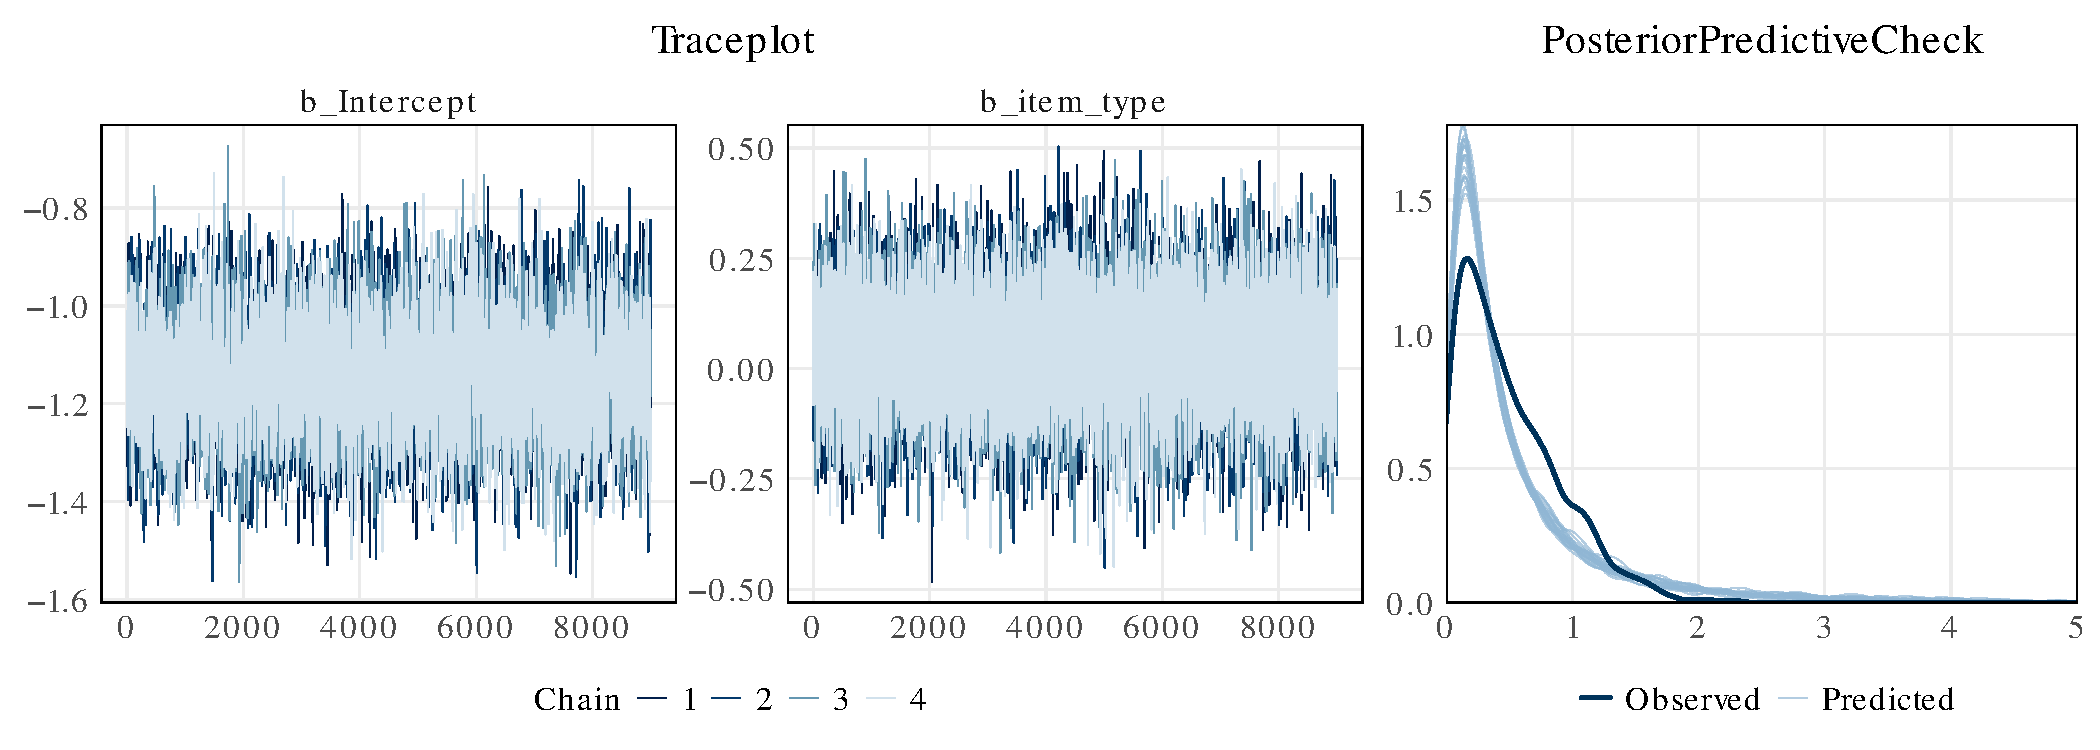
\includegraphics{supplement_files/figure-pdf/h2aM1CO2-1.pdf}

\subsubsection{kcal M0}\label{kcal-m0-2}

\begin{Shaded}
\begin{Highlighting}[]
\CommentTok{\# Load model }
\NormalTok{temp }\OtherTok{\textless{}{-}} \FunctionTok{brm}\NormalTok{(}\AttributeTok{file=}\StringTok{"../Results/fit\_H2a\_kcal\_M0.rds"}\NormalTok{)}

\CommentTok{\# Print Formular}
\NormalTok{temp}\SpecialCharTok{$}\NormalTok{formula}
\end{Highlighting}
\end{Shaded}

\begin{verbatim}
OME_corr ~ 1 + (item_type | ID) + (1 | ID_item) 
\end{verbatim}

\begin{Shaded}
\begin{Highlighting}[]
\CommentTok{\# Make model parameter table}
\FunctionTok{model\_parameters}\NormalTok{(temp, }\AttributeTok{centrality =} \StringTok{"mean"}\NormalTok{, }\AttributeTok{dispersion =} \ConstantTok{TRUE}\NormalTok{, }
                 \AttributeTok{ci\_method =} \StringTok{"hdi"}\NormalTok{, }\AttributeTok{effects =} \StringTok{"all"}\NormalTok{) }\SpecialCharTok{\%\textgreater{}\%} 
  \FunctionTok{kable}\NormalTok{(}\AttributeTok{digits=}\DecValTok{2}\NormalTok{) }\SpecialCharTok{\%\textgreater{}\%} \FunctionTok{kable\_paper}\NormalTok{()}
\end{Highlighting}
\end{Shaded}

\begin{longtable*}[t]{lllrrrrrrrrl}
\toprule
Parameter & Effects & Component & Mean & SD & CI & CI\_low & CI\_high & pd & Rhat & ESS & Group\\
\midrule
b\_Intercept & fixed & conditional & -2.01 & 0.09 & 0.95 & -2.19 & -1.83 & 1 & 1 & 4561.44 & \\
sd\_ID\_\_Intercept & random & conditional & 0.60 & 0.07 & 0.95 & 0.46 & 0.73 & 1 & 1 & 7841.60 & ID\\
sd\_ID\_\_item\_type & random & conditional & 0.78 & 0.10 & 0.95 & 0.58 & 0.97 & 1 & 1 & 10922.07 & ID\\
sd\_ID\_item\_\_Intercept & random & conditional & 0.35 & 0.04 & 0.95 & 0.27 & 0.44 & 1 & 1 & 12363.74 & ID\_item\\
cor\_ID\_\_Intercept\_\_item\_type & random & conditional & -0.69 & 0.10 & 0.95 & -0.86 & -0.50 & 1 & 1 & 10593.49 & ID\\
\addlinespace
sigma & fixed & sigma & 1.21 & 0.02 & 0.95 & 1.18 & 1.25 & 1 & 1 & 42025.21 & \\
\bottomrule
\end{longtable*}

\begin{Shaded}
\begin{Highlighting}[]
\CommentTok{\# Make trace and pp{-}check plot}
\FunctionTok{brms\_plot}\NormalTok{(temp)}
\end{Highlighting}
\end{Shaded}

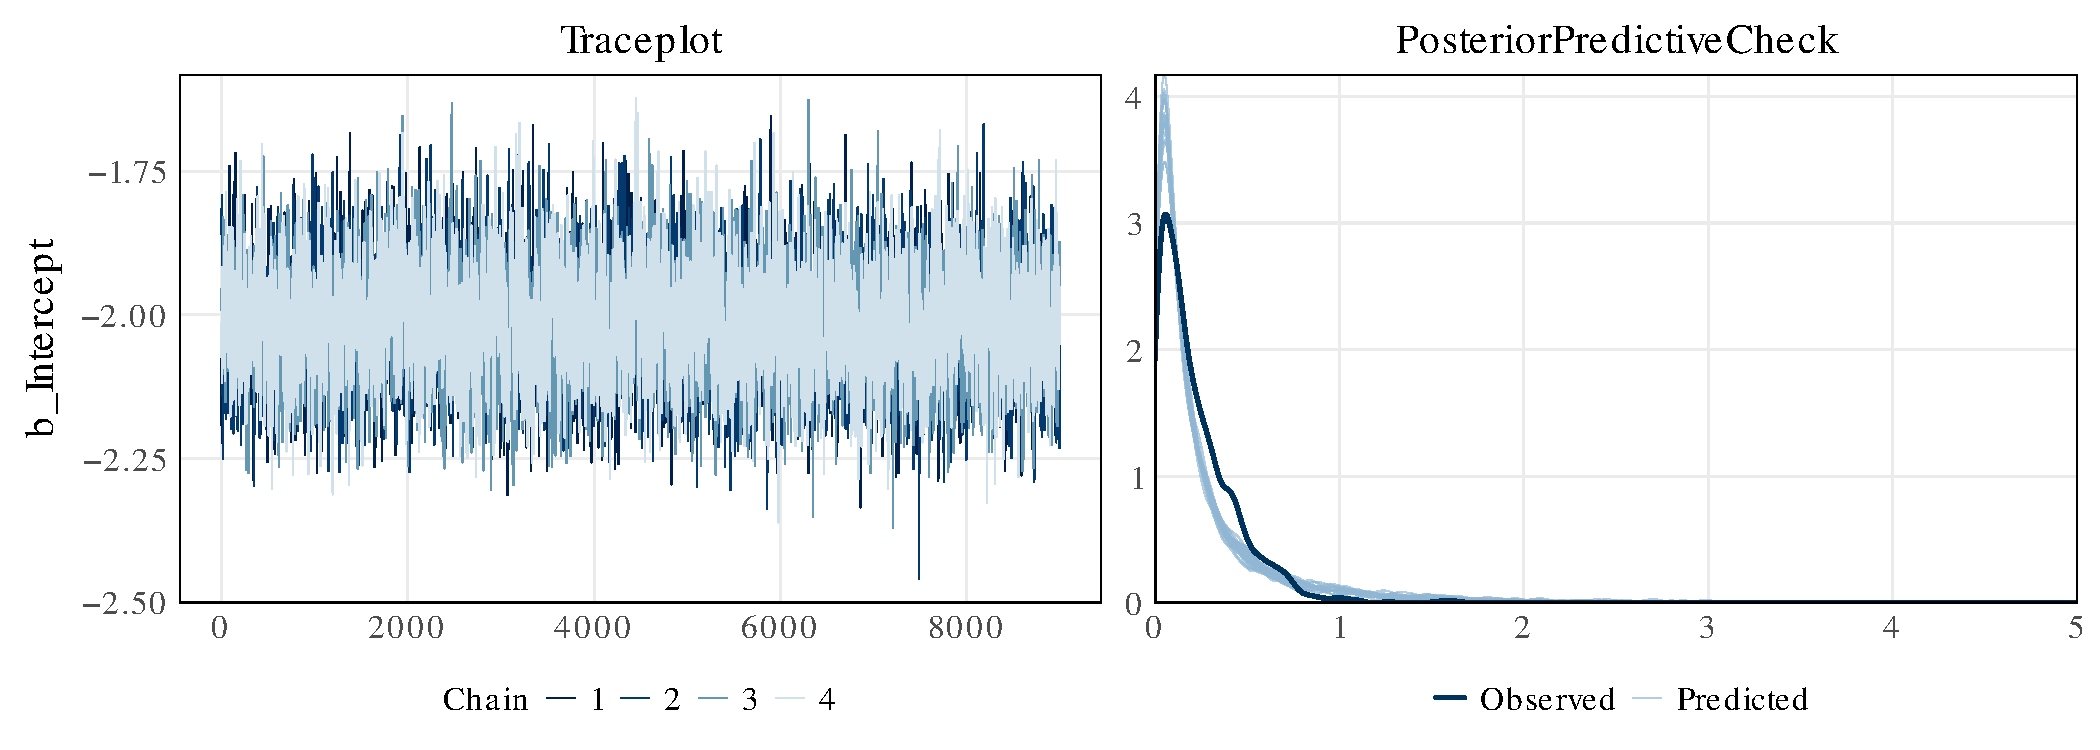
\includegraphics{supplement_files/figure-pdf/h2aM0kcal-1.pdf}

\subsubsection{kcal M1}\label{kcal-m1-2}

\begin{Shaded}
\begin{Highlighting}[]
\CommentTok{\# Load model }
\NormalTok{temp }\OtherTok{\textless{}{-}} \FunctionTok{brm}\NormalTok{(}\AttributeTok{file=}\StringTok{"../Results/fit\_H2a\_kcal\_M1.rds"}\NormalTok{)}

\CommentTok{\# Print Formular}
\NormalTok{temp}\SpecialCharTok{$}\NormalTok{formula}
\end{Highlighting}
\end{Shaded}

\begin{verbatim}
OME_corr ~ item_type + (item_type | ID) + (1 | ID_item) 
\end{verbatim}

\begin{Shaded}
\begin{Highlighting}[]
\CommentTok{\# Make model parameter table}
\FunctionTok{model\_parameters}\NormalTok{(temp, }\AttributeTok{centrality =} \StringTok{"mean"}\NormalTok{, }\AttributeTok{dispersion =} \ConstantTok{TRUE}\NormalTok{, }
                 \AttributeTok{ci\_method =} \StringTok{"hdi"}\NormalTok{, }\AttributeTok{effects =} \StringTok{"all"}\NormalTok{) }\SpecialCharTok{\%\textgreater{}\%} 
  \FunctionTok{kable}\NormalTok{(}\AttributeTok{digits=}\DecValTok{2}\NormalTok{) }\SpecialCharTok{\%\textgreater{}\%} \FunctionTok{kable\_paper}\NormalTok{()}
\end{Highlighting}
\end{Shaded}

\begin{longtable*}[t]{lllrrrrrrrrl}
\toprule
Parameter & Effects & Component & Mean & SD & CI & CI\_low & CI\_high & pd & Rhat & ESS & Group\\
\midrule
b\_Intercept & fixed & conditional & -2.09 & 0.10 & 0.95 & -2.29 & -1.88 & 1.00 & 1 & 5533.01 & \\
b\_item\_type & fixed & conditional & 0.20 & 0.14 & 0.95 & -0.07 & 0.46 & 0.93 & 1 & 10816.30 & \\
sd\_ID\_\_Intercept & random & conditional & 0.59 & 0.07 & 0.95 & 0.46 & 0.73 & 1.00 & 1 & 8270.44 & ID\\
sd\_ID\_\_item\_type & random & conditional & 0.77 & 0.10 & 0.95 & 0.58 & 0.97 & 1.00 & 1 & 12159.10 & ID\\
sd\_ID\_item\_\_Intercept & random & conditional & 0.35 & 0.04 & 0.95 & 0.27 & 0.43 & 1.00 & 1 & 12931.42 & ID\_item\\
\addlinespace
cor\_ID\_\_Intercept\_\_item\_type & random & conditional & -0.68 & 0.10 & 0.95 & -0.86 & -0.49 & 1.00 & 1 & 12831.05 & ID\\
sigma & fixed & sigma & 1.21 & 0.02 & 0.95 & 1.18 & 1.25 & 1.00 & 1 & 48437.01 & \\
\bottomrule
\end{longtable*}

\begin{Shaded}
\begin{Highlighting}[]
\CommentTok{\# Make trace and pp{-}check plot}
\FunctionTok{brms\_plot}\NormalTok{(temp)  }\SpecialCharTok{+} \FunctionTok{plot\_layout}\NormalTok{(}\AttributeTok{widths =} \FunctionTok{c}\NormalTok{(}\DecValTok{2}\NormalTok{, }\DecValTok{1}\NormalTok{))}
\end{Highlighting}
\end{Shaded}

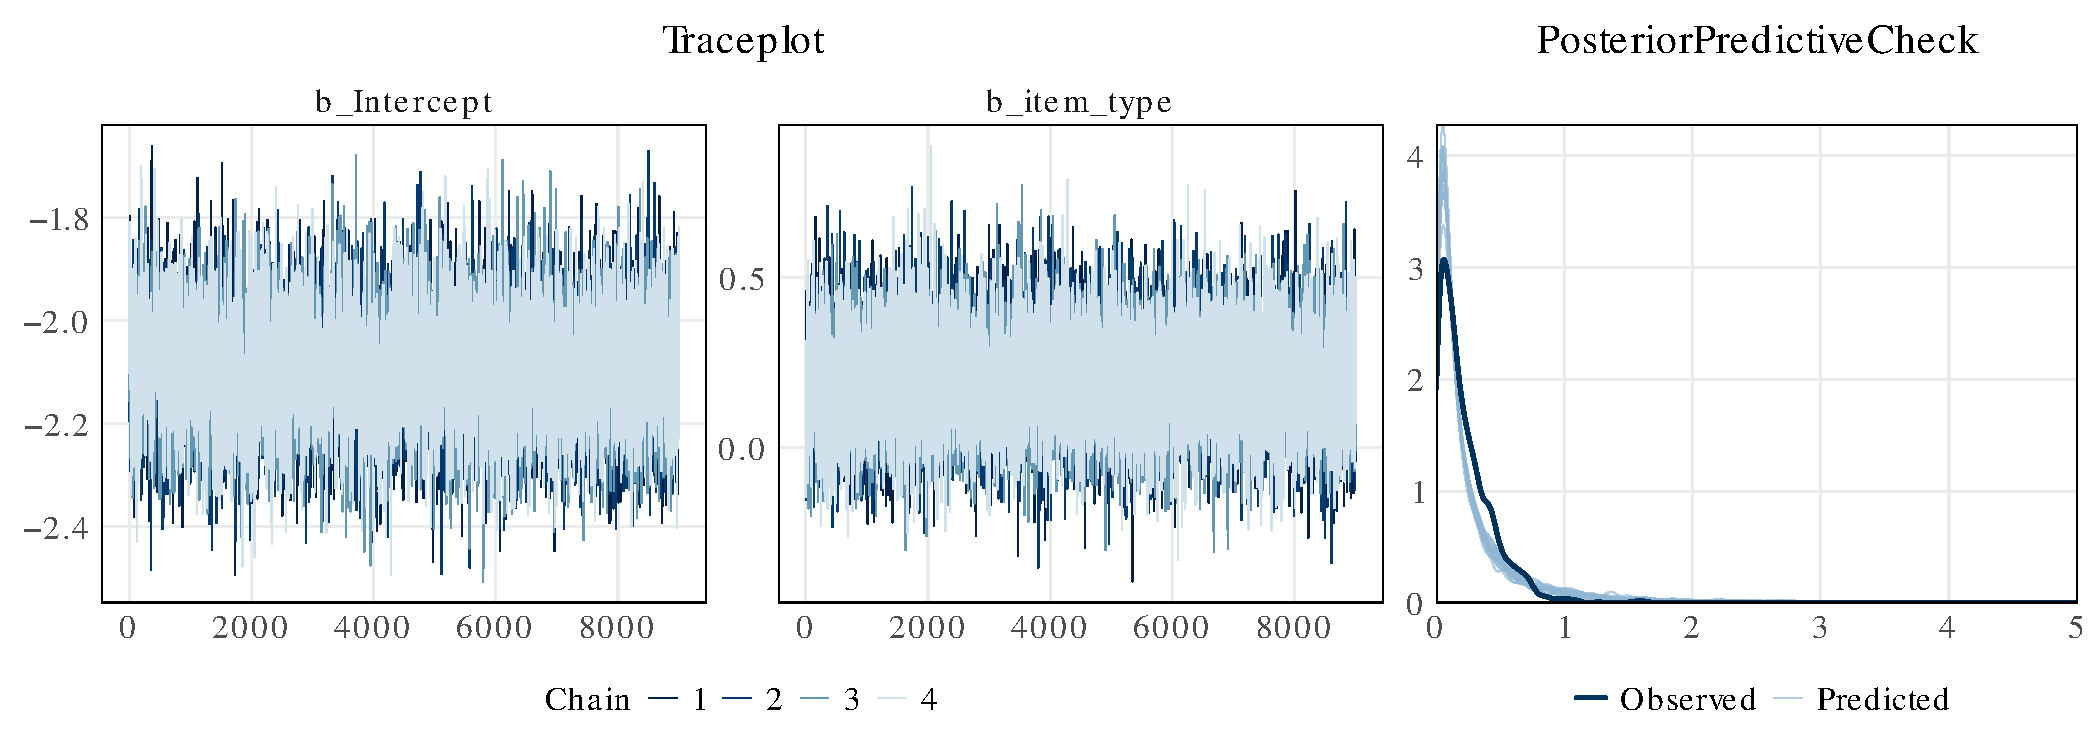
\includegraphics{supplement_files/figure-pdf/h2aM1kcal-1.pdf}

\subsection{\texorpdfstring{Hypothesis 2b
(\(\rho\))}{Hypothesis 2b (\textbackslash rho)}}\label{hypothesis-2b-rho}

\subsubsection{\texorpdfstring{CO\textsubscript{2}
M0}{CO2 M0}}\label{co2-m0-3}

\begin{Shaded}
\begin{Highlighting}[]
\CommentTok{\# Load model }
\NormalTok{temp }\OtherTok{\textless{}{-}} \FunctionTok{brm}\NormalTok{(}\AttributeTok{file=}\StringTok{"../Results/fit\_H2b\_CO2\_M0.rds"}\NormalTok{)}

\CommentTok{\# Print Formular}
\NormalTok{temp}\SpecialCharTok{$}\NormalTok{formula}
\end{Highlighting}
\end{Shaded}

\begin{verbatim}
rank_z ~ 1 + (item_type | ID) 
\end{verbatim}

\begin{Shaded}
\begin{Highlighting}[]
\CommentTok{\# Make model parameter table}
\FunctionTok{model\_parameters}\NormalTok{(temp, }\AttributeTok{centrality =} \StringTok{"mean"}\NormalTok{, }\AttributeTok{dispersion =} \ConstantTok{TRUE}\NormalTok{, }
                 \AttributeTok{ci\_method =} \StringTok{"hdi"}\NormalTok{, }\AttributeTok{effects =} \StringTok{"all"}\NormalTok{) }\SpecialCharTok{\%\textgreater{}\%} 
  \FunctionTok{kable}\NormalTok{(}\AttributeTok{digits=}\DecValTok{2}\NormalTok{) }\SpecialCharTok{\%\textgreater{}\%} \FunctionTok{kable\_paper}\NormalTok{()}
\end{Highlighting}
\end{Shaded}

\begin{longtable*}[t]{lllrrrrrrrrl}
\toprule
Parameter & Effects & Component & Mean & SD & CI & CI\_low & CI\_high & pd & Rhat & ESS & Group\\
\midrule
b\_Intercept & fixed & conditional & 0.71 & 0.05 & 0.95 & 0.62 & 0.81 & 1.00 & 1 & 12636.07 & \\
sd\_ID\_\_Intercept & random & conditional & 0.26 & 0.04 & 0.95 & 0.18 & 0.34 & 1.00 & 1 & 8553.85 & ID\\
sd\_ID\_\_item\_type & random & conditional & 0.18 & 0.05 & 0.95 & 0.09 & 0.27 & 1.00 & 1 & 8509.64 & ID\\
cor\_ID\_\_Intercept\_\_item\_type & random & conditional & -0.48 & 0.30 & 0.95 & -1.00 & 0.03 & 0.94 & 1 & 19603.18 & ID\\
sigma & fixed & sigma & 0.17 & 0.03 & 0.95 & 0.10 & 0.24 & 1.00 & 1 & 4446.90 & \\
\bottomrule
\end{longtable*}

\begin{Shaded}
\begin{Highlighting}[]
\CommentTok{\# Make trace and pp{-}check plot}
\FunctionTok{brms\_plot}\NormalTok{(temp,}\AttributeTok{lim=}\FunctionTok{c}\NormalTok{(}\SpecialCharTok{{-}}\DecValTok{1}\NormalTok{,}\DecValTok{3}\NormalTok{))}
\end{Highlighting}
\end{Shaded}

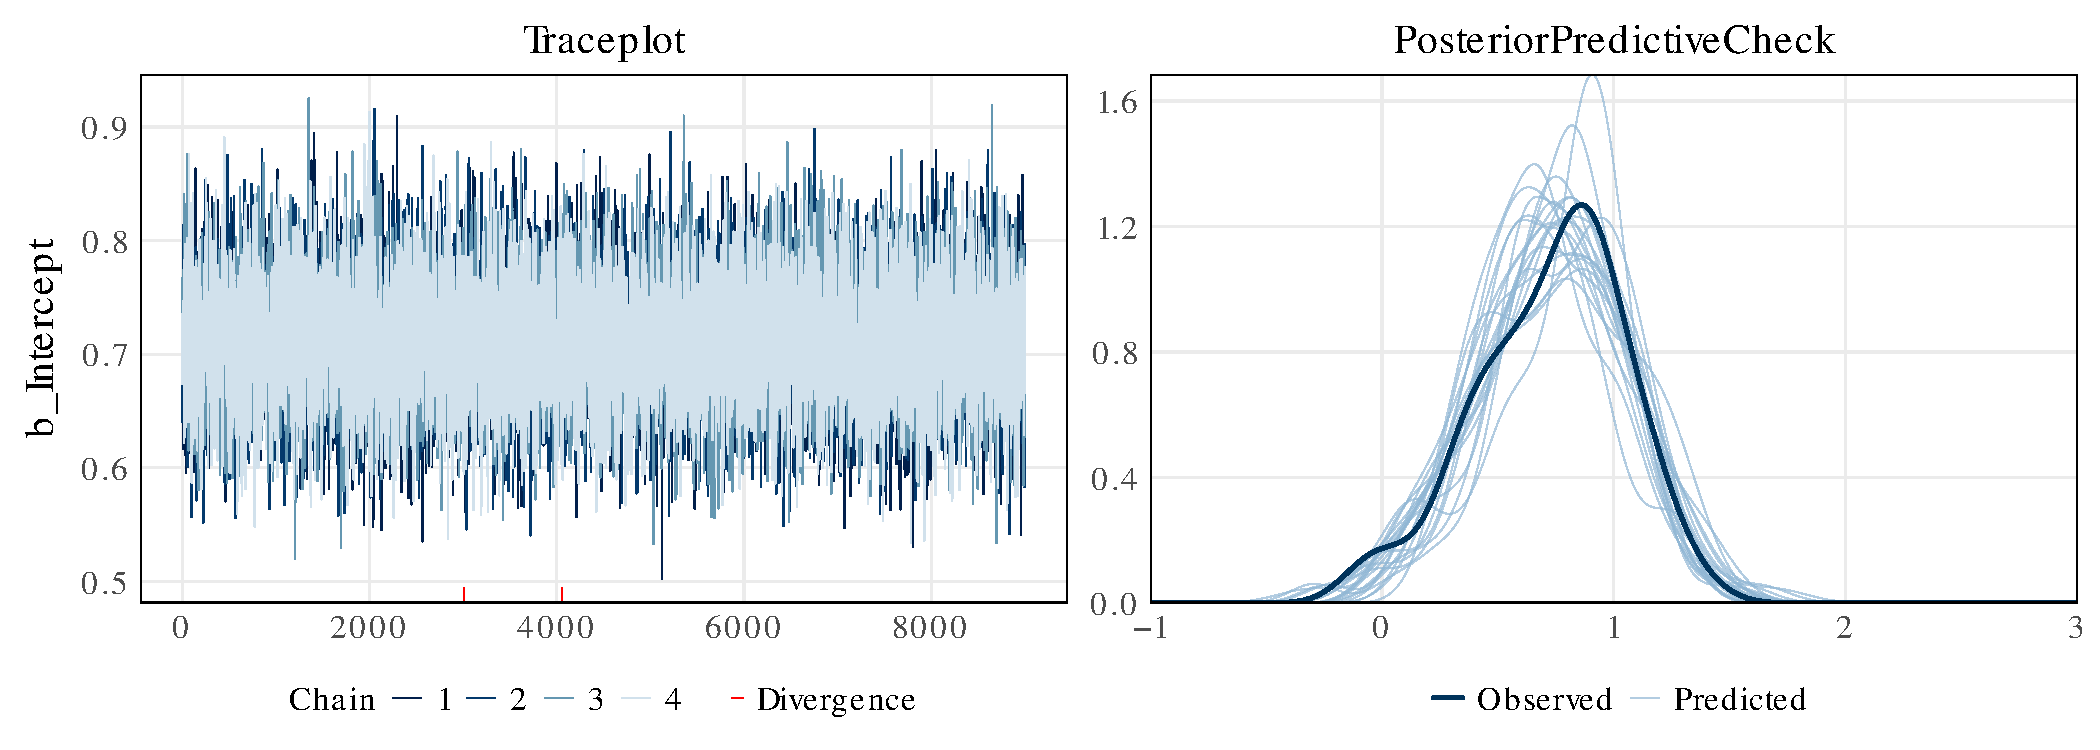
\includegraphics{supplement_files/figure-pdf/h2bM0CO2-1.pdf}

\subsubsection{\texorpdfstring{CO\textsubscript{2}
M1}{CO2 M1}}\label{co2-m1-3}

\begin{Shaded}
\begin{Highlighting}[]
\CommentTok{\# Load model }
\NormalTok{temp }\OtherTok{\textless{}{-}} \FunctionTok{brm}\NormalTok{(}\AttributeTok{file=}\StringTok{"../Results/fit\_H2b\_CO2\_M1.rds"}\NormalTok{)}

\CommentTok{\# Print Formular}
\NormalTok{temp}\SpecialCharTok{$}\NormalTok{formula}
\end{Highlighting}
\end{Shaded}

\begin{verbatim}
rank_z ~ item_type + (item_type | ID) 
\end{verbatim}

\begin{Shaded}
\begin{Highlighting}[]
\CommentTok{\# Make model parameter table}
\FunctionTok{model\_parameters}\NormalTok{(temp, }\AttributeTok{centrality =} \StringTok{"mean"}\NormalTok{, }\AttributeTok{dispersion =} \ConstantTok{TRUE}\NormalTok{, }
                 \AttributeTok{ci\_method =} \StringTok{"hdi"}\NormalTok{, }\AttributeTok{effects =} \StringTok{"all"}\NormalTok{) }\SpecialCharTok{\%\textgreater{}\%} 
  \FunctionTok{kable}\NormalTok{(}\AttributeTok{digits=}\DecValTok{2}\NormalTok{) }\SpecialCharTok{\%\textgreater{}\%} \FunctionTok{kable\_paper}\NormalTok{()}
\end{Highlighting}
\end{Shaded}

\begin{longtable*}[t]{lllrrrrrrrrl}
\toprule
Parameter & Effects & Component & Mean & SD & CI & CI\_low & CI\_high & pd & Rhat & ESS & Group\\
\midrule
b\_Intercept & fixed & conditional & 0.72 & 0.05 & 0.95 & 0.62 & 0.82 & 1.00 & 1 & 10424.50 & \\
b\_item\_type & fixed & conditional & -0.03 & 0.06 & 0.95 & -0.13 & 0.08 & 0.69 & 1 & 27912.14 & \\
sd\_ID\_\_Intercept & random & conditional & 0.26 & 0.04 & 0.95 & 0.18 & 0.34 & 1.00 & 1 & 7414.75 & ID\\
sd\_ID\_\_item\_type & random & conditional & 0.18 & 0.05 & 0.95 & 0.09 & 0.28 & 1.00 & 1 & 6578.21 & ID\\
cor\_ID\_\_Intercept\_\_item\_type & random & conditional & -0.48 & 0.30 & 0.95 & -1.00 & 0.04 & 0.94 & 1 & 18649.40 & ID\\
\addlinespace
sigma & fixed & sigma & 0.17 & 0.03 & 0.95 & 0.10 & 0.24 & 1.00 & 1 & 4057.54 & \\
\bottomrule
\end{longtable*}

\begin{Shaded}
\begin{Highlighting}[]
\CommentTok{\# Make trace and pp{-}check plot}
\FunctionTok{brms\_plot}\NormalTok{(temp,}\AttributeTok{lim=}\FunctionTok{c}\NormalTok{(}\SpecialCharTok{{-}}\DecValTok{1}\NormalTok{,}\DecValTok{3}\NormalTok{))  }\SpecialCharTok{+} \FunctionTok{plot\_layout}\NormalTok{(}\AttributeTok{widths =} \FunctionTok{c}\NormalTok{(}\DecValTok{2}\NormalTok{, }\DecValTok{1}\NormalTok{))}
\end{Highlighting}
\end{Shaded}

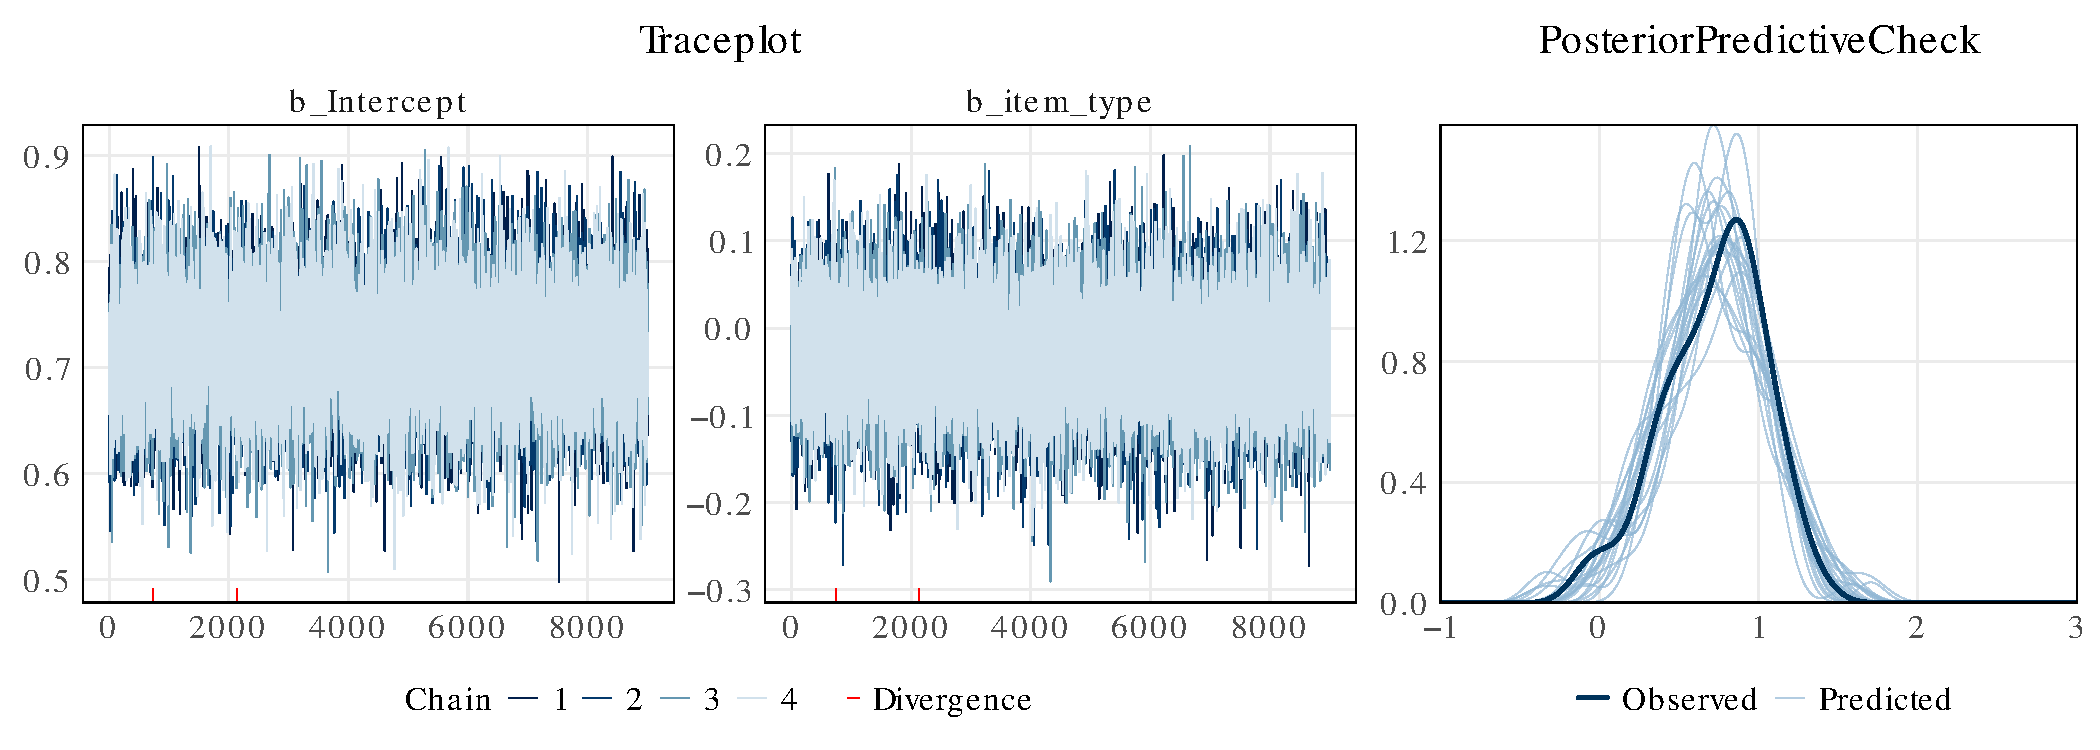
\includegraphics{supplement_files/figure-pdf/h2bM1CO2-1.pdf}

\subsubsection{kcal M0}\label{kcal-m0-3}

\begin{Shaded}
\begin{Highlighting}[]
\CommentTok{\# Load model }
\NormalTok{temp }\OtherTok{\textless{}{-}} \FunctionTok{brm}\NormalTok{(}\AttributeTok{file=}\StringTok{"../Results/fit\_H2b\_kcal\_M0.rds"}\NormalTok{)}

\CommentTok{\# Print Formular}
\NormalTok{temp}\SpecialCharTok{$}\NormalTok{formula}
\end{Highlighting}
\end{Shaded}

\begin{verbatim}
rank_z ~ 1 + (item_type | ID) 
\end{verbatim}

\begin{Shaded}
\begin{Highlighting}[]
\CommentTok{\# Make model parameter table}
\FunctionTok{model\_parameters}\NormalTok{(temp, }\AttributeTok{centrality =} \StringTok{"mean"}\NormalTok{, }\AttributeTok{dispersion =} \ConstantTok{TRUE}\NormalTok{, }
                 \AttributeTok{ci\_method =} \StringTok{"hdi"}\NormalTok{, }\AttributeTok{effects =} \StringTok{"all"}\NormalTok{) }\SpecialCharTok{\%\textgreater{}\%} 
  \FunctionTok{kable}\NormalTok{(}\AttributeTok{digits=}\DecValTok{2}\NormalTok{) }\SpecialCharTok{\%\textgreater{}\%} \FunctionTok{kable\_paper}\NormalTok{()}
\end{Highlighting}
\end{Shaded}

\begin{longtable*}[t]{lllrrrrrrrrl}
\toprule
Parameter & Effects & Component & Mean & SD & CI & CI\_low & CI\_high & pd & Rhat & ESS & Group\\
\midrule
b\_Intercept & fixed & conditional & 1.01 & 0.06 & 0.95 & 0.89 & 1.12 & 1.00 & 1 & 9734.39 & \\
sd\_ID\_\_Intercept & random & conditional & 0.30 & 0.05 & 0.95 & 0.21 & 0.40 & 1.00 & 1 & 6318.78 & ID\\
sd\_ID\_\_item\_type & random & conditional & 0.20 & 0.07 & 0.95 & 0.08 & 0.32 & 1.00 & 1 & 4021.79 & ID\\
cor\_ID\_\_Intercept\_\_item\_type & random & conditional & -0.34 & 0.34 & 0.95 & -1.00 & 0.25 & 0.85 & 1 & 15988.18 & ID\\
sigma & fixed & sigma & 0.22 & 0.04 & 0.95 & 0.13 & 0.31 & 1.00 & 1 & 2530.04 & \\
\bottomrule
\end{longtable*}

\begin{Shaded}
\begin{Highlighting}[]
\CommentTok{\# Make trace and pp{-}check plot}
\FunctionTok{brms\_plot}\NormalTok{(temp,}\AttributeTok{lim=}\FunctionTok{c}\NormalTok{(}\SpecialCharTok{{-}}\DecValTok{1}\NormalTok{,}\DecValTok{3}\NormalTok{))}
\end{Highlighting}
\end{Shaded}

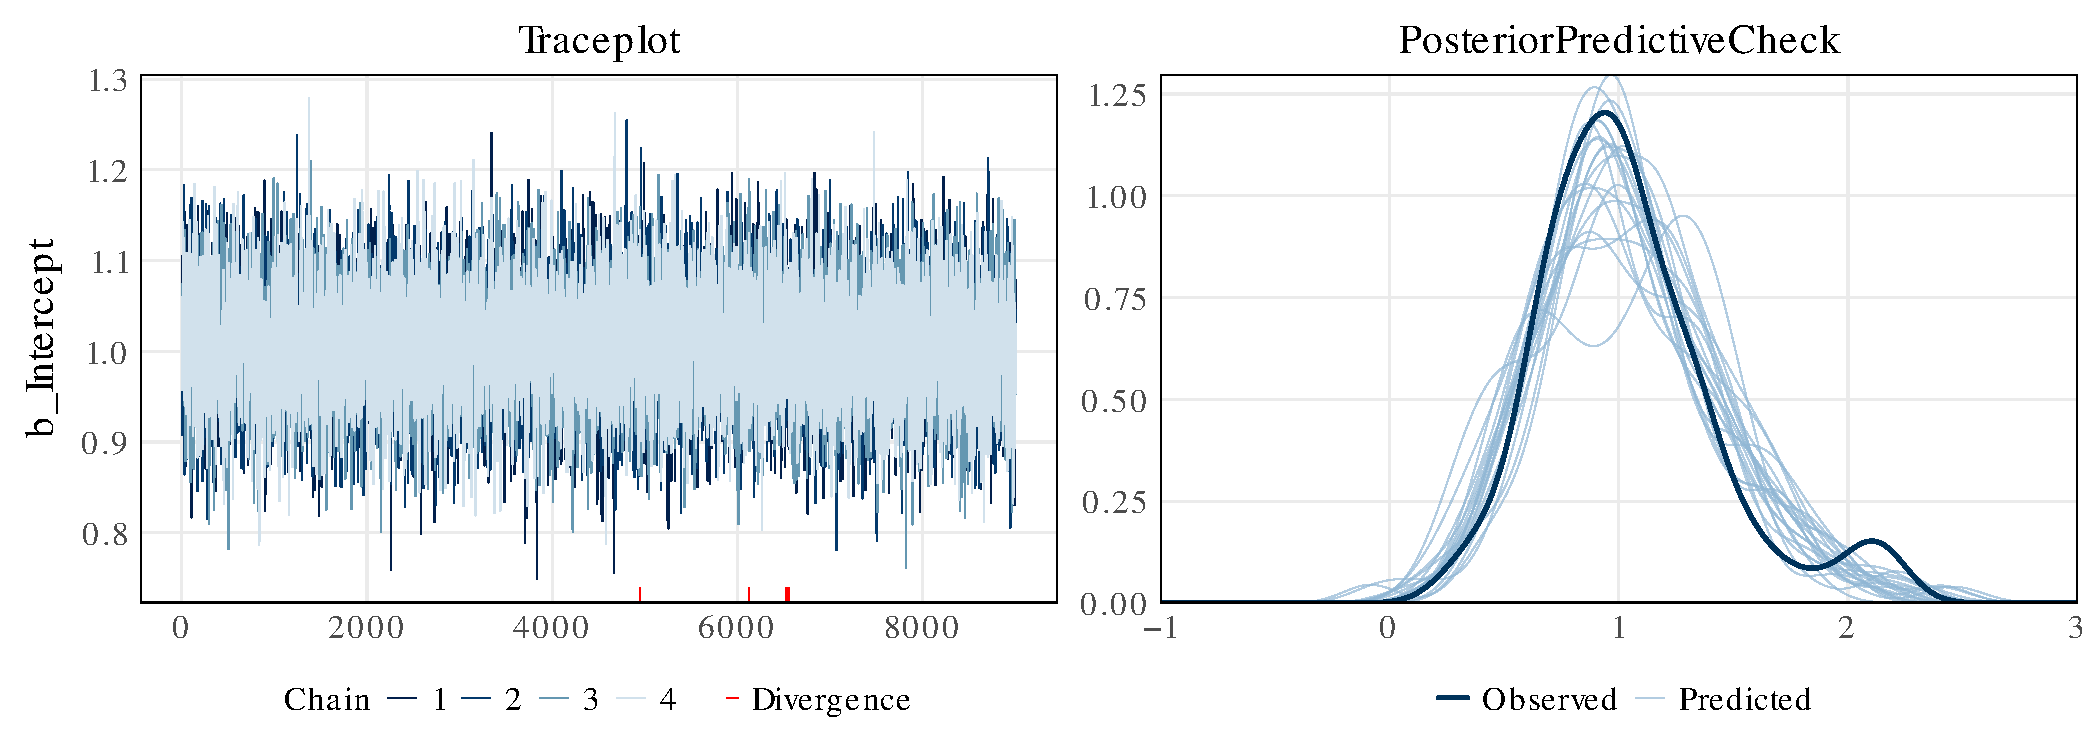
\includegraphics{supplement_files/figure-pdf/h2bM0kcal-1.pdf}

\subsubsection{kcal M1}\label{kcal-m1-3}

\begin{Shaded}
\begin{Highlighting}[]
\CommentTok{\# Load model }
\NormalTok{temp }\OtherTok{\textless{}{-}} \FunctionTok{brm}\NormalTok{(}\AttributeTok{file=}\StringTok{"../Results/fit\_H2b\_kcal\_M1.rds"}\NormalTok{)}

\CommentTok{\# Print Formular}
\NormalTok{temp}\SpecialCharTok{$}\NormalTok{formula}
\end{Highlighting}
\end{Shaded}

\begin{verbatim}
rank_z ~ item_type + (item_type | ID) 
\end{verbatim}

\begin{Shaded}
\begin{Highlighting}[]
\CommentTok{\# Make model parameter table}
\FunctionTok{model\_parameters}\NormalTok{(temp, }\AttributeTok{centrality =} \StringTok{"mean"}\NormalTok{, }\AttributeTok{dispersion =} \ConstantTok{TRUE}\NormalTok{, }
                 \AttributeTok{ci\_method =} \StringTok{"hdi"}\NormalTok{, }\AttributeTok{effects =} \StringTok{"all"}\NormalTok{) }\SpecialCharTok{\%\textgreater{}\%} 
  \FunctionTok{kable}\NormalTok{(}\AttributeTok{digits=}\DecValTok{2}\NormalTok{) }\SpecialCharTok{\%\textgreater{}\%} \FunctionTok{kable\_paper}\NormalTok{()}
\end{Highlighting}
\end{Shaded}

\begin{longtable*}[t]{lllrrrrrrrrl}
\toprule
Parameter & Effects & Component & Mean & SD & CI & CI\_low & CI\_high & pd & Rhat & ESS & Group\\
\midrule
b\_Intercept & fixed & conditional & 1.02 & 0.06 & 0.95 & 0.91 & 1.13 & 1.00 & 1 & 10035.23 & \\
b\_item\_type & fixed & conditional & -0.13 & 0.06 & 0.95 & -0.25 & -0.01 & 0.99 & 1 & 27882.90 & \\
sd\_ID\_\_Intercept & random & conditional & 0.30 & 0.05 & 0.95 & 0.21 & 0.40 & 1.00 & 1 & 6567.08 & ID\\
sd\_ID\_\_item\_type & random & conditional & 0.19 & 0.06 & 0.95 & 0.08 & 0.31 & 1.00 & 1 & 3844.00 & ID\\
cor\_ID\_\_Intercept\_\_item\_type & random & conditional & -0.32 & 0.34 & 0.95 & -1.00 & 0.26 & 0.83 & 1 & 19119.58 & ID\\
\addlinespace
sigma & fixed & sigma & 0.21 & 0.04 & 0.95 & 0.12 & 0.29 & 1.00 & 1 & 2707.32 & \\
\bottomrule
\end{longtable*}

\begin{Shaded}
\begin{Highlighting}[]
\CommentTok{\# Make trace and pp{-}check plot}
\FunctionTok{brms\_plot}\NormalTok{(temp,}\AttributeTok{lim=}\FunctionTok{c}\NormalTok{(}\SpecialCharTok{{-}}\DecValTok{1}\NormalTok{,}\DecValTok{3}\NormalTok{))  }\SpecialCharTok{+} \FunctionTok{plot\_layout}\NormalTok{(}\AttributeTok{widths =} \FunctionTok{c}\NormalTok{(}\DecValTok{2}\NormalTok{, }\DecValTok{1}\NormalTok{))}
\end{Highlighting}
\end{Shaded}

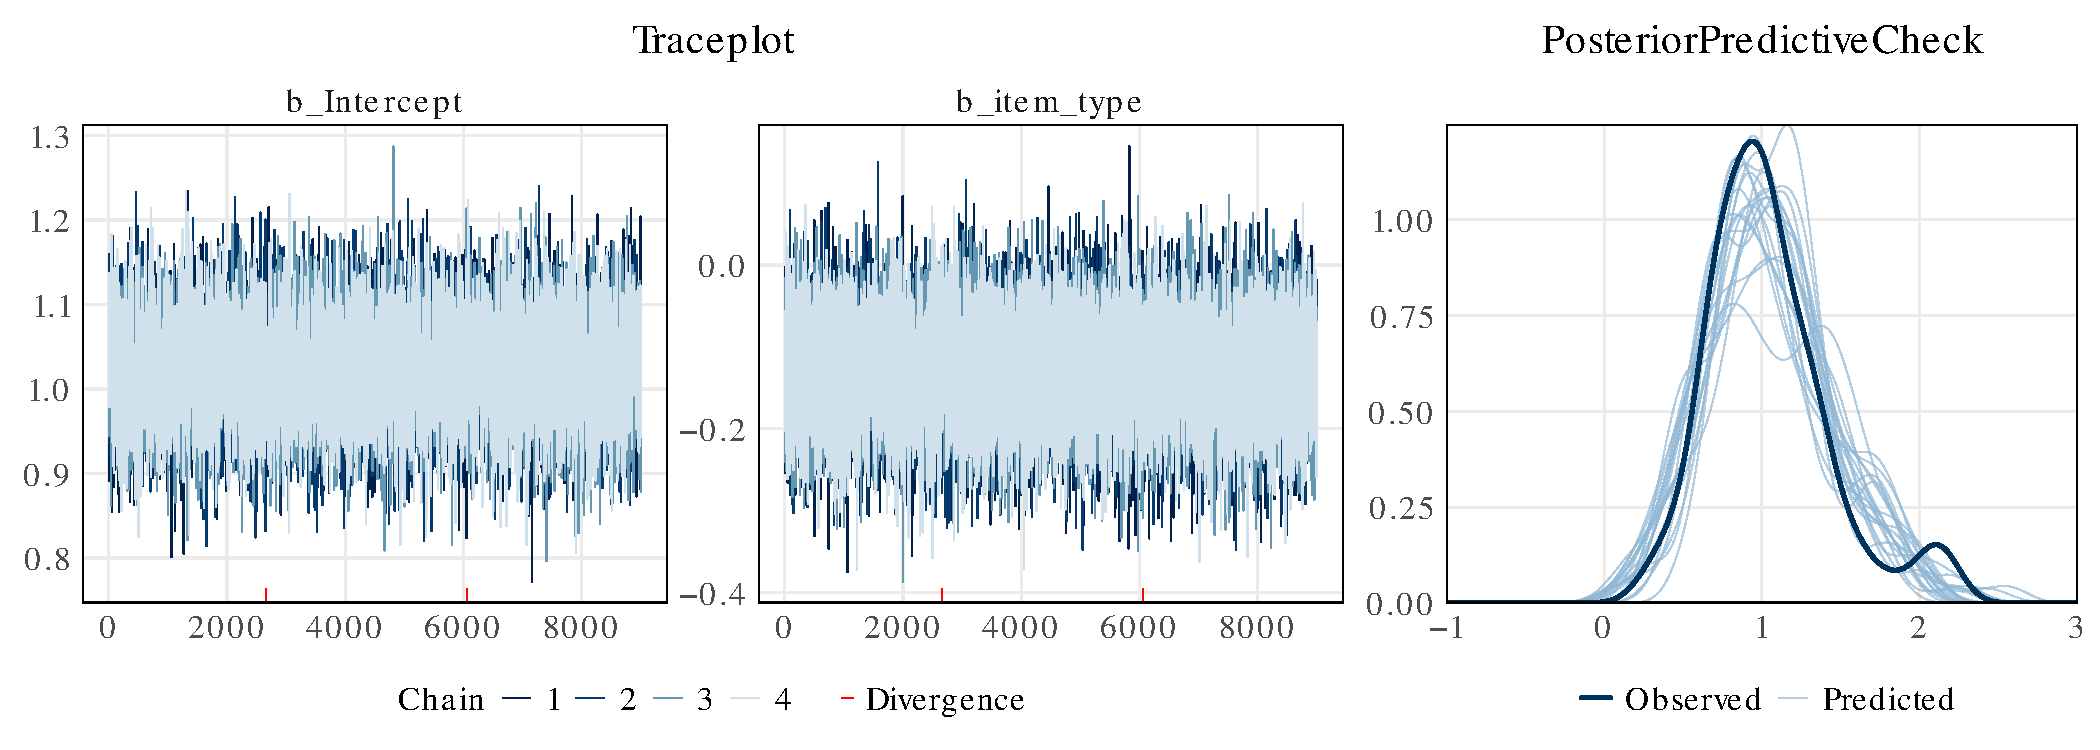
\includegraphics{supplement_files/figure-pdf/h2bM1kcal-1.pdf}

\subsection{Hypothesis 3a (OME)}\label{hypothesis-3a-ome}

\subsubsection{M0}\label{m0}

\begin{Shaded}
\begin{Highlighting}[]
\CommentTok{\# Load model }
\NormalTok{temp }\OtherTok{\textless{}{-}} \FunctionTok{brm}\NormalTok{(}\AttributeTok{file=}\StringTok{"../Results/fit\_H3a\_M0.rds"}\NormalTok{)}

\CommentTok{\# Print Formular}
\NormalTok{temp}\SpecialCharTok{$}\NormalTok{formula}
\end{Highlighting}
\end{Shaded}

\begin{verbatim}
OME_corr ~ match_domain + (1 | ID) + (est_criterion * match_domain | ID_item) 
\end{verbatim}

\begin{Shaded}
\begin{Highlighting}[]
\CommentTok{\# Make model parameter table}
\FunctionTok{model\_parameters}\NormalTok{(temp, }\AttributeTok{centrality =} \StringTok{"mean"}\NormalTok{, }\AttributeTok{dispersion =} \ConstantTok{TRUE}\NormalTok{, }
                 \AttributeTok{ci\_method =} \StringTok{"hdi"}\NormalTok{, }\AttributeTok{effects =} \StringTok{"all"}\NormalTok{) }\SpecialCharTok{\%\textgreater{}\%} 
  \FunctionTok{kable}\NormalTok{(}\AttributeTok{digits=}\DecValTok{2}\NormalTok{) }\SpecialCharTok{\%\textgreater{}\%} \FunctionTok{kable\_paper}\NormalTok{()}
\end{Highlighting}
\end{Shaded}

\begin{longtable*}[t]{lllrrrrrrrrl}
\toprule
Parameter & Effects & Component & Mean & SD & CI & CI\_low & CI\_high & pd & Rhat & ESS & Group\\
\midrule
b\_Intercept & fixed & conditional & -1.23 & 0.08 & 0.95 & -1.39 & -1.07 & 1.00 & 1 & 3452.18 & \\
b\_match\_domain & fixed & conditional & -0.49 & 0.13 & 0.95 & -0.75 & -0.24 & 1.00 & 1 & 3316.02 & \\
sd\_ID\_\_Intercept & random & conditional & 0.75 & 0.06 & 0.95 & 0.64 & 0.87 & 1.00 & 1 & 3134.21 & ID\\
sd\_ID\_item\_\_Intercept & random & conditional & 0.33 & 0.04 & 0.95 & 0.25 & 0.40 & 1.00 & 1 & 6601.40 & ID\_item\\
sd\_ID\_item\_\_est\_criterionKcal & random & conditional & 0.57 & 0.09 & 0.95 & 0.40 & 0.75 & 1.00 & 1 & 1856.29 & ID\_item\\
\addlinespace
sd\_ID\_item\_\_match\_domain & random & conditional & 0.16 & 0.03 & 0.95 & 0.09 & 0.22 & 1.00 & 1 & 30559.02 & ID\_item\\
sd\_ID\_item\_\_est\_criterionKcal:match\_domain & random & conditional & 0.17 & 0.05 & 0.95 & 0.08 & 0.26 & 1.00 & 1 & 24982.57 & ID\_item\\
cor\_ID\_item\_\_Intercept\_\_est\_criterionKcal & random & conditional & -0.60 & 0.11 & 0.95 & -0.80 & -0.38 & 1.00 & 1 & 3265.99 & ID\_item\\
cor\_ID\_item\_\_Intercept\_\_match\_domain & random & conditional & 0.69 & 0.17 & 0.95 & 0.35 & 0.96 & 1.00 & 1 & 28574.51 & ID\_item\\
cor\_ID\_item\_\_est\_criterionKcal\_\_match\_domain & random & conditional & -0.42 & 0.24 & 0.95 & -0.85 & 0.05 & 0.95 & 1 & 23990.17 & ID\_item\\
\addlinespace
cor\_ID\_item\_\_Intercept\_\_est\_criterionKcal:match\_domain & random & conditional & -0.45 & 0.26 & 0.95 & -0.90 & 0.07 & 0.94 & 1 & 22933.27 & ID\_item\\
cor\_ID\_item\_\_est\_criterionKcal\_\_est\_criterionKcal:match\_domain & random & conditional & 0.19 & 0.31 & 0.95 & -0.40 & 0.78 & 0.73 & 1 & 19336.61 & ID\_item\\
cor\_ID\_item\_\_match\_domain\_\_est\_criterionKcal:match\_domain & random & conditional & -0.57 & 0.25 & 0.95 & -0.96 & -0.09 & 0.97 & 1 & 25143.64 & ID\_item\\
sigma & fixed & sigma & 1.05 & 0.01 & 0.95 & 1.03 & 1.07 & 1.00 & 1 & 72737.31 & \\
\bottomrule
\end{longtable*}

\begin{Shaded}
\begin{Highlighting}[]
\CommentTok{\# Make trace and pp{-}check plot}
\FunctionTok{brms\_plot}\NormalTok{(temp) }\SpecialCharTok{+} \FunctionTok{plot\_layout}\NormalTok{(}\AttributeTok{widths =} \FunctionTok{c}\NormalTok{(}\DecValTok{2}\NormalTok{, }\DecValTok{1}\NormalTok{))}
\end{Highlighting}
\end{Shaded}

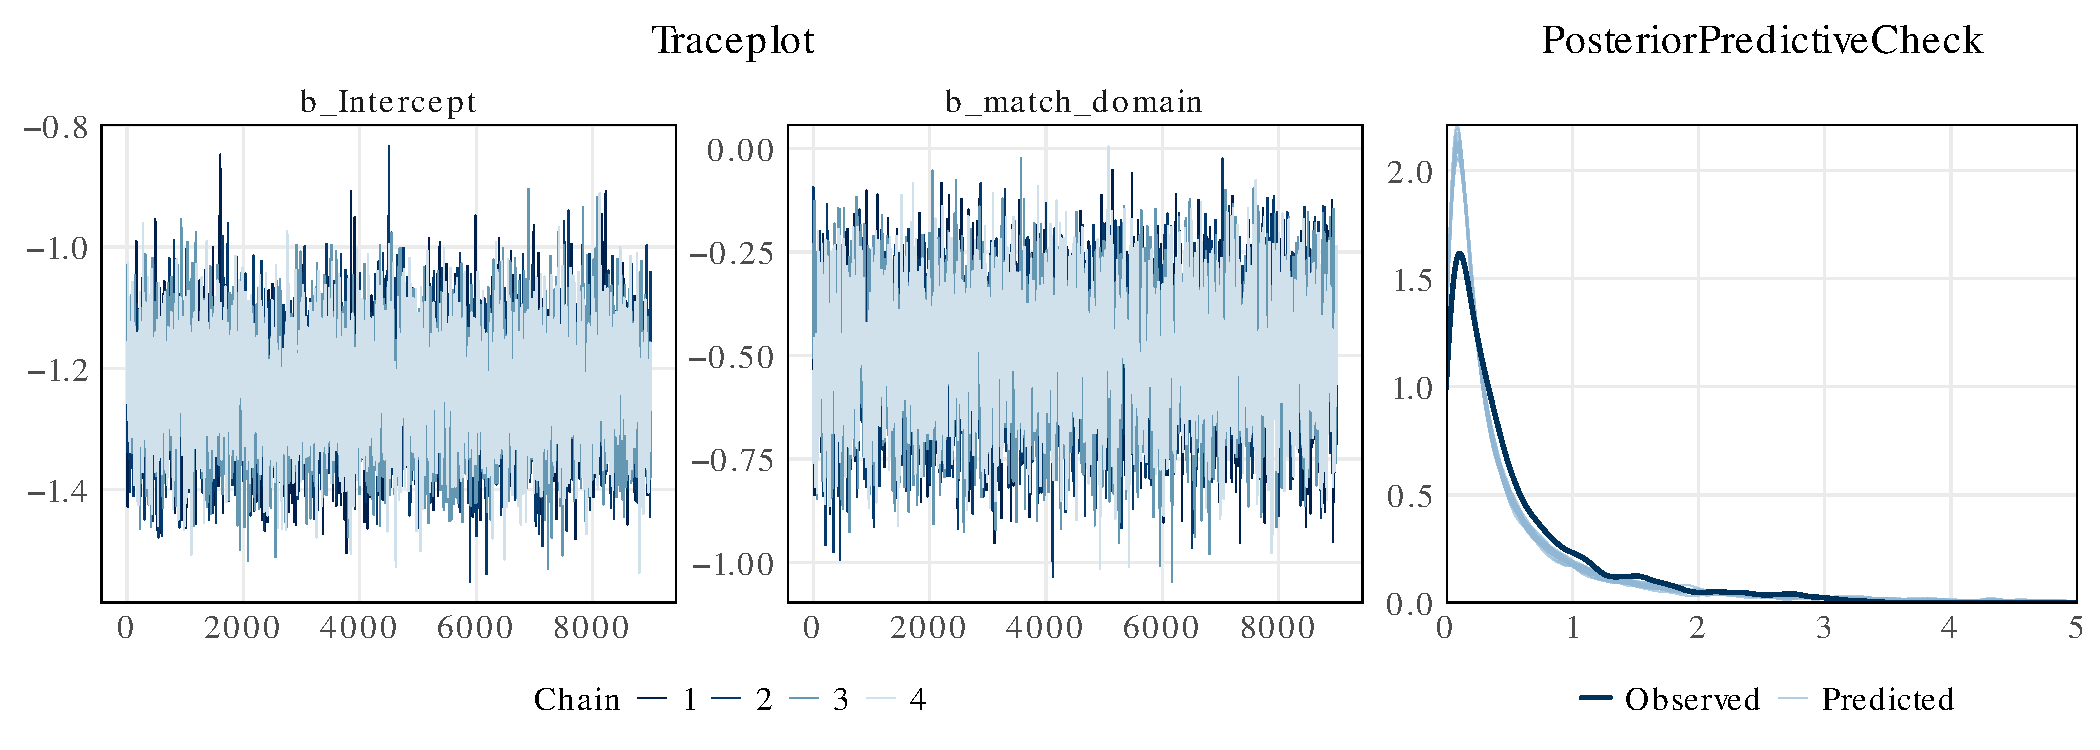
\includegraphics{supplement_files/figure-pdf/h3aM0-1.pdf}

\subsubsection{M1}\label{m1}

\begin{Shaded}
\begin{Highlighting}[]
\CommentTok{\# Load model }
\NormalTok{temp }\OtherTok{\textless{}{-}} \FunctionTok{brm}\NormalTok{(}\AttributeTok{file=}\StringTok{"../Results/fit\_H3a\_M1.rds"}\NormalTok{)}

\CommentTok{\# Print Formular}
\NormalTok{temp}\SpecialCharTok{$}\NormalTok{formula}
\end{Highlighting}
\end{Shaded}

\begin{verbatim}
OME_corr ~ match_domain + est_criterion + (1 | ID) + (est_criterion * match_domain | ID_item) 
\end{verbatim}

\begin{Shaded}
\begin{Highlighting}[]
\CommentTok{\# Make model parameter table}
\FunctionTok{model\_parameters}\NormalTok{(temp, }\AttributeTok{centrality =} \StringTok{"mean"}\NormalTok{, }\AttributeTok{dispersion =} \ConstantTok{TRUE}\NormalTok{, }
                 \AttributeTok{ci\_method =} \StringTok{"hdi"}\NormalTok{, }\AttributeTok{effects =} \StringTok{"all"}\NormalTok{) }\SpecialCharTok{\%\textgreater{}\%} 
  \FunctionTok{kable}\NormalTok{(}\AttributeTok{digits=}\DecValTok{2}\NormalTok{) }\SpecialCharTok{\%\textgreater{}\%} \FunctionTok{kable\_paper}\NormalTok{()}
\end{Highlighting}
\end{Shaded}

\begin{longtable*}[t]{lllrrrrrrrrl}
\toprule
Parameter & Effects & Component & Mean & SD & CI & CI\_low & CI\_high & pd & Rhat & ESS & Group\\
\midrule
b\_Intercept & fixed & conditional & -0.66 & 0.08 & 0.95 & -0.83 & -0.50 & 1.00 & 1 & 7102.89 & \\
b\_match\_domain & fixed & conditional & -0.44 & 0.10 & 0.95 & -0.64 & -0.24 & 1.00 & 1 & 6892.14 & \\
b\_est\_criterionKcal & fixed & conditional & -1.23 & 0.12 & 0.95 & -1.47 & -0.99 & 1.00 & 1 & 6804.13 & \\
sd\_ID\_\_Intercept & random & conditional & 0.60 & 0.04 & 0.95 & 0.53 & 0.68 & 1.00 & 1 & 9035.95 & ID\\
sd\_ID\_item\_\_Intercept & random & conditional & 0.30 & 0.03 & 0.95 & 0.24 & 0.37 & 1.00 & 1 & 16461.43 & ID\_item\\
\addlinespace
sd\_ID\_item\_\_est\_criterionKcal & random & conditional & 0.44 & 0.05 & 0.95 & 0.35 & 0.54 & 1.00 & 1 & 10873.38 & ID\_item\\
sd\_ID\_item\_\_match\_domain & random & conditional & 0.16 & 0.03 & 0.95 & 0.09 & 0.22 & 1.00 & 1 & 32059.93 & ID\_item\\
sd\_ID\_item\_\_est\_criterionKcal:match\_domain & random & conditional & 0.17 & 0.05 & 0.95 & 0.09 & 0.26 & 1.00 & 1 & 26566.15 & ID\_item\\
cor\_ID\_item\_\_Intercept\_\_est\_criterionKcal & random & conditional & -0.53 & 0.11 & 0.95 & -0.73 & -0.32 & 1.00 & 1 & 10468.05 & ID\_item\\
cor\_ID\_item\_\_Intercept\_\_match\_domain & random & conditional & 0.70 & 0.16 & 0.95 & 0.39 & 0.97 & 1.00 & 1 & 35067.34 & ID\_item\\
\addlinespace
cor\_ID\_item\_\_est\_criterionKcal\_\_match\_domain & random & conditional & -0.44 & 0.21 & 0.95 & -0.82 & -0.02 & 0.97 & 1 & 39137.36 & ID\_item\\
cor\_ID\_item\_\_Intercept\_\_est\_criterionKcal:match\_domain & random & conditional & -0.50 & 0.24 & 0.95 & -0.91 & -0.03 & 0.97 & 1 & 37519.06 & ID\_item\\
cor\_ID\_item\_\_est\_criterionKcal\_\_est\_criterionKcal:match\_domain & random & conditional & 0.32 & 0.27 & 0.95 & -0.21 & 0.81 & 0.87 & 1 & 42465.56 & ID\_item\\
cor\_ID\_item\_\_match\_domain\_\_est\_criterionKcal:match\_domain & random & conditional & -0.60 & 0.23 & 0.95 & -0.96 & -0.14 & 0.98 & 1 & 26454.12 & ID\_item\\
sigma & fixed & sigma & 1.05 & 0.01 & 0.95 & 1.03 & 1.07 & 1.00 & 1 & 83233.24 & \\
\bottomrule
\end{longtable*}

\begin{Shaded}
\begin{Highlighting}[]
\CommentTok{\# Make trace and pp{-}check plot}
\FunctionTok{brms\_plot}\NormalTok{(temp) }\SpecialCharTok{+} \FunctionTok{plot\_layout}\NormalTok{(}\AttributeTok{widths =} \FunctionTok{c}\NormalTok{(}\DecValTok{2}\NormalTok{, }\DecValTok{1}\NormalTok{))}
\end{Highlighting}
\end{Shaded}

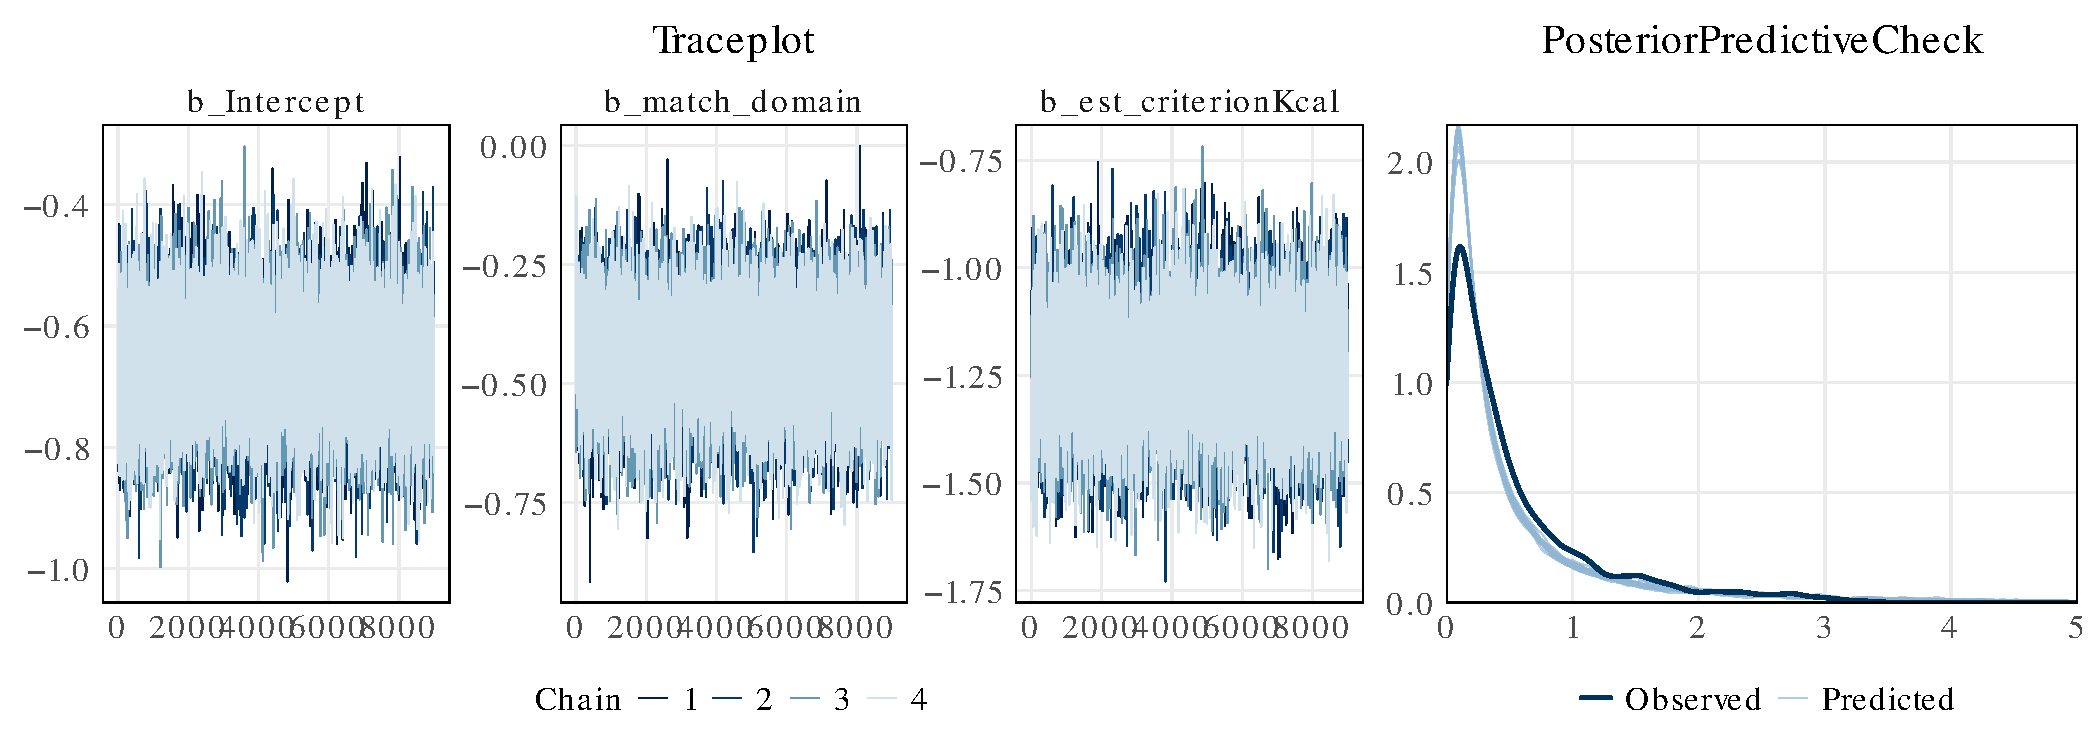
\includegraphics{supplement_files/figure-pdf/h3aM1-1.pdf}

\subsubsection{M2}\label{m2}

\begin{Shaded}
\begin{Highlighting}[]
\CommentTok{\# Load model }
\NormalTok{temp }\OtherTok{\textless{}{-}} \FunctionTok{brm}\NormalTok{(}\AttributeTok{file=}\StringTok{"../Results/fit\_H3a\_M2.rds"}\NormalTok{)}

\CommentTok{\# Print Formular}
\NormalTok{temp}\SpecialCharTok{$}\NormalTok{formula}
\end{Highlighting}
\end{Shaded}

\begin{verbatim}
OME_corr ~ match_domain * est_criterion + (1 | ID) + (est_criterion * match_domain | ID_item) 
\end{verbatim}

\begin{Shaded}
\begin{Highlighting}[]
\CommentTok{\# Make model parameter table}
\FunctionTok{model\_parameters}\NormalTok{(temp, }\AttributeTok{centrality =} \StringTok{"mean"}\NormalTok{, }\AttributeTok{dispersion =} \ConstantTok{TRUE}\NormalTok{, }
                 \AttributeTok{ci\_method =} \StringTok{"hdi"}\NormalTok{, }\AttributeTok{effects =} \StringTok{"all"}\NormalTok{) }\SpecialCharTok{\%\textgreater{}\%} 
  \FunctionTok{kable}\NormalTok{(}\AttributeTok{digits=}\DecValTok{2}\NormalTok{) }\SpecialCharTok{\%\textgreater{}\%} \FunctionTok{kable\_paper}\NormalTok{()}
\end{Highlighting}
\end{Shaded}

\begin{longtable*}[t]{lllrrrrrrrrl}
\toprule
Parameter & Effects & Component & Mean & SD & CI & CI\_low & CI\_high & pd & Rhat & ESS & Group\\
\midrule
b\_Intercept & fixed & conditional & -0.68 & 0.08 & 0.95 & -0.84 & -0.52 & 1.00 & 1 & 6688.79 & \\
b\_match\_domain & fixed & conditional & -0.67 & 0.15 & 0.95 & -0.96 & -0.39 & 1.00 & 1 & 5273.65 & \\
b\_est\_criterionKcal & fixed & conditional & -1.22 & 0.12 & 0.95 & -1.45 & -0.99 & 1.00 & 1 & 6273.80 & \\
b\_match\_domain:est\_criterionKcal & fixed & conditional & 0.44 & 0.19 & 0.95 & 0.08 & 0.80 & 0.99 & 1 & 6324.02 & \\
sd\_ID\_\_Intercept & random & conditional & 0.58 & 0.04 & 0.95 & 0.51 & 0.66 & 1.00 & 1 & 8283.63 & ID\\
\addlinespace
sd\_ID\_item\_\_Intercept & random & conditional & 0.30 & 0.03 & 0.95 & 0.24 & 0.37 & 1.00 & 1 & 15180.45 & ID\_item\\
sd\_ID\_item\_\_est\_criterionKcal & random & conditional & 0.44 & 0.05 & 0.95 & 0.35 & 0.54 & 1.00 & 1 & 10422.51 & ID\_item\\
sd\_ID\_item\_\_match\_domain & random & conditional & 0.16 & 0.03 & 0.95 & 0.09 & 0.22 & 1.00 & 1 & 32353.62 & ID\_item\\
sd\_ID\_item\_\_est\_criterionKcal:match\_domain & random & conditional & 0.17 & 0.05 & 0.95 & 0.08 & 0.26 & 1.00 & 1 & 26870.47 & ID\_item\\
cor\_ID\_item\_\_Intercept\_\_est\_criterionKcal & random & conditional & -0.53 & 0.11 & 0.95 & -0.73 & -0.32 & 1.00 & 1 & 9554.61 & ID\_item\\
\addlinespace
cor\_ID\_item\_\_Intercept\_\_match\_domain & random & conditional & 0.70 & 0.16 & 0.95 & 0.38 & 0.96 & 1.00 & 1 & 31296.82 & ID\_item\\
cor\_ID\_item\_\_est\_criterionKcal\_\_match\_domain & random & conditional & -0.44 & 0.21 & 0.95 & -0.84 & -0.04 & 0.97 & 1 & 34013.37 & ID\_item\\
cor\_ID\_item\_\_Intercept\_\_est\_criterionKcal:match\_domain & random & conditional & -0.50 & 0.24 & 0.95 & -0.90 & -0.02 & 0.97 & 1 & 35159.03 & ID\_item\\
cor\_ID\_item\_\_est\_criterionKcal\_\_est\_criterionKcal:match\_domain & random & conditional & 0.33 & 0.27 & 0.95 & -0.20 & 0.81 & 0.88 & 1 & 39931.20 & ID\_item\\
cor\_ID\_item\_\_match\_domain\_\_est\_criterionKcal:match\_domain & random & conditional & -0.59 & 0.24 & 0.95 & -0.96 & -0.11 & 0.98 & 1 & 24241.81 & ID\_item\\
\addlinespace
sigma & fixed & sigma & 1.05 & 0.01 & 0.95 & 1.03 & 1.07 & 1.00 & 1 & 83728.01 & \\
\bottomrule
\end{longtable*}

\begin{Shaded}
\begin{Highlighting}[]
\CommentTok{\# Make trace and pp{-}check plot}
\FunctionTok{brms\_plot}\NormalTok{(temp) }\SpecialCharTok{+} \FunctionTok{plot\_layout}\NormalTok{(}\AttributeTok{widths =} \FunctionTok{c}\NormalTok{(}\DecValTok{2}\NormalTok{, }\DecValTok{1}\NormalTok{))}
\end{Highlighting}
\end{Shaded}

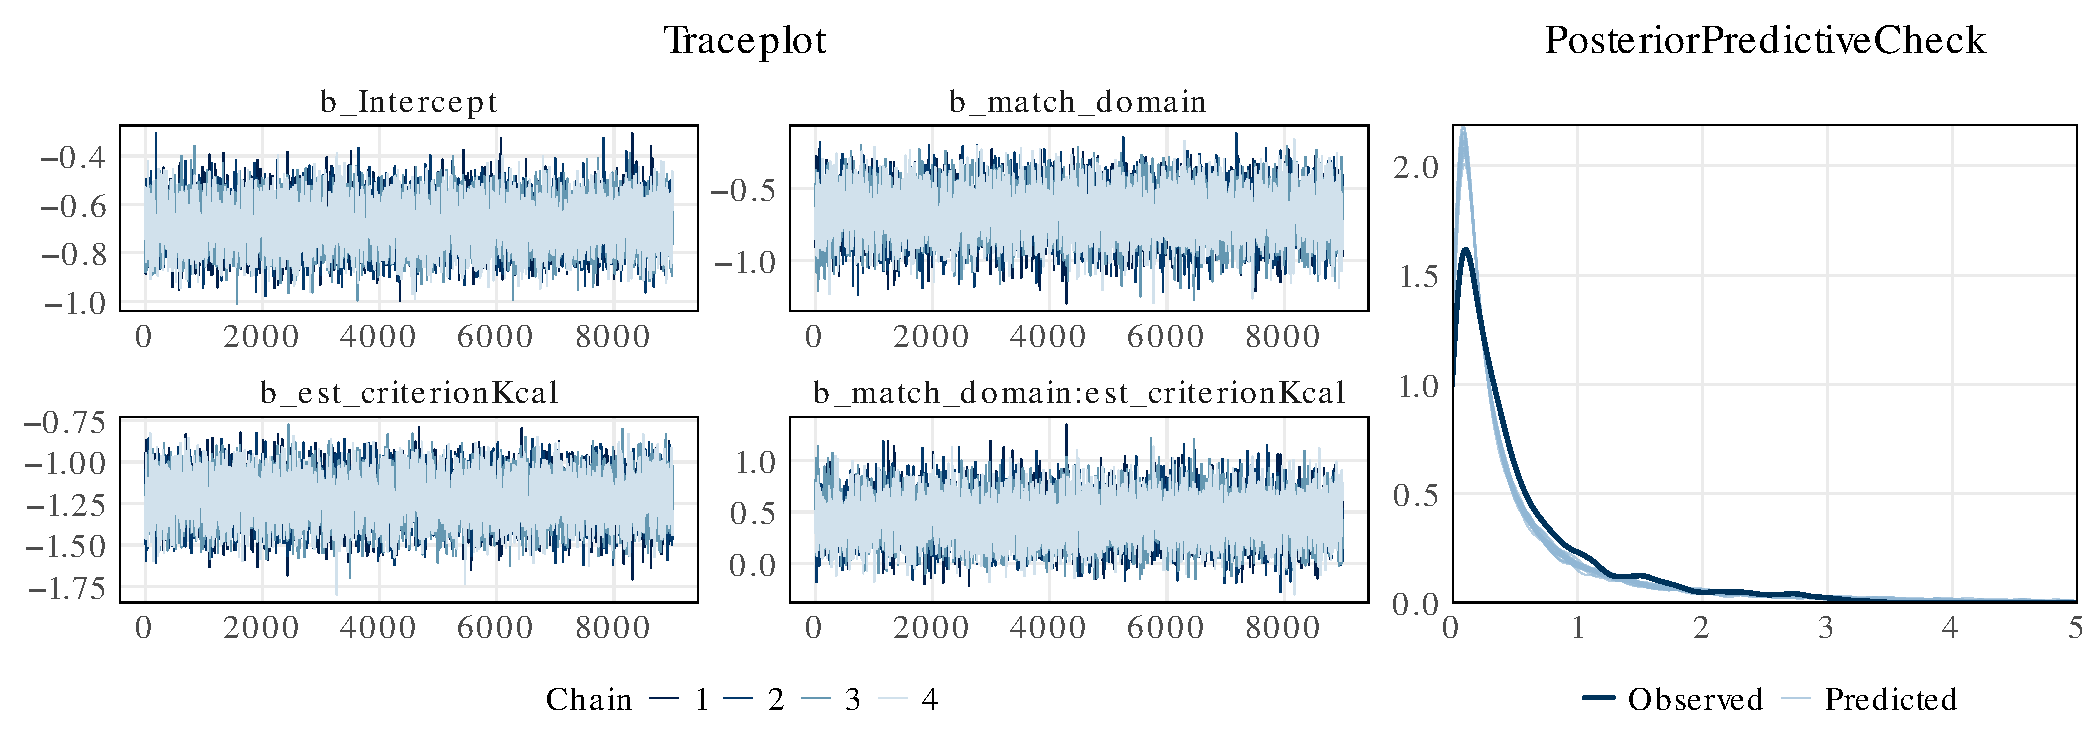
\includegraphics{supplement_files/figure-pdf/h3aM2-1.pdf}

\subsection{\texorpdfstring{Hypothesis 3b
(\(\rho\))}{Hypothesis 3b (\textbackslash rho)}}\label{hypothesis-3b-rho}

\subsubsection{M0}\label{m0-1}

\begin{Shaded}
\begin{Highlighting}[]
\CommentTok{\# Load model }
\NormalTok{temp }\OtherTok{\textless{}{-}} \FunctionTok{brm}\NormalTok{(}\AttributeTok{file=}\StringTok{"../Results/fit\_H3b\_M0.rds"}\NormalTok{)}

\CommentTok{\# Print Formular}
\NormalTok{temp}\SpecialCharTok{$}\NormalTok{formula}
\end{Highlighting}
\end{Shaded}

\begin{verbatim}
rank_z ~ match_domain + (1 | ID) 
\end{verbatim}

\begin{Shaded}
\begin{Highlighting}[]
\CommentTok{\# Make model parameter table}
\FunctionTok{model\_parameters}\NormalTok{(temp, }\AttributeTok{centrality =} \StringTok{"mean"}\NormalTok{, }\AttributeTok{dispersion =} \ConstantTok{TRUE}\NormalTok{, }
                 \AttributeTok{ci\_method =} \StringTok{"hdi"}\NormalTok{, }\AttributeTok{effects =} \StringTok{"all"}\NormalTok{) }\SpecialCharTok{\%\textgreater{}\%} 
  \FunctionTok{kable}\NormalTok{(}\AttributeTok{digits=}\DecValTok{2}\NormalTok{) }\SpecialCharTok{\%\textgreater{}\%} \FunctionTok{kable\_paper}\NormalTok{()}
\end{Highlighting}
\end{Shaded}

\begin{longtable*}[t]{lllrrrrrrrrl}
\toprule
Parameter & Effects & Component & Mean & SD & CI & CI\_low & CI\_high & pd & Rhat & ESS & Group\\
\midrule
b\_Intercept & fixed & conditional & 0.81 & 0.03 & 0.95 & 0.76 & 0.87 & 1.00 & 1.00 & 10661.50 & \\
b\_match\_domain & fixed & conditional & 0.07 & 0.05 & 0.95 & -0.03 & 0.18 & 0.92 & 1.00 & 12139.03 & \\
sd\_ID\_\_Intercept & random & conditional & 0.22 & 0.06 & 0.95 & 0.11 & 0.32 & 1.00 & 1.00 & 565.52 & ID\\
sigma & fixed & sigma & 0.23 & 0.06 & 0.95 & 0.10 & 0.32 & 1.00 & 1.01 & 342.18 & \\
\bottomrule
\end{longtable*}

\begin{Shaded}
\begin{Highlighting}[]
\CommentTok{\# Make trace and pp{-}check plot}
\FunctionTok{brms\_plot}\NormalTok{(temp) }\SpecialCharTok{+} \FunctionTok{plot\_layout}\NormalTok{(}\AttributeTok{widths =} \FunctionTok{c}\NormalTok{(}\DecValTok{2}\NormalTok{, }\DecValTok{1}\NormalTok{))}
\end{Highlighting}
\end{Shaded}

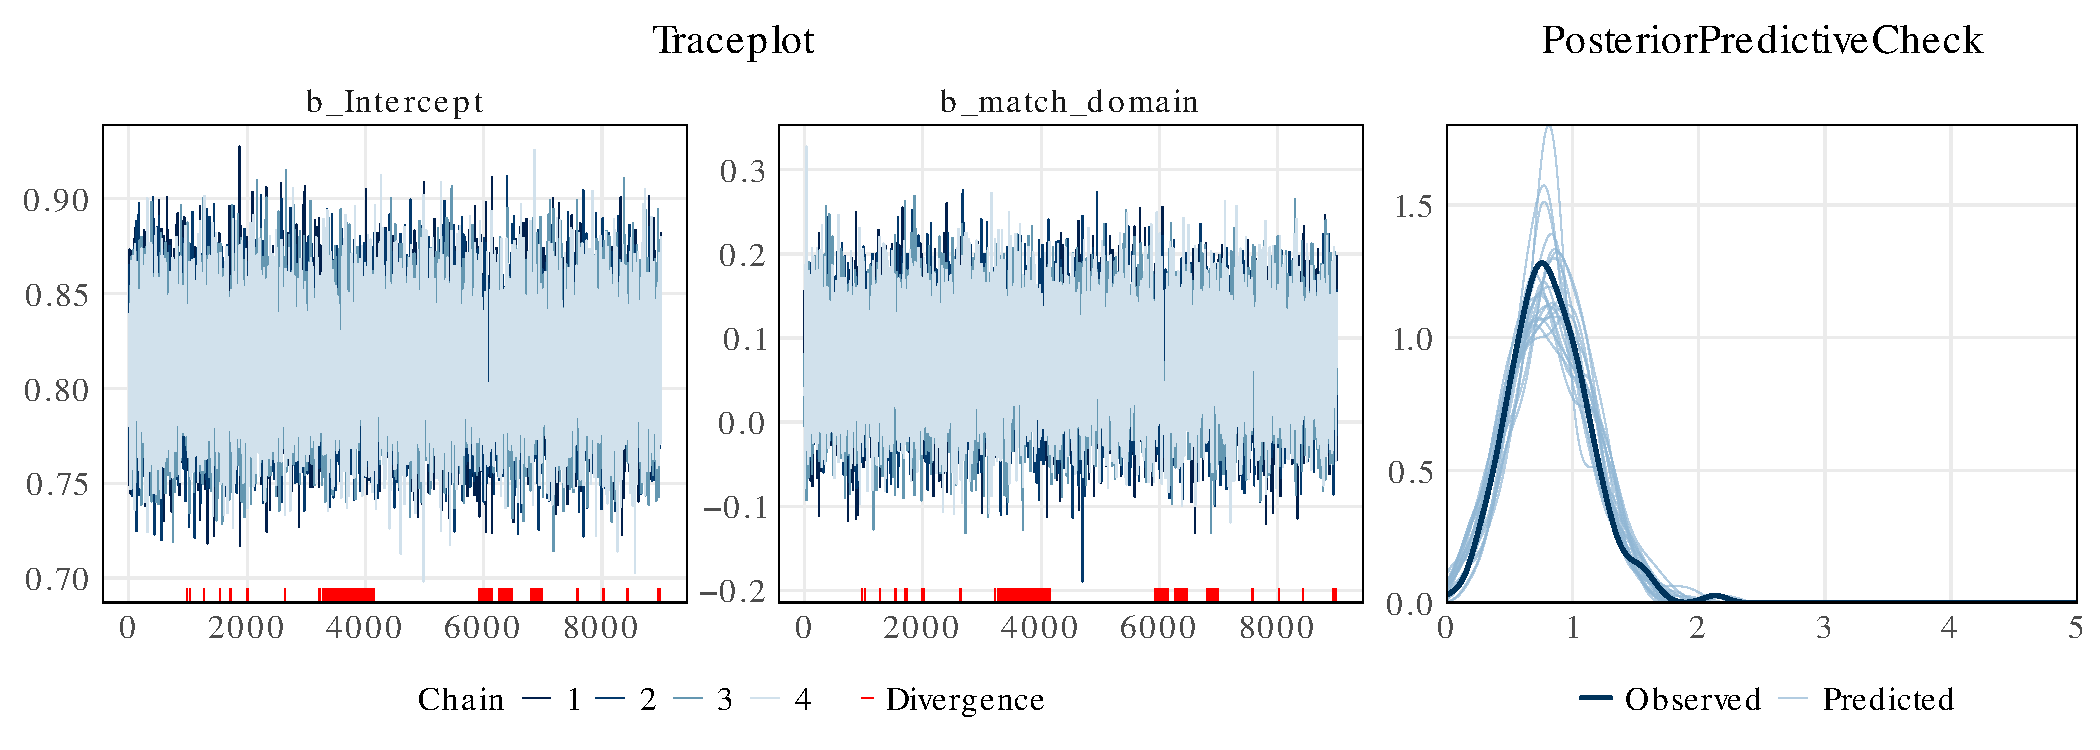
\includegraphics{supplement_files/figure-pdf/h3bM0-1.pdf}

\subsubsection{M1}\label{m1-1}

\begin{Shaded}
\begin{Highlighting}[]
\CommentTok{\# Load model }
\NormalTok{temp }\OtherTok{\textless{}{-}} \FunctionTok{brm}\NormalTok{(}\AttributeTok{file=}\StringTok{"../Results/fit\_H3b\_M1.rds"}\NormalTok{)}

\CommentTok{\# Print Formular}
\NormalTok{temp}\SpecialCharTok{$}\NormalTok{formula}
\end{Highlighting}
\end{Shaded}

\begin{verbatim}
rank_z ~ match_domain + est_criterion + (1 | ID) 
\end{verbatim}

\begin{Shaded}
\begin{Highlighting}[]
\CommentTok{\# Make model parameter table}
\FunctionTok{model\_parameters}\NormalTok{(temp, }\AttributeTok{centrality =} \StringTok{"mean"}\NormalTok{, }\AttributeTok{dispersion =} \ConstantTok{TRUE}\NormalTok{, }
                 \AttributeTok{ci\_method =} \StringTok{"hdi"}\NormalTok{, }\AttributeTok{effects =} \StringTok{"all"}\NormalTok{) }\SpecialCharTok{\%\textgreater{}\%} 
  \FunctionTok{kable}\NormalTok{(}\AttributeTok{digits=}\DecValTok{2}\NormalTok{) }\SpecialCharTok{\%\textgreater{}\%} \FunctionTok{kable\_paper}\NormalTok{()}
\end{Highlighting}
\end{Shaded}

\begin{longtable*}[t]{lllrrrrrrrrl}
\toprule
Parameter & Effects & Component & Mean & SD & CI & CI\_low & CI\_high & pd & Rhat & ESS & Group\\
\midrule
b\_Intercept & fixed & conditional & 0.71 & 0.04 & 0.95 & 0.64 & 0.78 & 1.00 & 1.00 & 17064.69 & \\
b\_match\_domain & fixed & conditional & 0.06 & 0.05 & 0.95 & -0.04 & 0.16 & 0.87 & 1.00 & 14577.88 & \\
b\_est\_criterionKcal & fixed & conditional & 0.20 & 0.05 & 0.95 & 0.10 & 0.31 & 1.00 & 1.00 & 15169.38 & \\
sd\_ID\_\_Intercept & random & conditional & 0.21 & 0.05 & 0.95 & 0.11 & 0.30 & 1.00 & 1.00 & 1029.88 & ID\\
sigma & fixed & sigma & 0.22 & 0.05 & 0.95 & 0.12 & 0.31 & 1.00 & 1.01 & 862.52 & \\
\bottomrule
\end{longtable*}

\begin{Shaded}
\begin{Highlighting}[]
\CommentTok{\# Make trace and pp{-}check plot}
\FunctionTok{brms\_plot}\NormalTok{(temp) }\SpecialCharTok{+} \FunctionTok{plot\_layout}\NormalTok{(}\AttributeTok{widths =} \FunctionTok{c}\NormalTok{(}\DecValTok{2}\NormalTok{, }\DecValTok{1}\NormalTok{))}
\end{Highlighting}
\end{Shaded}

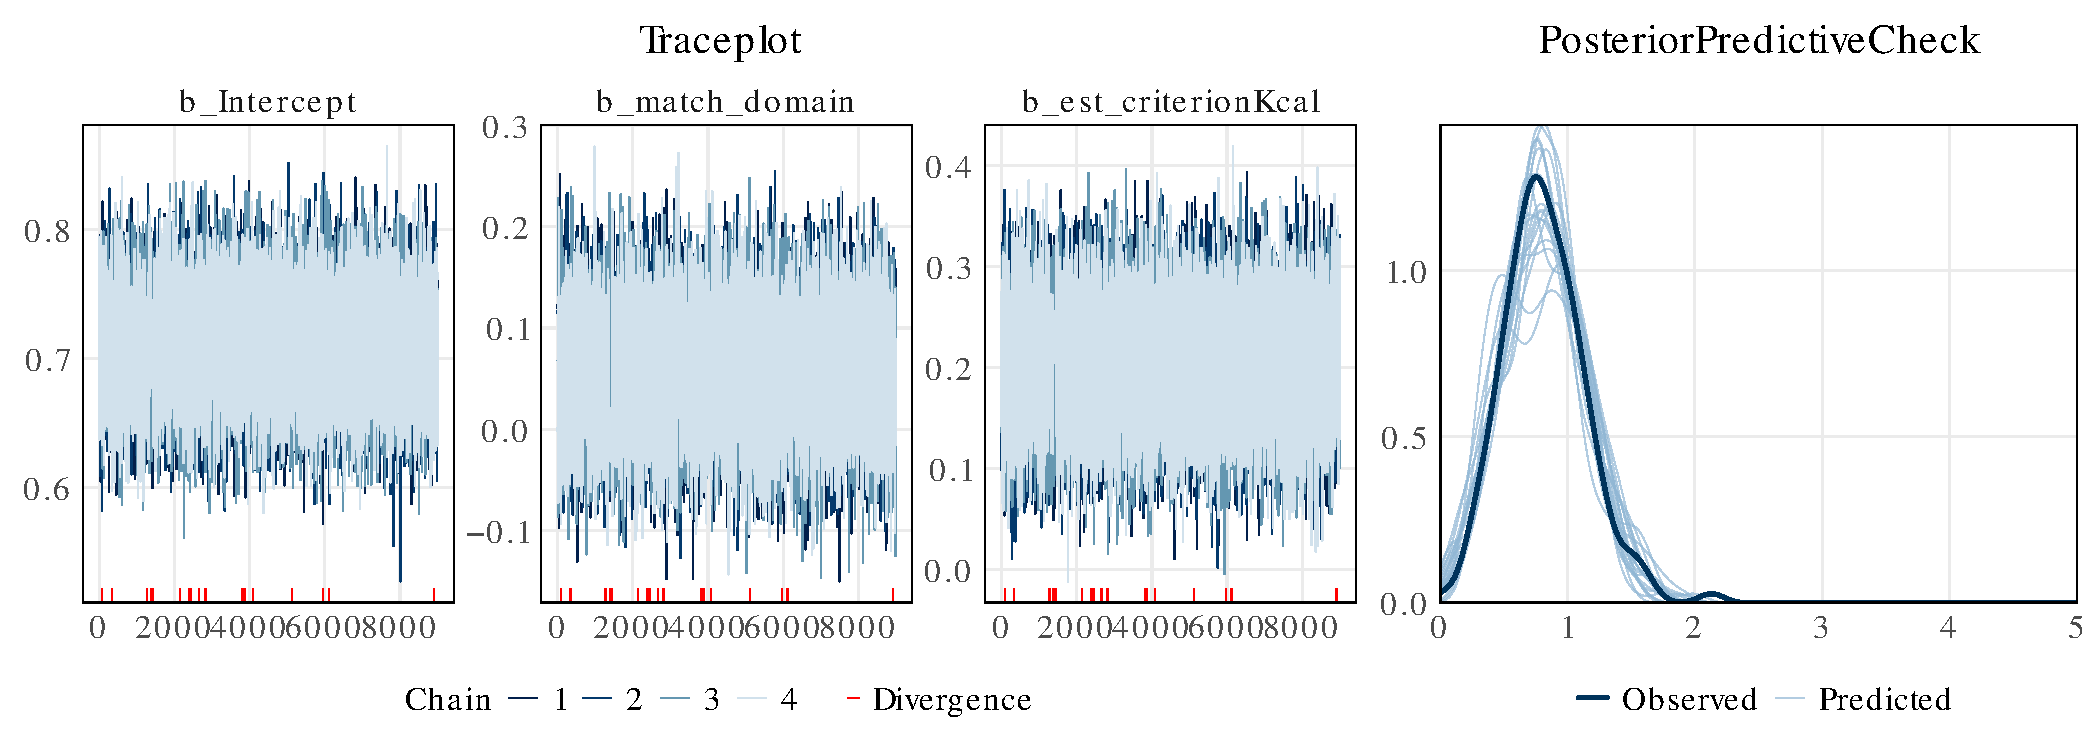
\includegraphics{supplement_files/figure-pdf/h3bM1-1.pdf}

\subsubsection{M2}\label{m2-1}

\begin{Shaded}
\begin{Highlighting}[]
\CommentTok{\# Load model }
\NormalTok{temp }\OtherTok{\textless{}{-}} \FunctionTok{brm}\NormalTok{(}\AttributeTok{file=}\StringTok{"../Results/fit\_H3b\_M2.rds"}\NormalTok{)}

\CommentTok{\# Print Formular}
\NormalTok{temp}\SpecialCharTok{$}\NormalTok{formula}
\end{Highlighting}
\end{Shaded}

\begin{verbatim}
rank_z ~ match_domain * est_criterion + (1 | ID) 
\end{verbatim}

\begin{Shaded}
\begin{Highlighting}[]
\CommentTok{\# Make model parameter table}
\FunctionTok{model\_parameters}\NormalTok{(temp, }\AttributeTok{centrality =} \StringTok{"mean"}\NormalTok{, }\AttributeTok{dispersion =} \ConstantTok{TRUE}\NormalTok{, }
                 \AttributeTok{ci\_method =} \StringTok{"hdi"}\NormalTok{, }\AttributeTok{effects =} \StringTok{"all"}\NormalTok{) }\SpecialCharTok{\%\textgreater{}\%} 
  \FunctionTok{kable}\NormalTok{(}\AttributeTok{digits=}\DecValTok{2}\NormalTok{) }\SpecialCharTok{\%\textgreater{}\%} \FunctionTok{kable\_paper}\NormalTok{()}
\end{Highlighting}
\end{Shaded}

\begin{longtable*}[t]{lllrrrrrrrrl}
\toprule
Parameter & Effects & Component & Mean & SD & CI & CI\_low & CI\_high & pd & Rhat & ESS & Group\\
\midrule
b\_Intercept & fixed & conditional & 0.71 & 0.04 & 0.95 & 0.63 & 0.78 & 1.00 & 1.00 & 14080.65 & \\
b\_match\_domain & fixed & conditional & 0.01 & 0.07 & 0.95 & -0.13 & 0.15 & 0.55 & 1.00 & 11724.21 & \\
b\_est\_criterionKcal & fixed & conditional & 0.21 & 0.05 & 0.95 & 0.10 & 0.31 & 1.00 & 1.00 & 15907.01 & \\
b\_match\_domain:est\_criterionKcal & fixed & conditional & 0.10 & 0.10 & 0.95 & -0.10 & 0.30 & 0.83 & 1.00 & 8126.98 & \\
sd\_ID\_\_Intercept & random & conditional & 0.21 & 0.06 & 0.95 & 0.11 & 0.31 & 1.00 & 1.01 & 865.65 & ID\\
\addlinespace
sigma & fixed & sigma & 0.22 & 0.06 & 0.95 & 0.10 & 0.31 & 1.00 & 1.01 & 661.23 & \\
\bottomrule
\end{longtable*}

\begin{Shaded}
\begin{Highlighting}[]
\CommentTok{\# Make trace and pp{-}check plot}
\FunctionTok{brms\_plot}\NormalTok{(temp) }\SpecialCharTok{+} \FunctionTok{plot\_layout}\NormalTok{(}\AttributeTok{widths =} \FunctionTok{c}\NormalTok{(}\DecValTok{2}\NormalTok{, }\DecValTok{1}\NormalTok{))}
\end{Highlighting}
\end{Shaded}

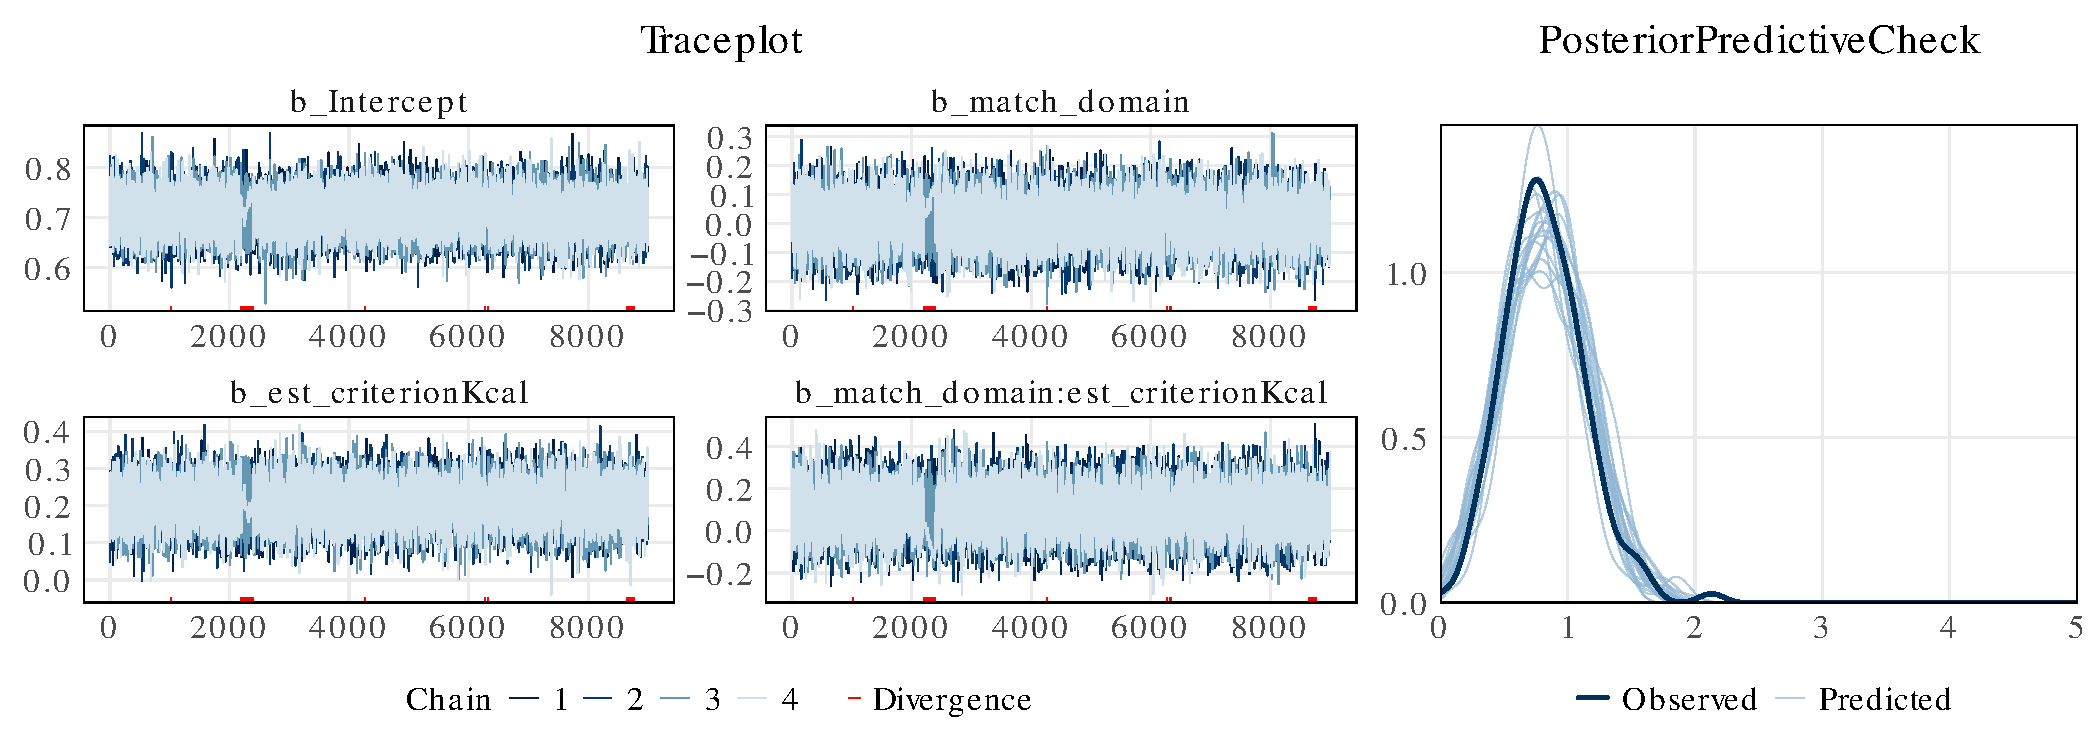
\includegraphics{supplement_files/figure-pdf/h3bM2-1.pdf}



\end{document}
